%-----------------------------------
% Define document and include general packages
%-----------------------------------
% Tabellen- und Abbildungsverzeichnis stehen normalerweise nicht im
% Inhaltsverzeichnis. Gleiches gilt für das Abkürzungsverzeichnis (siehe unten).
% Manche Dozenten bemängeln das. Die Optionen 'listof=totoc,bibliography=totoc'
% geben das Tabellen- und Abbildungsverzeichnis im Inhaltsverzeichnis (toc=Table
% of Content) aus.
% Da es aber verschiedene Regelungen je nach Dozent geben kann, werden hier
% beide Varianten dargestellt.
\documentclass[12pt,oneside,titlepage,listof=totoc,bibliography=totoc]{scrartcl}
%\documentclass[12pt,oneside,titlepage]{scrartcl}

%-----------------------------------
% Dokumentensprache
%-----------------------------------
\def\FOMEN{}% Auskommentieren um die Dokumentensprache auf englisch zu ändern
\newif\ifde
\newif\ifen

%-----------------------------------
% Meta informationen
%-----------------------------------
%-----------------------------------
% Meta Informationen zur Arbeit
%-----------------------------------

% Autor
\newcommand{\myAutor}{Thomas Keiser\\Martin Krüger\\Jesper Wesemann\\Luis Pflamminger}

% Titel der Arbeit
\newcommand{\myTitel}{Predicting Music Genres based on Spotify Song Data using a Gradient Boosting Algorithm}

% Betreuer
\newcommand{\myBetreuer}{Prof. Dr. Adem Alparslan}

% Lehrveranstaltung
\newcommand{\myLehrveranstaltung}{Big Data \& Data Science}

% Matrikelnummer
\newcommand{\myMatrikelNr}{123456 (Krüger), 123456 (Keiser),123456 (Wesemann), 123456 (Pflamminger)}

% Ort
\newcommand{\myOrt}{Düsseldorf}

% Datum der Abgabe
\newcommand{\myAbgabeDatum}{January 31st, 2022}

% Semesterzahl
\newcommand{\mySemesterZahl}{5}

% Name der Hochschule
\newcommand{\myHochschulName}{FOM Hochschule für Oekonomie \& Management}

% Standort der Hochschule
\newcommand{\myHochschulStandort}{Düsseldorf}

% Studiengang
\newcommand{\myStudiengang}{"Wirtschaftsinformatik"}

% Art der Arbeit
\newcommand{\myThesisArt}{Scientific Paper}

% Zu erlangender akademische Grad
\newcommand{\myAkademischerGrad}{Bachelor of Science (B.Sc.)}

% Firma
\newcommand{\myFirma}{Deutsche Telekom AG}


\ifdefined\FOMEN
%Englisch
\entrue
\usepackage[english]{babel}
\else
%Deutsch
\detrue
\usepackage[ngerman]{babel}
\fi


\newcommand{\langde}[1]{%
   \ifde\selectlanguage{ngerman}#1\fi}
\newcommand{\langen}[1]{%
   \ifen\selectlanguage{english}#1\fi}
\usepackage[utf8]{luainputenc}
\langde{\usepackage[babel,german=quotes]{csquotes}}
\langen{\usepackage[babel,english=british]{csquotes}}
\usepackage[T1]{fontenc}
\usepackage{fancyhdr}
\usepackage{fancybox}
\usepackage[a4paper, left=4cm, right=2cm, top=4cm, bottom=2cm]{geometry}
\usepackage{graphicx}
\usepackage{subfig}
\usepackage{wrapfig}
\usepackage{colortbl}
\usepackage[capposition=top]{floatrow}
\usepackage{array}
\usepackage{float}      %Positionierung von Abb. und Tabellen mit [H] erzwingen
\usepackage{footnote}
% Darstellung der Beschriftung von Tabellen und Abbildungen (Leitfaden S. 44)
% singlelinecheck=false: macht die Caption linksbündig (statt zentriert)
% labelfont auf fett: (Tabelle x.y:, Abbildung: x.y)
% font auf fett: eigentliche Bezeichnung der Abbildung oder Tabelle
% Fettschrift laut Leitfaden 2018 S. 45
\usepackage[singlelinecheck=false, labelfont=bf, font=bf]{caption}
\usepackage{caption}
\usepackage{enumitem}
\usepackage{amssymb}
\usepackage{mathptmx}
%\usepackage{minted} %Kann für schöneres Syntax Highlighting genutzt werden. ACHTUNG: Python muss installiert sein.
\usepackage[scaled=0.9]{helvet} % Behebt, zusammen mit Package courier, pixelige Überschriften. Ist, zusammen mit mathptx, dem times-Package vorzuziehen. Details: https://latex-kurs.de/fragen/schriftarten/Times_New_Roman.html
\usepackage{courier}
\usepackage{amsmath}
\usepackage[table]{xcolor}
\usepackage{marvosym}			% Verwendung von Symbolen, z.B. perfektes Eurozeichen

\renewcommand\familydefault{\sfdefault}
\usepackage{ragged2e}

% Mehrere Fussnoten nacheinander mit Komma separiert
\usepackage[hang,multiple]{footmisc}
\setlength{\footnotemargin}{1em}

% todo Aufgaben als Kommentare verfassen für verschiedene Editoren
\usepackage{todonotes}

% Verhindert, dass nur eine Zeile auf der nächsten Seite steht
\setlength{\marginparwidth}{2cm}
\usepackage[all]{nowidow}

%-----------------------------------
% Farbdefinitionen
%-----------------------------------
\definecolor{darkblack}{rgb}{0,0,0}
\definecolor{dunkelgrau}{rgb}{0.8,0.8,0.8}
\definecolor{hellgrau}{rgb}{0.0,0.7,0.99}
\definecolor{mauve}{rgb}{0.58,0,0.82}
\definecolor{dkgreen}{rgb}{0,0.6,0}

%-----------------------------------
% Pakete für Tabellen
%-----------------------------------
\usepackage{epstopdf}
\usepackage{nicefrac} % Brüche
\usepackage{multirow}
\usepackage{rotating} % vertikal schreiben
\usepackage{mdwlist}
\usepackage{tabularx}% für Breitenangabe

%-----------------------------------
% sauber formatierter Quelltext
%-----------------------------------
\usepackage{listings}
% JavaScript als Sprache definieren:
\lstdefinelanguage{JavaScript}{
	keywords={break, super, case, extends, switch, catch, finally, for, const, function, try, continue, if, typeof, debugger, var, default, in, void, delete, instanceof, while, do, new, with, else, return, yield, enum, let, await},
	keywordstyle=\color{blue}\bfseries,
	ndkeywords={class, export, boolean, throw, implements, import, this, interface, package, private, protected, public, static},
	ndkeywordstyle=\color{darkgray}\bfseries,
	identifierstyle=\color{black},
	sensitive=false,
	comment=[l]{//},
	morecomment=[s]{/*}{*/},
	commentstyle=\color{purple}\ttfamily,
	stringstyle=\color{red}\ttfamily,
	morestring=[b]',
	morestring=[b]"
}

\lstset{
	%language=JavaScript,
	numbers=left,
	numberstyle=\tiny,
	numbersep=5pt,
	breaklines=true,
	showstringspaces=false,
	frame=single ,
	xleftmargin=5pt,
	xrightmargin=5pt,
	basicstyle=\ttfamily\scriptsize,
	stepnumber=1,
	keywordstyle=\color{blue},          % keyword style
  	commentstyle=\color{dkgreen},       % comment style
  	stringstyle=\color{mauve}         % string literal style
}

%-----------------------------------
%Literaturverzeichnis Einstellungen
%-----------------------------------

% Biblatex

\usepackage{url}
\urlstyle{same}

%%%% Neuer Leitfaden (2018)
\usepackage[
backend=biber,
style=ieee,
maxcitenames=3,	% mindestens 3 Namen ausgeben bevor et. al. kommt
maxbibnames=999,
date=iso,
seconds=true, %werden nicht verwendet, so werden aber Warnungen unterdrückt.
urldate=iso,
dashed=false,
autocite=inline,
useprefix=true, % 'von' im Namen beachten (beim Anzeigen)
mincrossrefs = 1
]{biblatex}%iso dateformat für YYYY-MM-DD

%weitere Anpassungen für BibLaTex
%\usepackage{xpatch}

\setlength\bibhang{1cm}

%%% Weitere Optionen
%\boolitem[false]{citexref} %Wenn incollection, inbook, inproceedings genutzt wird nicht den zugehörigen parent auch in Literaturverzeichnis aufnehmen

%Aufräumen die Felder werden laut Leitfaden nicht benötigt.
\AtEveryBibitem{%
\ifentrytype{book}{
    \clearfield{issn}%
    \clearfield{doi}%
    \clearfield{isbn}%
    \clearfield{url}
    \clearfield{eprint}
}{}
\ifentrytype{collection}{
  \clearfield{issn}%
  \clearfield{doi}%
  \clearfield{isbn}%
  \clearfield{url}
  \clearfield{eprint}
}{}
\ifentrytype{incollection}{
  \clearfield{issn}%
  \clearfield{doi}%
  \clearfield{isbn}%
  \clearfield{url}
  \clearfield{eprint}
}{}
\ifentrytype{article}{
  \clearfield{issn}%
  \clearfield{doi}%
  \clearfield{isbn}%
  \clearfield{url}
  \clearfield{eprint}
}{}
\ifentrytype{inproceedings}{
  \clearfield{issn}%
  \clearfield{doi}%
  \clearfield{isbn}%
  \clearfield{url}
  \clearfield{eprint}
}{}
}

\renewcommand*{\finentrypunct}{}%Kein Punkt am ende des Literaturverzeichnisses

\renewcommand*{\newunitpunct}{\addcomma\space}
\DeclareDelimFormat[bib,biblist]{nametitledelim}{\addcolon\space}
\DeclareDelimFormat{titleyeardelim}{\newunitpunct}
%Namen kursiv schreiben
\renewcommand*{\mkbibnamefamily}{\mkbibemph}
\renewcommand*{\mkbibnamegiven}{\mkbibemph}
\renewcommand*{\mkbibnamesuffix}{\mkbibemph}
\renewcommand*{\mkbibnameprefix}{\mkbibemph}

% Die Trennung mehrerer Autorennamen erfolgt durch Kommata.
% siehe Beispiele im Leitfaden S. 16
% Die folgende Zeile würde mit Semikolon trennen
%\DeclareDelimFormat{multinamedelim}{\addsemicolon\addspace}

%Delimiter für mehrere und letzten Namen gleich setzen
\DeclareDelimAlias{finalnamedelim}{multinamedelim}

\DeclareNameAlias{default}{family-given}
\DeclareNameAlias{sortname}{default}  %Nach Namen sortieren


\DeclareFieldFormat{editortype}{\mkbibparens{#1}}
\DeclareDelimFormat{editortypedelim}{\addspace}
\DeclareFieldFormat{translatortype}{\mkbibparens{#1}}
\DeclareDelimFormat{translatortypedelim}{\addspace}
\DeclareDelimFormat[bib,biblist]{innametitledelim}{\addcomma\space}

\DeclareFieldFormat*{citetitle}{#1}
\DeclareFieldFormat*{title}{#1}
\DeclareFieldFormat*{booktitle}{#1}
\DeclareFieldFormat*{journaltitle}{#1}

\xpatchbibdriver{online}
  {\usebibmacro{organization+location+date}\newunit\newblock}
  {}
  {}{}

\DeclareFieldFormat[online]{date}{\mkbibparens{#1}}
\DeclareFieldFormat{urltime}{\addspace #1\addspace \langde{Uhr}\langen{MEZ}}
\DeclareFieldFormat{urldate}{%urltime zu urldate hinzufügen
  [\langde{Zugriff}\langen{Access}\addcolon\addspace
  #1\printfield{urltime}]
}
\DeclareFieldFormat[online]{url}{<\url{#1}>}
\renewbibmacro*{url+urldate}{%
  \usebibmacro{url}%
  \ifentrytype{online}
    {\setunit*{\addspace}%
     \iffieldundef{year}
       {\printtext[date]{\langde{keine Datumsangabe}\langen{no Date} }}
       {\usebibmacro{date}}}%
    {}%
  \setunit*{\addspace}%
  \usebibmacro{urldate}
  }

%Verhindern, dass bei mehreren Quellen des gleichen Autors im gleichen Jahr
%Buchstaben nach der Jahreszahl angezeigt werden wenn sich das Keyword in usera unterscheidet.
\DeclareExtradate{
  \scope{
    \field{labelyear}
    \field{year}
    }
    \scope{
      \field{usera}
     }
}

%% Anzeige des Jahres nach dem Stichwort (usera) im Literaturverzeichnis
%% Wenn das Jahr bei Online-Quellen nicht explizit angegeben wurde, wird nach
%% dem Stichwort 'o. J.' ausgegeben. Nach der URL steht dann 'keine
%% Datumsangabe'. Ist das Jahr definiert, wird es an beiden Stellen ausgegeben.
%% Das Zugriffsdatum (urldate) spielt hier keine Rolle.
%% Für Nicht-Online-Quellen wird nichts geändert.
\renewbibmacro*{date+extradate}{%
  \printtext[parens]{%
    \printfield{usera}%
    \setunit{\printdelim{titleyeardelim}}%
    \ifentrytype{online}
       {\setunit*{\addspace\addcomma\addspace}%
         \iffieldundef{year}
           {\bibstring{nodate}}
       {\printlabeldateextra}}%
       {\printlabeldateextra}}}

%% Anzeige des Jahres nach dem Stichwort (usera) in der Fussnote
%% das Stichwort hat der Aufrufer hier schon ausgegeben.
%% siehe auch Kommentar zu: \renewbibmacro*{date+extradate}
\renewbibmacro*{cite:labeldate+extradate}{%
    \ifentrytype{online}
       {\setunit*{\addspace\addcomma\addspace}%
         \iffieldundef{year}
           {\bibstring{nodate}}
       {\printlabeldateextra}}%
       {\printlabeldateextra}}


\DefineBibliographyStrings{german}{
  nodate    = {{}o.\adddot\addspace J\adddot},
  andothers = {et\addabbrvspace al\adddot}
}
\DefineBibliographyStrings{english}{
  nodate    = {{}n.\adddot\addspace d\adddot},
  andothers = {et\addabbrvspace al\adddot}
}
\DeclareSourcemap{
  \maps[datatype=bibtex]{
    \map{
      \step[notfield=translator, final]
      \step[notfield=editor, final]
      \step[fieldset=author, fieldvalue={{{\langde{o\noexpand\adddot\addspace V\noexpand\adddot}\langen{Anon}}}}]
    }
    \map{
      \pernottype{online}
      \step[fieldset=location, fieldvalue={\langde{o\noexpand\adddot\addspace O\noexpand\adddot}\langen{s\noexpand\adddot I\noexpand\adddot}}]
    }
  }
}

\renewbibmacro*{cite}{%
  \iffieldundef{shorthand}
    {\ifthenelse{\ifnameundef{labelname}\OR\iffieldundef{labelyear}}
       {\usebibmacro{cite:label}%
        \setunit{\printdelim{nonametitledelim}}}
       {\printnames{labelname}%
        \setunit{\printdelim{nametitledelim}}}%
     \printfield{usera}%
     \setunit{\printdelim{titleyeardelim}}%
     \usebibmacro{cite:labeldate+extradate}}
    {\usebibmacro{cite:shorthand}}}

    \renewcommand*{\jourvoldelim}{\addcomma\addspace}% Trennung zwischen journalname und Volume. Sonst Space; Laut Leitfaden richtig
    %Aufgrund der Änderung bzgl des Issues 169 in der thesis_main.tex musste ich die Zeile auskommentieren. Konnte aber das Verhalten, dass die Fußnoten grün sind, im nachhinein nicht feststellen.
    %\hypersetup{hidelinks} %sonst sind Fußnoten grün. Dadurch werden Links allerdings nicht mehr farbig dargestellt

\renewbibmacro*{journal+issuetitle}{%
  \usebibmacro{journal}%
  \setunit*{\jourvoldelim}%
  \iffieldundef{series}
    {}
    {\setunit*{\jourserdelim}%
     \printfield{series}%
     \setunit{\servoldelim}}%
  \iffieldundef{volume}
    {}
    {\printfield{volume}}
  \iffieldundef{labelyear}
  {}
  {
  (\thefield{year}) %Ansonsten wird wenn kein Volume angegeben ist ein Komma vorangestellt
  }
  \setunit*{\addcomma\addspace Nr\adddot\addspace}
  \printfield{number}
  \iffieldundef{eid}
  {}
  {\printfield{eid}}
}

% Postnote ist der Text in der zweiten eckigen Klammer bei einem Zitat
% wenn es keinen solchen Eintrag gibt, dann auch nicht ausgeben, z.B. 'o. S.'
% Wenn man das will, kann man das 'o. S.' ja explizit angeben. Andernfalls steht
% sonst auch bei Webseiten 'o. S.' da, was laut Leitfaden nicht ok ist.
\renewbibmacro*{postnote}{%
  \setunit{\postnotedelim}%
  \iffieldundef{postnote}
    {} %{\printtext{\langde{o.S\adddot}\langen{no page number}}}
    {\printfield{postnote}}}

% Abstand bei Änderung Anfangsbuchstabe ca. 1.5 Zeilen
\setlength{\bibinitsep}{0.75cm}

% nur in den Zitaten/Fussnoten den Vornamen abkürzen (nicht im
% Literaturverzeichnis)

\DeclareDelimFormat{nonameyeardelim}{\addcomma\space}
\DeclareDelimFormat{nameyeardelim}{\addcomma\space}

\renewbibmacro*{cite}{%
  \iffieldundef{shorthand}
    {\ifthenelse{\ifciteibid\AND\NOT\iffirstonpage}
       {\usebibmacro{cite:ibid}}
    {\printtext[bibhyperref]{\ifthenelse{\ifnameundef{labelname}\OR\iffieldundef{labelyear}}
       {\usebibmacro{cite:label}%
        \setunit{\printdelim{nonameyeardelim}}}
      {\toggletrue{abx@bool@giveninits}%
        \printnames[family-given]{labelname}%
        \setunit{\printdelim{nameyeardelim}}}%
      \printfield{usera}%
      \setunit{\printdelim{titleyeardelim}}%
     \usebibmacro{cite:labeldate+extradate}}}}
   {\usebibmacro{cite:shorthand}}}

%% et al. anstatt u. a. bei mehr als drei Autoren.
\DefineBibliographyStrings{ngerman}{ 
	andothers = {{et\,al\adddot}},             
}
\DefineBibliographyStrings{english}{ 
	andothers = {{et\,al\adddot}},             
}


%%%%% Alter Leitfaden. Ggf. Einkommentieren und Bereich hierüber auskommentieren
%\usepackage[
%backend=biber,
%style=numeric,
%citestyle=authoryear,
%url=false,
%isbn=false,
%notetype=footonly,
%hyperref=false,
%sortlocale=de]{biblatex}

%weitere Anpassungen für BibLaTex
%% Opptionen für Biblatex
\ExecuteBibliographyOptions{%
giveninits=false,
isbn=true,
url=true,
doi=false,
eprint=false,
maxbibnames=7, % Alle Autoren (kein et al.)
maxcitenames=2, % et al. ab dem 3. Autor
backref=false, % Rückverweise auf Zitatseiten
bibencoding=utf8, % wenn .bib in utf8, sonst ascii
bibwarn=true, % Warnung bei fehlerhafter bib-Datei
}%

% et al. an Stelle von u.a.
\DefineBibliographyStrings{ngerman}{
   andothers = {{et\,al\adddot}},
}

% Klammern um das Jahr in der Fußnote
\renewbibmacro*{cite:labelyear+extrayear}{%
  \iffieldundef{labelyear}
    {}
    {\printtext[bibhyperref]{%
       \mkbibparens{%
         \printfield{labelyear}%
         \printfield{extrayear}}}}}

\renewbibmacro*{cite:title}{%
  \printtext[bibhyperref]{%
    \printfield[citetitle]{labeltitle}%
    \setunit{\addcomma\space}%
    \printdate}}

\DeclareNameFormat{last-first}{%
  \iffirstinits
    {\usebibmacro{name:family-given}
        {\namepartfamily}
        {\namepartgiveni}
        {\namepartprefix}
        {\namepartsuffix}
    }
    {\usebibmacro{name:family-given}
        {\namepartfamily}
        {\namepartgiven}
        {\namepartprefix}
        {\namepartsuffix}
    }%
  \usebibmacro{name:andothers}}

% Alternative Notation der Fußnoten
% Zeigt sowohl den Nachnamen als auch den Vornamen an
% Beispiel: \fullfootcite[Vgl. ][Seite 5]{Tanenbaum.2003}
\DeclareCiteCommand{\fullfootcite}[\mkbibfootnote]
  {\usebibmacro{prenote}}
  {\usebibmacro{citeindex}%
    \printnames[sortname][1-1]{author}%
    \addspace (\printfield{year})}
  {\addsemicolon\space}
  {\usebibmacro{postnote}}

%Autoren (Nachname, Vorname)
\DeclareNameAlias{default}{family-given}

%Reihenfolge von publisher, year, address verändern
% Achtung, bisher nur für den Typ @book definiert

%% Definiert @Book Eintrag
\DeclareBibliographyDriver{book}{%
  \printnames{author}%
  \newunit\addcolon\space
  \printfield{title}%
  \setunit*{,\space}%
  \printfield{edition}%
  \setunit*{\addcomma\space}%
  \printlist{publisher}%
  \newunit\newblockpunct
  \printlist{location}%
  \setunit*{\space}%
  \printfield{year}%
  \setunit*{,\space}%
  \printfield{isbn}%
  \finentry}

%% Definiert @Online Eintrag
\DeclareBibliographyDriver{online}{%
  \printnames{author}%
  \newunit\newblockpunct
  \printfield{title}%
  \setunit*{,\space}%
  %\newunit\newblock
  \printfield{url}%
  \setunit*{,\space Erscheinungsjahr:\space}%
  \printfield{year}%
  \setunit*{,\space Aufruf am:\space}%
  \printfield{note}%
  \finentry}

%% Definiert @Article Eintrag
\DeclareBibliographyDriver{article}{%
  \printnames{author}%
  \newunit\newblockpunct
  \printfield{title}%
  \setunit*{.\space In:\space}%
  %\newunit\newblock
  \usebibmacro{journal}%
  \setunit*{\space (}%
  \printfield{year}\newunit{)}%
  \finentry}

%% Definiert @InProceedings Eintrag
\DeclareBibliographyDriver{inproceedings}{%
	\printnames{author}%
	\setunit*{,\space (}%
	\printfield{year}\newunit{)}%
	\newunit\newblockpunct
	\printfield{title}%
	\setunit*{\space}%
	\usebibmacro{booktitle}%
	\setunit*{,\space}%
	\printfield{isbn}%
	\setunit*{,\space}%
	\printfield{doi}%
	\finentry}

%Doppelpunkt nach dem letzten Autor
\renewcommand*{\labelnamepunct}{\addcolon\addspace }

%Komma an Stelle des Punktes
\renewcommand*{\newunitpunct}{\addcomma\space}

%Autoren durch Semikolon trennen
\newcommand*{\bibmultinamedelim}{\addsemicolon\space}%
\newcommand*{\bibfinalnamedelim}{\addsemicolon\space}%
\AtBeginBibliography{%
  \let\multinamedelim\bibmultinamedelim
  \let\finalnamedelim\bibfinalnamedelim
}

%Titel nicht kursiv anzeigen
\DeclareFieldFormat{title}{#1\isdot}


%%%% Ende Alter Leitfaden

%Bib-Datei einbinden
\addbibresource{literature/literature.bib}

% Zeilenabstand im Literaturverzeichnis ist Einzeilig
% siehe Leitfaden S. 14
\AtBeginBibliography{\singlespacing}

%-----------------------------------
% Silbentrennung
%-----------------------------------
\usepackage{hyphsubst}
\HyphSubstIfExists{ngerman-x-latest}{%
\HyphSubstLet{ngerman}{ngerman-x-latest}}{}

%-----------------------------------
% Pfad fuer Abbildungen
%-----------------------------------
\graphicspath{{./}{./figures/}}

%-----------------------------------
% Weitere Ebene einfügen
%-----------------------------------
\usepackage{titletoc}

\makeatletter

% Setze die Tiefe des Inhaltsverzeichnis auf 4 Ebenen
% Damit erscheinen \paragraph-Sektionen auch im Inhaltsverzeichnis
\setcounter{secnumdepth}{4}
\setcounter{tocdepth}{4}

% Fuege Abstand nach unten wie in einer normalen \section hinzu
% Andernfalls haette \paragraph keinen Zeilenumbruch
% Der Zeilenumbruch koennte mit einer leeren \mbox{} ersetzt werden
% Jedoch klebt dann der Text relativ nah an der Ueberschrift
\renewcommand{\paragraph}{%
  \@startsection{paragraph}{4}%
  {\z@}{3.25ex \@plus 1ex \@minus .2ex}{1.5ex plus 0.2ex}%
  {\normalfont\normalsize\bfseries\sffamily}%
}

\makeatother


%-----------------------------------
% Paket für die Nutzung von Anhängen
%-----------------------------------
\usepackage{appendix}

%-----------------------------------
% Zeilenabstand 1,5-zeilig
%-----------------------------------
\usepackage{setspace}
\onehalfspacing

%-----------------------------------
% Absätze durch eine neue Zeile
%-----------------------------------
\setlength{\parindent}{0mm}
\setlength{\parskip}{0.8em plus 0.5em minus 0.3em}

\sloppy					%Abstände variieren
\pagestyle{headings}

%----------------------------------
% Präfix in das Abbildungs- und Tabellenverzeichnis aufnehmen, statt nur der Nummerierung (siehe Issue #206).
%----------------------------------
\KOMAoption{listof}{entryprefix} % Siehe KOMA-Script Doku v3.28 S.153
\BeforeStartingTOC[lof]{\renewcommand*\autodot{:}} % Für den Doppelpunkt hinter Präfix im Abbildungsverzeichnis
\BeforeStartingTOC[lot]{\renewcommand*\autodot{:}} % Für den Doppelpunkt hinter Präfix im Tabellenverzeichnis

%-----------------------------------
% Abkürzungsverzeichnis
%-----------------------------------
\usepackage[printonlyused]{acronym}

%-----------------------------------
% Symbolverzeichnis
%-----------------------------------
% Quelle: https://www.namsu.de/Extra/pakete/Listofsymbols.pdf
\usepackage[final]{listofsymbols}

%-----------------------------------
% Glossar
%-----------------------------------
%\usepackage{glossaries}
%\glstoctrue %Auskommentieren, damit das Glossar nicht im Inhaltsverzeichnis angezeigt wird.
%\makenoidxglossaries
%\input{abkuerzungen/glossar}

%-----------------------------------
% PDF Meta Daten setzen
%-----------------------------------
\usepackage[hyperfootnotes=false]{hyperref} %hyperfootnotes=false deaktiviert die Verlinkung der Fußnote. Ansonsten inkompaibel zum Paket "footmisc"
% Behebt die falsche Darstellung der Lesezeichen in PDF-Dateien, welche eine Übersetzung besitzen
% siehe Issue 149
\makeatletter
\pdfstringdefDisableCommands{\let\selectlanguage\@gobble}
\makeatother

\hypersetup{
    pdfinfo={
        Title={\myTitel},
        Subject={\myStudiengang},
        Author={\myAutor},
        Build=1.1
    }
}

%-----------------------------------
% Technical packages
%-----------------------------------
%\usepackage{plantuml}
\usepackage{rest-api}
\breakRoute %enables pagebreaks during api call diagrams

%-----------------------------------
% Umlaute in Code korrekt darstellen
% siehe auch: https://en.wikibooks.org/wiki/LaTeX/Source_Code_Listings
%-----------------------------------
\lstset{literate=
	{á}{{\'a}}1 {é}{{\'e}}1 {í}{{\'i}}1 {ó}{{\'o}}1 {ú}{{\'u}}1
	{Á}{{\'A}}1 {É}{{\'E}}1 {Í}{{\'I}}1 {Ó}{{\'O}}1 {Ú}{{\'U}}1
	{à}{{\`a}}1 {è}{{\`e}}1 {ì}{{\`i}}1 {ò}{{\`o}}1 {ù}{{\`u}}1
	{À}{{\`A}}1 {È}{{\'E}}1 {Ì}{{\`I}}1 {Ò}{{\`O}}1 {Ù}{{\`U}}1
	{ä}{{\"a}}1 {ë}{{\"e}}1 {ï}{{\"i}}1 {ö}{{\"o}}1 {ü}{{\"u}}1
	{Ä}{{\"A}}1 {Ë}{{\"E}}1 {Ï}{{\"I}}1 {Ö}{{\"O}}1 {Ü}{{\"U}}1
	{â}{{\^a}}1 {ê}{{\^e}}1 {î}{{\^i}}1 {ô}{{\^o}}1 {û}{{\^u}}1
	{Â}{{\^A}}1 {Ê}{{\^E}}1 {Î}{{\^I}}1 {Ô}{{\^O}}1 {Û}{{\^U}}1
	{œ}{{\oe}}1 {Œ}{{\OE}}1 {æ}{{\ae}}1 {Æ}{{\AE}}1 {ß}{{\ss}}1
	{ű}{{\H{u}}}1 {Ű}{{\H{U}}}1 {ő}{{\H{o}}}1 {Ő}{{\H{O}}}1
	{ç}{{\c c}}1 {Ç}{{\c C}}1 {ø}{{\o}}1 {å}{{\r a}}1 {Å}{{\r A}}1
	{€}{{\EUR}}1 {£}{{\pounds}}1 {„}{{\glqq{}}}1
}

%-----------------------------------
% Kopfbereich / Header definieren
%-----------------------------------
\pagestyle{fancy}
\fancyhf{}
% Seitenzahl oben, mittig, mit Strichen beidseits
% \fancyhead[C]{-\ \thepage\ -}

% Seitenzahl oben, mittig, entsprechend Leitfaden ohne Striche beidseits
\fancyhead[C]{\thepage}
%\fancyhead[L]{\leftmark}							% kein Footer vorhanden
% Waagerechte Linie unterhalb des Kopfbereiches anzeigen. Laut Leitfaden ist
% diese Linie nicht erforderlich. Ihre Breite kann daher auf 0pt gesetzt werden.
\renewcommand{\headrulewidth}{0.4pt}
%\renewcommand{\headrulewidth}{0pt}

%-----------------------------------
% Damit die hochgestellten Zahlen auch auf die Fußnote verlinkt sind (siehe Issue 169)
%-----------------------------------
\hypersetup{colorlinks=true, breaklinks=true, linkcolor=darkblack, citecolor=darkblack, menucolor=darkblack, urlcolor=darkblack, linktoc=all, bookmarksnumbered=false, pdfpagemode=UseOutlines, pdftoolbar=true}
\urlstyle{same}%gleiche Schriftart für den Link wie für den Text

%-----------------------------------
% Start the document here:
%-----------------------------------
\begin{document}

\pagenumbering{Roman}								% Seitennumerierung auf römisch umstellen
\newcolumntype{C}{>{\centering\arraybackslash}X}	% Neuer Tabellen-Spalten-Typ:
%Zentriert und umbrechbar

%-----------------------------------
% Textcommands
%-----------------------------------
%----------------------------------
%  TextCommands
%----------------------------------
%
%
%
%
%----------------------------------
%  common textCommands
%----------------------------------
% Information: OL bedeutet ohne Leerzeichen. Damit man dieses Command z. B. vor einem Komma oder vor einem anderen Zeichen verwenden kann. Dies ist ein Best-Practis von mir und hat sich sehr bewehrt.
% Allgemein hat es sich bewert alle Wörter die man häufig schreibt und wahrscheinlich falsch oder unterscheidlich schreibt, als Textcommand zu hinterlegen.
% 
%
%
\renewcommand{\symheadingname}{\langde{Symbolverzeichnis}\langen{List of Symbols}}
\newcommand{\abbreHeadingName}{\langde{Abkürzungsverzeichnis}\langen{List of Abbreviations}}
\newcommand{\headingNameInternetSources}{\langde{Internetquellen}\langen{Internet sources}}
\newcommand{\AppendixName}{\langde{Anhang}\langen{Appendix}}
\newcommand{\vglf}{\langde{Vgl.}\langen{compare}}
\newcommand{\pagef}{\langde{S. }\langen{p. }}
\newcommand{\os}{\mbox{o. S}}
\newcommand{\ojol}{\mbox{o. J.}}
\newcommand{\oj}{\ojol\ }
\newcommand{\og}{\mbox{o. g.}\ }
\newcommand{\ua}{\mbox{u. a.}\ }
\newcommand{\dah}{\mbox{d. h.}\ }
\newcommand{\zbol}{\mbox{z. B.}}
\newcommand{\zb}{\zbol\ }
\newcommand{\uamol}{unter anderem}
\newcommand{\uam}{\uamol\ }
\newcommand{\uanol}{unter anderen}%mit Leerzeichen
\newcommand{\uan}{\uanol\ }%mit Leerzeichen
\newcommand{\abbol}{Ab"-bil"-dung}
\newcommand{\abb}{\abbol\ }
\newcommand{\tabol}{Tabelle}
\newcommand{\tab}{\tabol\ }
\newcommand{\ggfol}{ggf.}
\newcommand{\ggf}{\ggfol\ }
\newcommand{\unodol}{und/oder}
\newcommand{\unod}{\unodol\ }

%----------------------------------
% project individual textCommands
%----------------------------------
\newcommand{\lehol}{Lebensmitteleinzelhandel}%Beispiel eines langen Wortes
\newcommand{\leh}{\lehol\ }


%-----------------------------------
% Titlepage
%-----------------------------------
\begin{titlepage}
	\newgeometry{left=2cm, right=2cm, top=2cm, bottom=2cm}
	\begin{center}
    
\includegraphics[width=2.3cm]{figures/fomLogo} \\
    \vspace{.5cm}
		\begin{Large}\textbf{\myHochschulName}\end{Large}\\
    \vspace{.5cm}
		\begin{Large}\langde{Hochschulzentrum}\langen{Hochschulzentrum} \myHochschulStandort\end{Large}\\
		\vspace{1cm}
    \large{\textbf{\myThesisArt}}\\
	\langde{Berufsbegleitender Studiengang}
	\langen{part-time degree program}\\
	\mySemesterZahl th Semester\\
    \langde{im Studiengang}\langen{in the study course} \myStudiengang
		\vspace{0.5cm}

		%\langde{zur Erlangung des Grades eines}\langen{to obtain the degree of}\\
    %\vspace{0.5cm}
		%\begin{Large}{\myAkademischerGrad}\end{Large}\\
		% Oder für Hausarbeiten:
		\langen{as part of the course}\\
		\begin{Large}\myLehrveranstaltung\end{Large}\\
		\vspace{1cm}
		\langde{über das Thema}
		\langen{on the subject}\\
    \vspace{0.4cm}
		\large{\textbf{\myTitel}}\\
		\vspace{0.9cm}
    \langde{von}\langen{by}\\
    \vspace{0.4cm}
    \begin{Large}{\myAutor}\end{Large}\\
	\end{center}
	\normalsize
	\vfill
    \begin{tabular}{ l l }
        \langde{Betreuer} % für Hausarbeiten
        %\langde{Erstgutachter} % für Bachelor- / Master-Thesis
        \langen{Advisor}: & \myBetreuer\\
        \langde{Matrikelnummer}
        \langen{Matriculation Number}: & \myMatrikelNr\\
        \langde{Abgabedatum}
        \langen{Submission}: & \myAbgabeDatum
    \\
    \end{tabular}
\end{titlepage}


%-----------------------------------
% Inhaltsverzeichnis
%-----------------------------------
% Um das Tabellen- und Abbbildungsverzeichnis zu de/aktivieren ganz oben in Documentclass schauen
\setcounter{page}{2}
\addtocontents{toc}{\protect\enlargethispage{-20mm}}% Die Zeile sorgt dafür, dass das Inhaltsverzeichnisseite auf die zweite Seite gestreckt wird und somit schick aussieht. Das sollte eigentlich automatisch funktionieren. Wer rausfindet wie, kann das gern ändern.
\setcounter{tocdepth}{4}
\tableofcontents
\newpage

%-----------------------------------
% Abbildungsverzeichnis
%-----------------------------------
\listoffigures
\newpage
%-----------------------------------
% Tabellenverzeichnis
%-----------------------------------
\listoftables
\newpage
%-----------------------------------
% Abkürzungsverzeichnis
%-----------------------------------
% Falls das Abkürzungsverzeichnis nicht im Inhaltsverzeichnis angezeigt werden soll
% dann folgende Zeile auskommentieren.
\addcontentsline{toc}{section}{\abbreHeadingName}

\section*{\langde{Abkürzungsverzeichnis}\langen{List of Abbreviations}}

\begin{acronym}[WYSIWYG]\itemsep0pt %der Parameter in Klammern sollte die längste Abkürzung sein. Damit wird der Abstand zwischen Abkürzung und Übersetzung festgelegt
  \acro{API}{Application Programming Interface}
  \acro{URL}{Uniform Resource Locator}
  \acro{JSON}{JavaScript Object Notation}
  \acro{HTTP}{Hyptertext Transfer Protocol}
  \acro{HTTPS}{Hypertext Transer Protocol Secure}
  \acro{REST}{Representational State Transfer}
  \acro{PCA}{Principle Component Analysis}
  \acro{CART}{Classification and Regression Tree}
  \acro{GBM}{Gradient Boosting Machine}
  \acro{PR}{Pseudo Residual}
  \acro{ROC}{Reciver Operating Characteristic}
  \acro{AUC}{Area Under the Curve}
  \acro{CRISP DM}{Cross Industry Standard Process for Data Mining}
  \acro{CV}{Cross Validation}
\end{acronym}
\newpage

%-----------------------------------
% Symbolverzeichnis
%-----------------------------------
% In Overleaf führt der Einsatz des Symbolverzeichnisses zu einem Fehler, der aber ignoriert werdne kann
% Falls das Symbolverzeichnis nicht im Inhaltsverzeichnis angezeigt werden soll
% dann folgende Zeile auskommentieren.
\addcontentsline{toc}{section}{\symheadingname}
%
%
%
%
%
%
%
% Quelle: https://www.namsu.de/Extra/pakete/Listofsymbols.pdf
% Wie ind er Quelle beschrieben führt das Verwenden von Umlauten oder ß zu einem Fehler.
% Hier werden die Symbole definiert in folgender Form:
% \newsym[Beschreibung]{Symbolbefehl}{Symbol}
\opensymdef
\newsym[Aufrechter Buchstabe]{AB}{\text{A}}
\newsym[Menge aller natuerlichen Zahlen ohne die Null]{symnz}{\mathbb{N}}
\newsym[Menge aller natuerlichen Zahlen einschliesslich Null]{symnzmn}{\mathbb{N}_{0}}
\newsym[Menge aller ganzen Zahlen]{GZ}{\mathbb{Z}}
\newsym[Menge aller rationalen Zahlen]{RatZ}{\mathbb{Q}}
\newsym[Menge aller reellen Zahlen]{RZ}{\mathbb{R}}
\closesymdef

\listofsymbols
\newpage

%-----------------------------------
% Glossar
%-----------------------------------
%\printnoidxglossaries
\newpage

%-----------------------------------
% Sperrvermerk
%-----------------------------------
%\newpage
\thispagestyle{empty}

%-----------------------------------
% Sperrvermerk
%-----------------------------------
\section*{Sperrvermerk}
Die vorliegende Abschlussarbeit mit dem Titel \enquote{\myTitel} enthält unternehmensinterne Daten der Firma \myFirma . Daher ist sie nur zur Vorlage bei der FOM sowie den Begutachtern der Arbeit bestimmt. Für die Öffentlichkeit und dritte Personen darf sie nicht zugänglich sein.

\vspace{5cm}

\begin{table}[H]
	\centering
	\begin{tabular*}{\textwidth}{c @{\extracolsep{\fill}} ccccc}
		\myOrt, \today
		&
		% Hinterlege deine eingescannte Unterschrift im Verzeichnis /abbildungen und nenne sie unterschrift.png
		% Bilder mit transparentem Hintergrund können teils zu Problemen führen
		
\includegraphics[width=0.35\textwidth]{unterschrift}\vspace*{-0.35cm}
		\\
		\rule[0.5ex]{12em}{0.55pt} & \rule[0.5ex]{12em}{0.55pt} \\
		(Ort, Datum) & (Eigenhändige Unterschrift)
		\\
	\end{tabular*} \\
\end{table}

\newpage


%-----------------------------------
% Seitennummerierung auf arabisch und ab 1 beginnend umstellen
%-----------------------------------
\pagenumbering{arabic}
\setcounter{page}{1}

%-----------------------------------
% Kapitel / Inhalte
%-----------------------------------
% Die Kapitel werden über folgende Datei eingebunden
% Hinzugefügt aufgrund von Issue 167
%-----------------------------------
% Kapitel / Inhalte
%-----------------------------------
% this file is imported into thesis_main.tex
% the section files are not imported directly!
\section{Introduction}

Spotify is a music streaming service and has established itself as the leader in this
market. Since its launch in 2006, the company has gained over 365 million users, of
which nearly 45 percent are subscribed to the chargeable premium service.
The ability to listen to almost any song a user might want with a quick search and
the click of a button is a great benefit streaming services have over regular music vendors
like iTunes. On the other hand, users might quickly get lost or feel overwhelmed by such
a large collection to choose from.
To guide users and help them find the music they want to listen to in a certain situations
Spotify uses a number of methods like premade playlists or categories for specific moods and
genres. But the biggest part of the user experience might certainly be the personalized
playlists, radios or artist and song recommendations.
To be able to have such a robust recommendation system, Spotify needs to understand each users
listening behaviour and have methods to predict, which music a user might also like depending
on their past usage.
Not just user data is important to gain this knowledge, but Spotify also needs to understand
how to categorize music itself and find ways to tell, which songs are alike and how they
relate to each other.
Big Data is essential to achieve this goal. Machine learning is used 
to analyze the music in their catalogue and create characteristics about it.
Spotify offers this data to the public, which is the basis for this project.

\subsection{Problem Definition and Goal}

The paper is set in the context of Big Data Analytics and is supposed to explain and implement
many concepts and processes found here.
The basic goal of the project is to develop a machine learning model based on a dataset.
During this process, general data mining stages, as layed out in the \ac{CRISP DM} standard,
must be theoretically explored, understood and practically implemented. This includes steps like data
preparation, model creation, or evaluation. Creating a model with a high accuracy is only a secondary
concern in this project. Instead gaining a solid understanding of data mining concepts is paramount.

To achieve this goal, Spotify song data is collected and an attempt is made to build a gradient boosting
algorithm, which is able to classify songs into different genres based on audio features.

\subsection{Structure and Methodology of the Assignment}

The paper is divided into four main sections, starting with the introduction, containing the problem statement, goal and overall structure.

The second section discusses fundamental concepts. This includes sorting this project into the larger context of Big Data,
explaining the algorithms used on a theoretical level and introducing further concepts which are used for data preparation and modeling.
Additionally, the \ac{CRISP DM} model is explained, which is the basic structure that implementation is based on.
Concluding the second section is an introduction to the use cases and funcionality of Web \acp{API} and a discussion of basic concepts
in music theory.

The third section begins with the data collection process and continues on with the practical implementation steps 
of understanding the dataset's features and labels in the context of Spotify's analysis, preparing and analyzing the data for modeling, creating a
gradient boosting classifier and finally evaluating the project results. This process is fundamentally based on the CRISP DM model.

The paper concludes with a summary of the insights gained and embedding the project into a broader context.

Facts presented as part of the paper's fundamental sections are derived from literature research using renowned book sources and
scientific papers. Additionally online articles were used to round out the research.
Most visualizations in this paper are made by hand using Python libraries such as seaborn and matplotlib.
The general approach during implementation is derived from the CRISP DM model also explained in literature.
For data collection and understanding Spotify's developer resources are used as a reference.
Documentation from Python libraries such as scikit learn is used extensively during the preparation, modeling and evaluation parts
of the project.

%Large amounts of data are collected from everyday activities on the platform, stored and
%finally analyzed using machine learning algorithms, to power the recommendation and
%classification process. 


%This Premium
%service comes at a subscription cost of nowadays 12,99C per month, giving the opportu-
%nity to listen to every song that is available at Spotify - this being ca. 70 million tracks from
%over 1,2 million Artists. [54]




%  Based on an existing framework for data science projects. Starts with selection of dataset ...
%- Task: Model development and evaluation using Spotify audio features to classify genres 
%- Simplification: Genre classification instead of specific user recommendations
%- Dataset could be freely chosen and Spotify data was selected
%- Goal is to gain a good understanding about data mining processes, the problems involved
%and possible solutions. The final accuracy of the model is only secondary. 
%
%
%
%
%
%The amount of data collected every day is growing uncompromisingly. Further Proliferation of the Internet, Social Networks, 
%Search queries and increasing networking of IoT devices and sensors means that the amount of data is growing exponentially. 
%To remain competitive in their respective markets, companies must be able to extract value from the large amount of data.
%A conzept that decisively supports companies in exactly this task is Big Data. Big Data encompasses the entire process of data collection to analyzing it
%When combined with machine learning, Big Data unfolds its full potential. The combination allows very large data sets to be processed, 
%which is incredibly valuable for companies. This enables companies to capture their macro and microenvironment in data and create deciding business value. 
%Due to its wide range of applications, this field offers opportunities for improvement for companies of all kinds. 
%Even companies from the entertainment industry, such as Spotify, Netflix or Disney are already using these practices to improve the services they offer, 
%to differentiate themselves from the competition and to make the customer experience unique. 
%Spotify for example uses Big Data to give its users an individual Discover Weekly Playlist which consists of thirty recommended songs for that user. 
%This project has the purpose to illustrate and solve a real-world big data-related problem that could also occur in a company's Value creation process. 
%For this purpose, algorithms are applied to the solution within a controlled framework. Based on the \ac{CRISP DM} process, the data used was first collected, analyzed, 
%and finally evaluated. The problem to be solved is classifying songs using pre-generated features provided by Spotify for each music track on their platform. 
%For the classification, predefined genres by Spotify are taken as categories.
%
%The final goal of this paper is to apply a gradient boosting algorithm to a dataset collected from Spotify. 
%This algorithm should be trained during the course of the project and be able to assign songs to selected genres in the final product. 
%Along the way, the basics of Big Data itself, but also the working models and processes used in the project/model should be presented 
%in their theoretical form and explained clearly. Since not explicitly given, the individual collection of data by means of a given API (written out) 
%in combination with own coding shall find place as part of the model in an extra step. 
%Additionally, this paper should cover all the steps of the \ac{CRISP DM} model, and furthermore be an example of how Big Data projects can be approached 
%and performed in this style of work. Besides the Coding, the mechanisms of the Spotify algorithm and the mechanisms inside Spotify as a company are 
%explicitly explained to guarantee an overall good understanding of the whole project.


\newpage
\section{Fundamentals}
\subsection{Classification in the Context of Big Data}

%Big Data is an umbrella term used to describe various technological but also organizational 
%developments. Originally, Big Data refers to large sets of structured and unstructured data
%which must be stored and processed to gain business value. Today, Big Data is also often used 
%as buzzword to outline countless modern use cases that deal with large amounts of data \cite[p.5]{Meier_2021}. Big Data 
%is therefore often used in conjunction with other keywords like automatization, personalization 
%or monitoring. This chapter presents the foundation of Big Data and gives an overview of 
%technological and business standards. (QUELLE) 
%
%\subsubsection{Relevance of Data}
%
%Data in combination with Business Intelligence has become increasingly important
%over the past decades and is closely associated with the advances of the internet
%itself \cite[p.1165]{Chen_2012}. Looking back, Business Intelligence can be divided into three sub-categories,
%which follow another linearly. The first phase is centered around getting critical
%insights into operations from structured data gathered while running the business
%and interacting with customers. Examples would be transactions and sales.
%The second phase focuses increasingly on data mining and gathering customer-specific
%data. These insights can be used to identify customer needs, opinions and interests.
%The third phase, often referred as Big Data, enhances the focus set in phase
%two by more features and much deeper analysis possibilities.
%It allows organizations and researchers to gain critical information such as location, person,
%context often through mobile and sensor-based context \cite[p.1166]{Chen_2012}. 

%In conclusion, organizations require Business Intelligence as it allows them to gain
%crucial insights which is needed to run the business and achieve an advantage
%over the competition. It is important to minimize the uncertainty of decisions
%and maximize the knowledge about the opportunity costs and derive their intended impacts. 
%It is clearly noticeable that the insights and analysis possibilities become
%progressively deeper and much more detailed.
%Along this trend the amount of data required becomes larger and larger with
%increasingly complex data structures. Size, complexity of data and deep analysis
%form the foundation of Big Data and can be found again in the 5V matrix of Big Data. 

%\subsubsection{The 5V Matrix for Big Data}
%When describing Data, a reference is often made to the five Vs,
%which highlight its main characteristics.
%The previous aspects of Big Data can again be recognized in averted form. 
%
%\textbf{Volume:} The size of the datasets is in the range of tera- and zettabyte. 
%This massive volume is not only a challenge for storing but also extracting
%relevant information \cite[p.6]{Meier_2021}. 
%
%\textbf{Variety:} Variety refers to the diversity of the data itself. For modern Business 
%Analytics almost every data format and type plays a vital role. They range from the more classical 
%text and figures to images, audio and video \cite[p.6]{Meier_2021}. Whereas classical formats 
%typically are stored in a structured way other formats rely on a semi- or unstructured database. 
%The main differences between structured and unstructured data will be discussed in the following 
%chapter as part of the different storage solutions for Big Data. Without much preface, 
%unstructured data is more difficult to classify and further complicates the extraction of 
%information but allows much deeper analysis possibilities \cite[p.2f]{Tanwar2015}.
%
%\textbf{Velocity:} Velocity is about the speed in which the data must be stored, 
%and valuable information extracted. In a fast-paced environment, like the current globalized world, 
%faster analysis can be a key advantage. Some special use cases, like malfunction detection, even 
%require real-time processing of data \cite[p.6]{Fasel_2016}. 
%
%\textbf{Value:} The goal of Business Analytics and the extraction of information out of data is, 
%as mentioned already in the previous, to create business value (Big Data Analytics, 6). Value 
%that minimizes uncertainty of action or processes and gives the operators a key advantage \cite[p.6]{Meier_2021}. 
%
%\textbf{Veracity:} Veracity describes a challenge of analytics with data. The gathered data is 
%often vague and not concise. Its information is not easily identifiable from the outside. 
%Furthermore, some samples of the dataset are often of bad quality for multiple possible reasons 
%and therefore hinder the algorithm and it’s training rather than supporting it. The predictions 
%on the other hand must be precise. This conflict is a massive challenge when creating analysis 
%models \cite[p.6]{Fasel_2016}.

%\subsubsection{Differenciation between Big Data and Big Data Analytics}
%
%The term Big Data Analytics is used in literature to describe the subcategory of Big Data that 
%focusses primarily on the analytics of existing data, as the name already suggests. The analysis 
%of data is of very high interest for many use-cases and organizations as its outcome is business 
%value (comparison to the previous chapter: Why is data so important).

The project falls under the umbrella term Big Data. Big Data is defined as a large set of information
which is stored and processed to create business value. The analysis represents a substantial part of Big Data and is 
referred to as Big Data Analytics \cite[p. 4]{Meier_2021}. 

The term analytics is used to describe a systematical analysis of data of any format. Analytics is 
about detecting hidden patterns, clusters and meaningful features ranging from simple detection 
to deep analysis and predictions \cite[p. 2]{Tanwar2015}.
The creation of value is closely linked to 
the use cases for which in-depth knowledge is required. Generally, literature distinguishes 
between four subsections of analytics by grouping them according to the methodology 
and their objectives \cite[p. 8f]{Meier_2021}. Descriptive analytics is the simplest 
form of analytics and is often the first step for further research. It gives 
information about what has happened in the past and is mostly used for reporting. Diagnostic analytics is based on descriptive 
analytics but serves a different goal, since its objective is to give insights on why something has 
happened. Diagnostic analytics evaluates the impact of features, detects correlations 
and dependencies. Predictive analytics takes this approach one step further as it predicts what 
is most likely going to happen in the future based on the knowledge gained from past data. It 
creates models with the help of algorithms to determine the probability of outcomes. The final 
step of analytics is prescriptive analytics which is again based on its predecessor. Prescriptive 
analytics predicts outcomes and recommends actions to avoid or support them respectively \cite[p. 8f]{Meier_2021}.

This project contains elements of descriptive, diagnostics and predictive analytics. Using the 
\ac{CRISP DM} process model, the dataset is analyzed first. Afterwards a predictive model 
is generated to classify new data based on known patterns.

%Big Data Analytics covers a large variety of research areas that differenciate mostly in their input
%and learning methodology. 

Furthermore, Big Data Analytics covers a large variety of research areas that differenticate mostly in 
their input and learning methodology. The following sections briefly explains these concepts and 
classifies the project task accordingly. 

Input data exists in various formats for which adequate storage solutions and machine learning 
algorithms are required. Conventional data is almost exclusively stored in structured data formats 
while modern developments increasingly rely on semi- and unstructured data. Unstructured data has no
fixed format, scheme or structure. Structured data, on the other hand, has a fixed format and fits into 
a predefined data models. Semi-structured data is an intermediate stage and is not based on a strict
standard. It often consists of predefined tags like \ac{JSON} \cite[p. 2f]{Tanwar2015}. This project utilizes semi-structured 
data during the collection-phases which is converted into a structured format for the modeling.

The fundamental learning methods are unsupervised, supervised and reinforced learning with 
semi-supervised learning as a subcategory. The methods differ in how the model learns and which 
input data is required \cite[4]{2018VDMAQuick}. For supervised learning, a model is created, which 
maps input values, often refered to as targets, to a known label value. The model thus learns 
on already correct and complete data through the detection of hidden pattern and correlations. 
The target labels are either nominal or numerical which results in a classification or regression 
task \cite[46]{Paass2020}.
Unsupervised learning forms the opposite as its input data has no target labels. The algorithm 
is autonomous in deriving or recognizing common structures \cite[97]{schacht2019blockchain}. Semi-supervised learning is set
between both extremes and includes samples from both categories. Reinforcement learning is 
a fundamentally different learning approach with no training data being available at the 
beginning \cite[7]{2018VDMAQuick}. The algorithm acquires data only by interacting with the environment. Models train by 
tackling challenging problems and having their decisions immediately rewarded if successful or 
punished if unsuccessful through feedback signals \cite[98]{schacht2019blockchain}.
This project uses a Gradient Boosting Algorithm, which belongs the category of supervised learning methods.
Therefore, the dataset consists of features and labels.

%Furthermore the objective of the model can be divided into the most common targets of classification 
%and regression. In classification problems, the algorithm must assign a sample to a nominal number of labels. 
%A regression is present if the label has metric target values\cite[46]{Paass2020}. The objective for this 
%project is to assign songs to one of a total of three genres. Accordingly, a classification problem is 
%present. 

%\subsubsection{Data Formats}
%
%As part of Big Data, the storage of data faces similar challenges as Big Data itself. Adequate 
%storage solutions are key to providing data for the following analysis step. This chapter gives 
%a quick overview on data types. Storage is a very important topic for Big Data but plays only a 
%minor role for the project itself and therefore will not be discussed in more detail.  
%
%Variety already outlined the shift from structured to unstructured data formats. Structured data 
%has a fixed format and fits into a predefined data model which can be stored in tabular form. 
%Unstructured data, on the other hand, has no fixed format, schema or structure.  It comes in 
%almost every form such as PDF, text, image, audio and many more. Basically, the whole internet 
%and everything that is published on it is some form of unstructured data. Therefore, it is 
%believed, that approximately 95 percent of all data is in unstructured form. In between structured 
%and unstructured data there exists a subcategory called semi-structured data. Semi-structured 
%data has no strict standard and but can be read by machines since it often consists out of 
%user-defined data tags. An example for semi-structured data is XML \cite[p.2f]{Tanwar2015}. 
%
%Structured and semi-structured data is relatively easy to analyze compared to unstructured data 
%because machines mostly rely on structural organization. Unstructured data, on the contrary, has 
%great potential because the amount of information stored inside it is huge. To analyze 
%unstructured data, it is often required to deconstruct it into metadata which again is comparable 
%to semi-structured data. Often both structured and unstructured data is necessary to form 
%well-founded business decisions and gain a competitive advantage \cite[p.2f]{Tanwar2015}. 
%
%The dataset used for this project and described in more detail in chapter X is a structured 
%dataset. It consists of classical numerical and categorical features which all have a predefined 
%range of values. 
%
%\subsubsection{Categories of Machine Learning}
%
%Machine learning refers to the ability of a computer to learn on its own.
%The field of machine learning includes a wide range of algorithms that learn
%from data and make predictions with variable quality.
%These predictions are not made programmatically but by data-driven predictions
%that are "learned" by generating knowledge. Basically,
%Machine Learning can be divided into 3 different methods which are discussed below.\cite[4]{2018VDMAQuick}
%
%\textbf{Supervised Learning}
%In supervised learning, a function is determined by mapping input values to known target
%values using examples. Supervised learning is also called learning from examples for this reason.\cite[96]{schacht2019blockchain}
%The system learns based on a training data set that already contains the correct answers.
%Using the already given data sets, the algorithm learns to set up rules and patterns to
%reach the known target variable. The process is repeated until the prediction matches the desired quality.
%Experiences from each iteration are in turn included in the learning process.
%If the trained model fulfills the desired results, it can also be applied to unknown data.
%The goal of this learning method is therefore to make predictions and recommendations.\cite[96]{schacht2019blockchain}
%It is also important to mention that target values in machine learning are called labels.
%Here again, one must distinguish between two use cases. If the label is nominal, it is a so-called
%classification. So, the model should assign data to specific classes.
%A regression is present if the label has metric target values.\cite[46]{Paass2020}
%The aim regression is to use data to make forecasts of future values or to identify trends.
%Problems that can occur when using supervised learning and should be avoided if possible
%are either overfitting or underfitting.  Overfitting is when the algorithm is adapted too much
%to the training data.
%This means that it delivers better results when applied to training data than to unknown data.
%The opposite is called underfitting which means the models of the learning procedure are not complex
%enough.
%Therefore, the algorithm cannot deliver sufficient performance to make predictions.\cite{buxmann2018künstliche}
%
%\textbf{Unsupervised Learning}
%The opposite of supervised learning is unsupervised learning.
%Here, the algorithm itself acquires patterns and correlations without explicitly
%predefining target values.
%Which is why the algorithm is also called learning from observations.\cite[97]{schacht2019blockchain}
%This is also done using sample data, but without labeled output data as in supervised learning.
%The algorithm thus focuses on deriving or recognizing common structures and patterns in the sample data.\cite[7]{2018VDMAQuick}
%The search includes the complete training data and not only relations with concrete
%target values as in supervised learning.\cite[802]{ernst2016grundkurs}
%Unsupervised learning can again be divided into several types.
%Clustering, for example, deals with finding frequency structures, patterns and grouping the
%data into a few sets.\cite[260]{Ertel2021}
%Another type of learning are associations which search for rules that map connections between data points.
%Finally, there is also dimensionality reduction. This kind of learning tries to reduce
%all available variables to the most important ones.\cite[10]{FraunhoferMasch2018}
%The problem with unsupervised learning, however, is that no conclusions can be drawn about
%the quality of the algorithm due to the non-existence of target variables.
%Thus, there is no real right or wrong in the learning process and so the algorithm has the possibility
%to fail completely.\cite[97]{schacht2019blockchain}
%
%\textbf{Semi Supervised Learning}
%Semi-supervised learning is a learning method that includes elements of supervised
%and unsupervised learning.
%Because of this combination, it is often not considered a separate form of learning,
%but it is important to mention it. This method uses training data that are only partially labeled.\cite[98]{schacht2019blockchain}
%This training data serves as a representative label of discovered structures if unsupervised learning is used.
%If supervised methods are used, the unlabeled data serves to make statistical accumulations more estimable.
%The main advantage of semi-supervised learning is that
%training of algorithms is already possible with little data.
%This reduces the high costs and the effort that often have to be spent on target values.\cite{WuttkeDatasolutMachine}
%
%\textbf{Reinforcement Learning}
%Reinforcement learning is fundamentally different from the learning methods already mentioned.
%Unlike the learning methods already discussed, no training data is available at the beginning.\cite[351]{Ertel2021}
%The algorithm acquires data only by interacting with the environment,
%which is why this learning method can also be called learning by interaction.
%Due to the few Requirements, this learning method is optimally suited\cite[98]{schacht2019blockchain}
%Models train by tackling challenging problems and having their decisions immediately rewarded
%if successful or punished if unsuccessful through feedback signals.
%This reward or punishment occurs, for example, in chess when a game is won or lost.
%Moves that lead to victory are saved, as are moves that lead to a possible loss.\cite[98]{schacht2019blockchain}
%In contrast to other learning methods, the algorithm does not know whether a decision is right or
%wrong before it decides what to do next.
%In addition, it does not know whether the decision it is currently making is the best one for the situation at hand,
%since its wealth of experience only grows with increasing runtime. In order to cover all possible situations,
%the algorithm must initially also cover previously unknown possibilities and not only act on the basis of actions
%that have led to reward or punishment in the past.
%However, if the algorithm is trained well enough, it can solve problems very well on this basis.
%Overall goal is to develop a strategy to maximize rewards received and get better as fast as possible.\cite[351]{Ertel2021}
\subsection{Decision Trees}
\label{sec:decision trees}

Decision trees are one of the most widely used Supervised Machine Learning Algorithms either 
as standalone solutions or in combination with enhancement approaches like boosting. 
They allow for a very flexible construction and can be utilized for various machine learning problems
such as classification and regression.

%Decision trees “predict an unknown value of a target variable by learning decision rules from 
%data features”  
Decision trees predict "the value of a target variable by learning simple decision rules inferred 
from the data features" \cite{scikit-decision_tree} to reconstruct the dependence between the features and the respective labels for
each sample. To perform classification or regression, Decision Trees rely on recursive 
splitting of the dataset into multiple subgroups. As the number of iterations increases, the 
subgroups become more and more homogeneous \cite[p.330]{James2021}. The ideal result is that each subgroup is fully 
homogeneous and therefore only represents a single category (in case of classification). However, 
this is often only a theoretical best condition, as multiple risks, such as overfitting, are 
associated with the increasing depth of Decision Trees.

Trees consist out of four main components. A node is a discrete decision function that takes 
samples as its input and splits them based on features into subgroups. The aim of each split, 
as previously discussed, is to create a split that results in the overall most homogeneous 
distribution for all subgroups \cite[p.6]{lewis2000introduction}. Nodes can be subclassified into three kinds. The top-node, 
from which the classification starts, is called a root node. Nodes that are located at the 
very end of a Decision Tree are referred to as leaves. Leaves do not split data any further and 
only mark the end of a decision tree. When reached, leaves categorize or predict a final output 
value depending on the prediction task. Nodes in between the root node and leaves are called 
internal nodes. Like the root, internal nodes are responsible for the recursive splitting of 
the data. Branches connect nodes with each other \cite[p.4]{lewis2000introduction}. For classical trees, information only flows from 
top to bottom of the tree.

%In practice, there exist various Algorithms for computing Decision Trees with the most common ones 
%being: ID3, C4.5, C5.0 and \ac{CART}. Each algorithm follows the same principle of regressively finding 
%perfect splits to separate data but utilizes different methods to find the ideal splitting 
%criteria, which strongly influences the structure of the tree, its accuracy and performance. 
%Additionally, each algorithm has its benefits and constraints. Therefore, it is important to 
%determine the best Algorithm before implementing a decision tree based on the prediction task 
%and dataset. This project uses the python library sklearn to implement a classification tree. 
%Sklearn is based on the \ac{CART} algorithm \cite[10.10.6]{sklearn Decision Trees}.

In practice, various implementations for computing decision trees exist. Each follows the same 
principle of regressively finding perfect splits to seperate the data, but uses different methods to find 
the ideal splitting criteria, which strongly influences the structure of the tree, its accuracy and 
performance. Thus, each implementation has benefits and constraints which have to be taken into account
when determining the model. This project uses the Python library sklearn to implement a classification tree. 
Sklearn is based on the \ac{CART} algorithm \cite{scikit-decision_tree}.


\subsubsection{Decision Tree Algorithm}

\textbf{Initial Dataset:}

To better visualize the procedure of the decision tree algorithm, a simplified dataset is used, 
on which the individual steps are explained. For this example, a classification problem is chosen. 
The dataset consists of actual features and labels from the project implementation phase. The 
features are \emph{acousticness} and \emph{danceability}. Both features are numerical with a value range 
in between \(0\) and \(1\). The classification problem is binary with \emph{hiphop} and \emph{jazz} representing 
the classes \(k\) for which the samples of the dataset are classified. Mathematically, the dataset 
is represented in the following form: \(x_{i}\) presents a set of explanatory features while \(y_{i}\) represents 
the corresponding label for one data point of the input dataset \(N\) with a total number of \(n\) 
samples.

\begin{table}[H]
    \centering
    \begin{tabular}{llrrr}
        \toprule
        category & track &  feature\_danceability &  feature\_acousticness &  label \\
        \midrule
          hiphop &    h1 &                 0.949 &                 0.132 &      1 \\
          hiphop &    h2 &                 0.743 &                 0.234 &      1 \\
          hiphop &    h3 &                 0.913 &                 0.394 &      1 \\
          hiphop &    h4 &                 0.810 &                 0.504 &      1 \\
          hiphop &    h5 &                 0.434 &                 0.198 &      1 \\
            jazz &    j1 &                 0.654 &                 0.534 &      0 \\
            jazz &    j2 &                 0.593 &                 0.312 &      0 \\
            jazz &    j3 &                 0.234 &                 0.341 &      0 \\
        \bottomrule
        \end{tabular}        
    \caption{Input dataset}%
    \label{tbl:theory_input_data}%
  \end{table} 

\textbf{Recursive Tree Construction:} 

The decision tree algorithm splits the dataset recursively into subsets. At the beginning, the whole dataset is 
contained within the root node from which the division into subtrees starts. Each node is mathematically described
as \(Q_{m}\) and contains a subgroup \(N_{m}\) of the input dataset. Nodes split their respective groups of data 
further or act as a final classifier in the form of a leaf. The split can be 
binary or multiway. \ac{CART} only utilizes binary splits and divides the node \(Q_{m}\) into two repective subgroups 
labeled \(Q^{left}_{m}\) and \(Q^{right}_{m}\) \cite{scikit-decision_tree}.

The algorithm is greedy and thus determines an optimal division of the samples according to 
the impurity of both subgroups for each split. The goal for every split is to divide the group of data into two subgroups, which are 
more homogeneous than the origin and maximize the overall homogenity. The division of the data is 
always performed using a feature, on the basis of which the samples can be divided either by a threshold for 
nominal values or an is-equal-to query for categorical values. The split is mathematically described as the 
following equation (\ref{equ:dt_split}). It consists of the the feature \(j\) and a criteria \(t_{m}\) \cite{scikit-decision_tree}.

\begin{equation}
    \theta = (j, t_{m})
    \label{equ:dt_split}
\end{equation}

\textbf{Splitting Criteria and Information Gain:}

The optimal split is determined by selecting the feature from which the most information can be gathered. There are multiple approaches 
for finding this split with the most common one being the information gain. Ideally the gain should be maximised. A simplification 
for the information gain is presented in (\ref{equ:dt_gain}). To receive information gain, \(G(Q_{m}, \theta)\) must be subtracted from 
the entropy of the parent node \cite[p.613f]{tangirala2020evaluating}. The simplification is to find the minimum \(G(Q_{m}, \theta)\) as stated in (\ref{equ:dt_min_gain}). Both
approaches lead to the same result \cite{scikit-decision_tree}. 

\begin{equation}
    G(Q_{m},\theta) = \frac{N^{left}_{m}}{N_{m}} H(Q^{left}_{m}, \theta ) + \frac{N^{right}_{m}}{N_{m}} H(Q^{right}_{m}, \theta )
    \label{equ:dt_gain}
\end{equation}

\begin{equation}
    \theta ^* = \arg \min_{\theta}  G(Q_{m}, \theta)
    \label{equ:dt_min_gain}
\end{equation}

To determine the overall best \(G(Q_{m}, \theta)\) the respective impurities \(H\) for both subgroups \(Q^{left}_{m}\) 
and \(Q^{right}_{m}\) are required. Each impurity is weighted according to its relative size 
\(\frac{N^{left}_{m}}{N_{m}}\).

The impurity \(H\) for \ac{CART} is calculated by the gini index (\ref{equ:dt_gini}) \cite[p.613f]{tangirala2020evaluating}. Gini index measures the probability that a sample 
does not belong to the category that represents the majority of the subgroup \cite[p.335]{James2021}. If both 
categories of a subgroup are identical in size, the gini index reaches its maximum point at \(0,5\) (figure \ref{fig:coordinate_system_initial_dataset}). The 
maximum of the gini index means the worst possible data constellation for a subgroup with maximum heterogeneity. 
Gini index equal to \(0\), on the other hand, represents the best possible result with the subgroup being fully 
homogenous. \(p_{i}\) represents the probability that a sample belongs to the class \(j\) \cite[p.335]{James2021}.

\begin{equation}
    Gini = 1 - \sum ^k_{j = 1}(p_{j})^2
    \label{equ:dt_gini}
\end{equation}

\begin{figure}[H]
    \centering
    \caption[]{Gini Graph}
	\label{fig:coordinate_system_initial_dataset}
    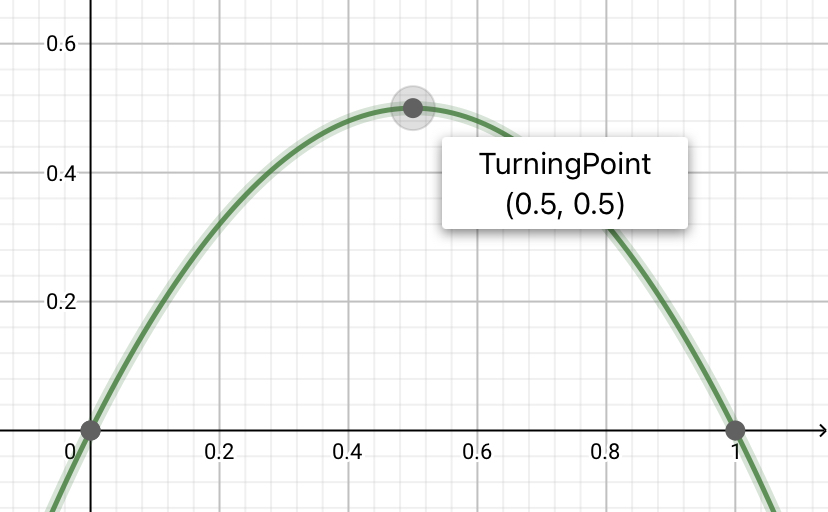
\includegraphics[width=0.5\textwidth]{coordinate_system_gini_index.jpeg}
\end{figure}

The optimal splits for the first iteration of the dataset look like the following. For numerical features the determination of 
the optimal split is more complex as for categorical ones because the calculation is not straight forward but must be computed
for every value in the value range to find the best overall split for a single feature. The example only shows the best splitting
criteria while a trial and error approach can be found in \ref{sec:appendix_dt}. 

Danceability: 
\begin{equation*}
    \begin{aligned}
        Gini^{left} &= 1 - ((\frac{2}{5})^2 + (\frac{3}{5})^2) = 0,48 
        \\
        Gini^{right}  &= 1 - ((\frac{3}{3})^2 + (\frac{0}{3})^2) = 0 
        \\
        G(Q_{0},\theta) &= \frac{5}{8} * 0,48 + \frac{3}{8} * 0 = 0,30
    \end{aligned}
\end{equation*}

Acousticness: 
\begin{equation*}
    \begin{aligned}
        Gini^{left}  &= 1 - ((\frac{4}{4})^2 + (\frac{0}{4})^2) = 0
        \\
        Gini^{right} &= 1 - ((\frac{1}{4})^2 + (\frac{3}{4})^2) = 0,36
        \\
        G(Q_{0},\theta) &= \frac{4}{8} * 0 + \frac{4}{8} * 0,36 = 0,18
    \end{aligned}
\end{equation*}

The conclusion is that the feature \emph{danceability} creates a bettter initial prediction than \emph{acousticness} does. It is thus 
determined to be the inital splitting criterion for the classification tree (figure \ref{fig:theory_first_split}). With the first iteration completed, the next iteration
will start with each leaf as its input. The second iteration will split the nodes further if no stop criterion is met. 

\begin{figure}[H]
    \centering
    \subfloat[\centering Decision Tree]{{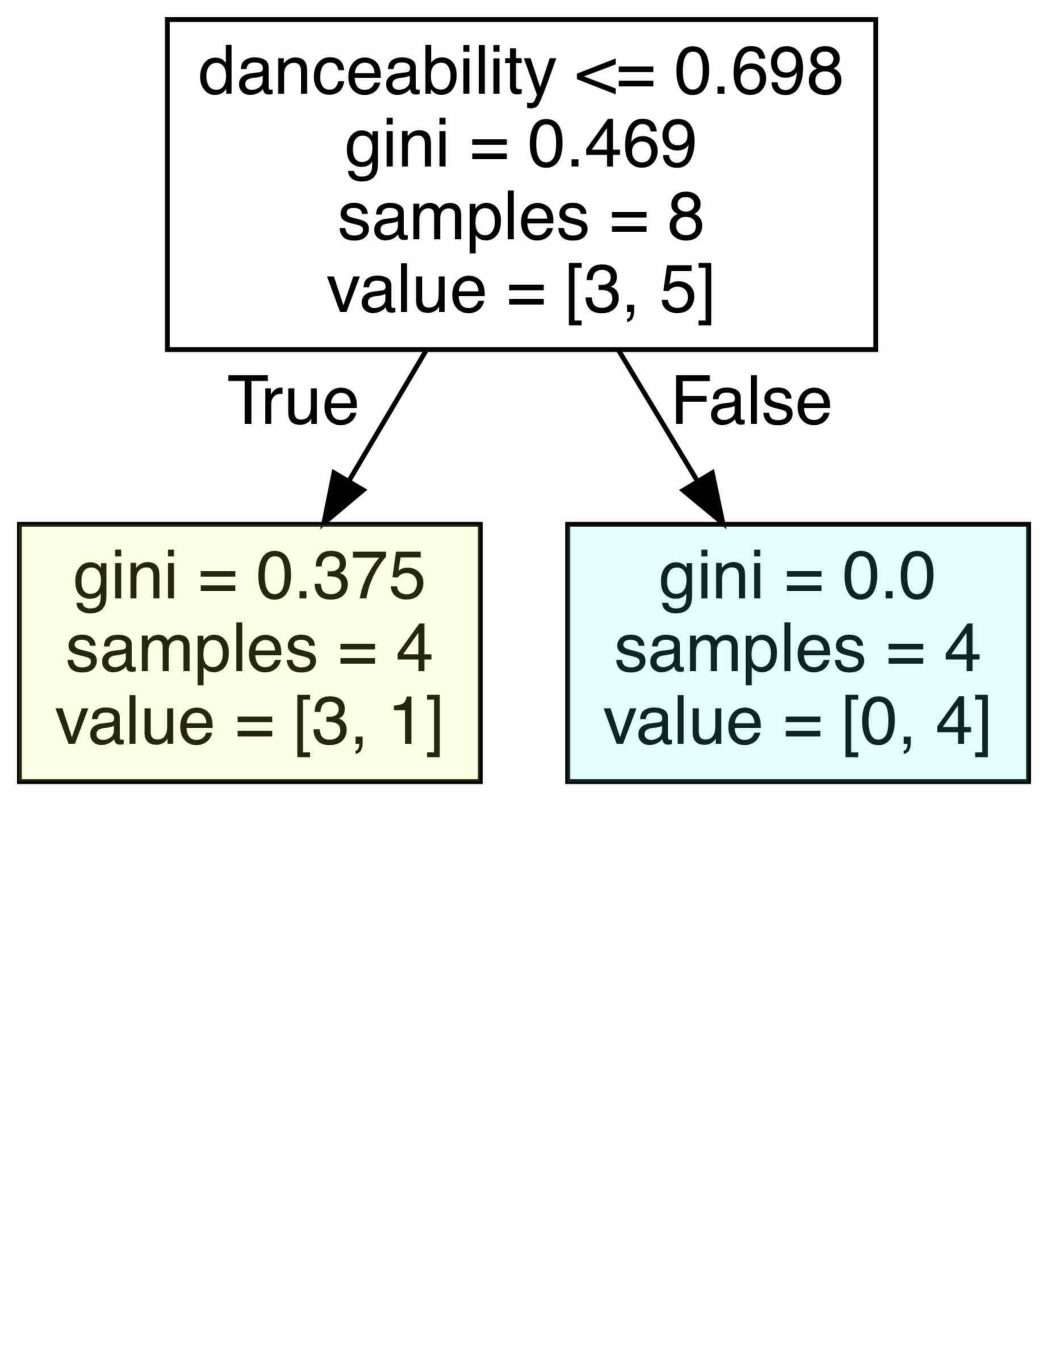
\includegraphics[width=6cm]{dt_first_split.svg.pdf} }}%
    \qquad
    \subfloat[\centering Classification Tree]{{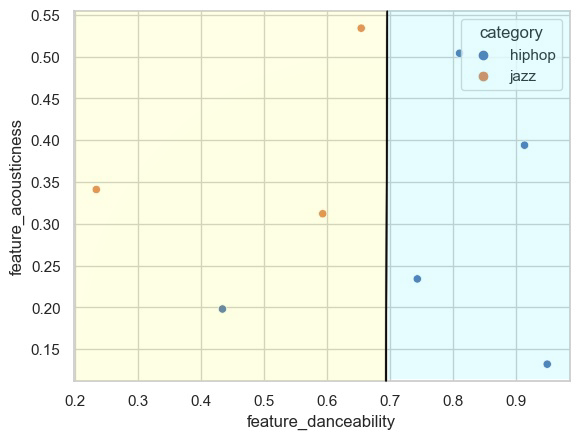
\includegraphics[width=6cm]{coordinate_system_id_first_split.png} }}%
    \caption{Decision tree first split}%
    \label{fig:theory_first_split}%
\end{figure}

\textbf{Stop Criteria:}

The natural stop criterion is a completely homogeneous data-group for a node. If a node only contains one single 
class of samples, no further splitting is possible. This is the case for the right node of the example marked in blue. The samples are completely
homogeneous and only consist of the category \emph{hiphop}. The node therefore automatically becomes a leaf and represents the 
category of samples. Other stop criteria can be predefined depending on own preference. The most relevant criterion is the 
definition of a maximum depth of the decision tree. Maximum depth describes a maximum amount of recurrent iterations before 
the algorithm automatically stops and treats the last nodes as leaves \cite[p.7]{lewis2000introduction}. Maximum depth belongs to a set of hyperparameters that
will be discussed in section \ref{sec:Modeling}.

\textbf{Completion of the example:}

The second iteration has both nodes created by the first iteration as its input but only the yellow node requires further splitting as 
the blue node is already fully classified. For the second iteration only the feature \emph{acousticness} is relevant as \emph{danceability} cannot 
split this subgroup of the dataset further. The input data for the second split looks like the following (table \ref{tbl:theory_input_data_second_step}) and the same calculation 
takes place again. 

\begin{table}[H]
    \centering
    \begin{tabular}{llrrr}
        \toprule
        category & track &  feature\_danceability &  feature\_acousticness &  label \\
        \midrule
          hiphop &    h5 &                 0.434 &                 0.198 &      1 \\
            jazz &    j1 &                 0.654 &                 0.534 &      0 \\
            jazz &    j2 &                 0.593 &                 0.312 &      0 \\
            jazz &    j3 &                 0.234 &                 0.341 &      0 \\
        \bottomrule
        \end{tabular}       
    \caption{Input data of second split}%
    \label{tbl:theory_input_data_second_step}%
  \end{table} 

  Acousticness: 
  \begin{equation*}
    \begin{aligned}
        Gini^{left} &= 1 - ((\frac{0}{1})^2 + (\frac{1}{1})^2) = 0
        \\
        Gini^{right}  &= 1 - ((\frac{3}{3})^2 + (\frac{0}{3})^2) = 0
        \\
        G(Q_{1},\theta) &= \frac{1}{4} * 0 + \frac{3}{4} * 0 = 0
\end{aligned}
\end{equation*}

This time \emph{acousticness} leads to two fully homogeneous subgroups and therefore marks the end of the classification tree as all samples are 
classified correctly. The second split looks like the following with the total classification tree displayed in figure \ref{fig:theory_second_split}.

\begin{figure}[H]
    \centering
    \subfloat[\centering Decision Tree]{{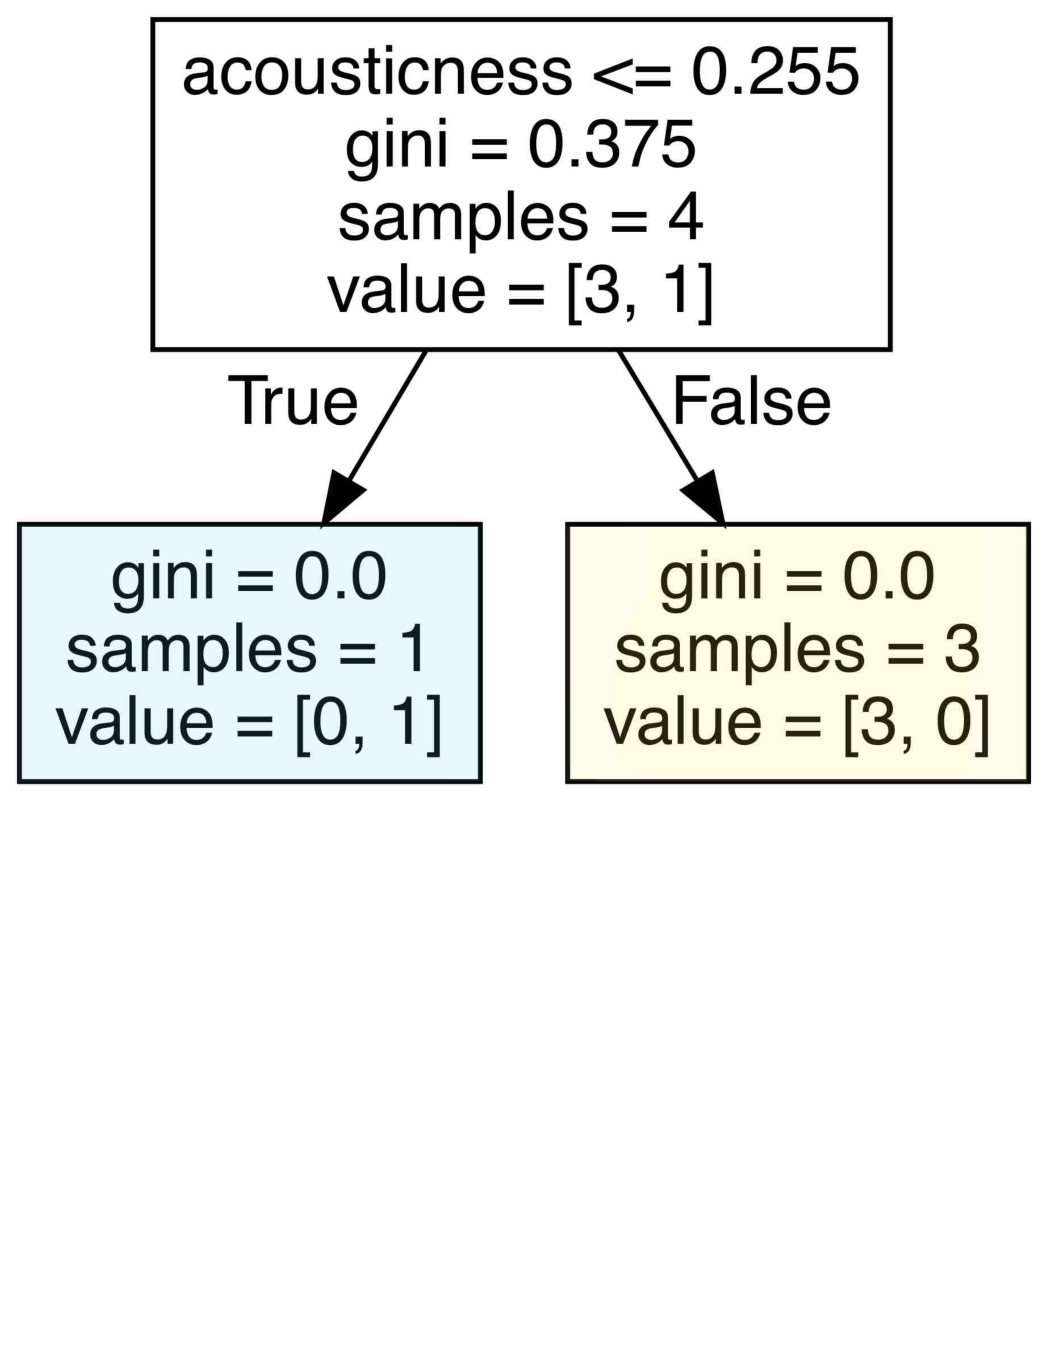
\includegraphics[width=6cm]{dt_second_split copy 2.svg.pdf} }}%
    \qquad
    \subfloat[\centering Classification Tree]{{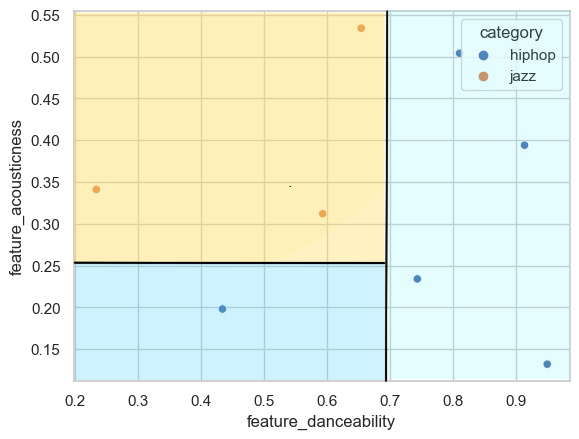
\includegraphics[width=6cm]{coordinate_system_id_second_split.png} }}%
    \caption{Decision Tree second Split}%
    \label{fig:theory_second_split}%
\end{figure}


\begin{figure}[H]
    \centering
    \caption[]{Final Classification Tree}
	\label{fig:dt_final_decision_tree}
    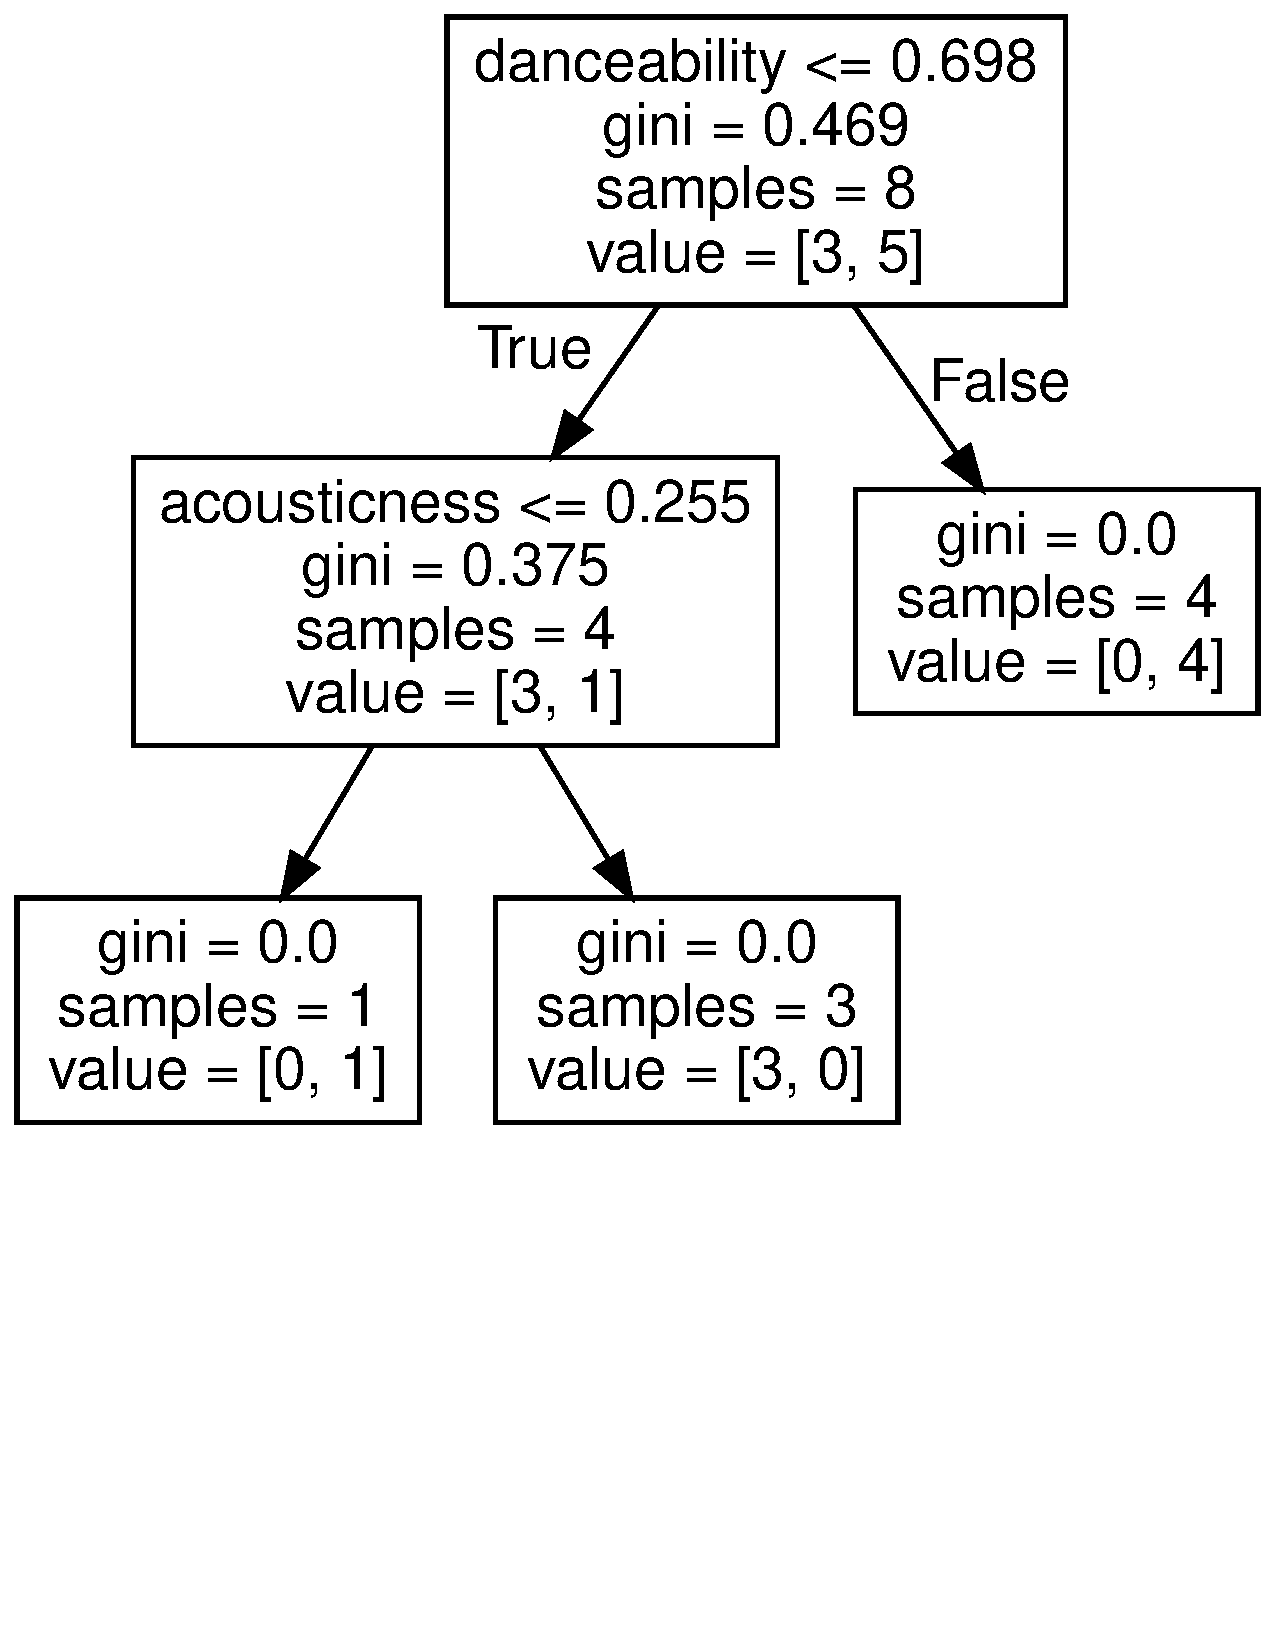
\includegraphics[width=0.58\textwidth]{dt_final_decision_tree.svg.pdf}
\end{figure}

%\textbf{Tree optimization:}
%
%Tree optimization plays a very relevant role because Trees often overclassify training data 
%without countermeasures \cite[p.7]{lewis2000introduction}. Although the training data is well classified, overfitted Decision 
%Trees often produce very poor results for test data. Too accurate classification of training 
%data can negatively affect Decision Trees, as they are less able to generalize the learned 
%knowledge. Pruning is a technique used to overcome overfitting problems by reducing the size of 
%Decision Trees \cite[p.331]{James2021}. Sections that provide little to no classification benefit are removed or not 
%constructed during the recursive splitting process. In essence, worse results for training data 
%are traded for better results for unknown data.

\subsubsection{Evaluation of Decision Trees}

In conclusion, decision trees can be assessed as follows. Starting with the advantages,
the main benefit is the overall simplicity of decision trees, both from a technical and 
business point of view \cite[p.339]{James2021}. For researchers and developers, trees are easy to construct, require little
to no data preparation, are almost universally applicable with the possibility of validation. 
However, the simplicity for business should not be underestimated either. When comparing machine
learning algorithms, the main comparison is often the accuracy of a model. The areas in which 
decision trees stand out include visualization and comprehensibility. The decision tree algorithm 
is a white box model that allows complete transparency and explainability \cite[10.10.]{scikit-decision_tree}. 

The disadvantages of decision trees are again closely related to their simplicity. Overfitting and 
the relative instability of decision trees are the main drawbacks and result in good memorization 
but a comparatively weak generalization ability \cite[p.340]{James2021} \cite[10.10.]{scikit-decision_tree}.

\subsection{Gradient Boosting}
\label{sec:Gradient Boosting}


The Gradient Boosting Algorithm is derived from \ac{GBM}, which are a family of 
powerful machine learning algorithms with a certain procedure pattern for the creation of models. 
In general, \acp{GBM} are very flexible in their characteristics with the possibility of utilizing 
multiple different Machine Learning algorithms as their foundation \cite{Natekin2013}.

Boosting differs from classical approaches as it does not consist out of a single predictive 
model but an ensemble approach. Ensemble algorithms contain multiple weak learners that form a 
committee to create a strong prediction. Weak learners are often very simple forms of traditional 
algorithms, like decision trees, and must just be able to predict parts of the dataset correctly. 
Only the combination of many weak learners allows the model to perform overall accurate 
predictions \cite{parr2022gb_explained_dtt} \cite[p.1f]{Buhlmann2004Bagging}. The most common form of ensemble algorithms are bagging algorithms with random 
forests as an example. Bagging, in essence, is the combination of multiple unique models. The 
prediction is formed by aggregating the outputs from all models into a single representative 
value. Typically, all models are derived from a single algorithm, like decision trees for random 
forests, but technically there is no limitation to aggregate outputs from different algorithms. 
Which is also true for other ensemble algorithms \cite[p.2]{Buhlmann2004Bagging}. 

Boosting, on the other hand, follows a different principle and does not rely on independent 
models with an aggregation function. Boosting fits new models sequentially and can thereby use 
earlier acquired knowledge for further iterations. This allows a GBM to train specific areas of 
the dataset where it has previously performed poorly \cite[p.11]{Buhlmann2004Bagging} \cite[p.345f]{James2021}.  

\subsubsection{Gradient Boosting Algorithm}
\label{sec:Gradient Boosting Algorithm}

The generic Gradient Boosting Algorithm follows a sequence of three steps beginning with the initialization of
the dataset, to the sequential training and ending with a final output. At the beginning, an 
additional initiation of the dataset and a loss function is necessary \cite{parr2022gb_explained_hrd}. The mathematical 
representation of the dataset is like the one used for decision tees. A summary: \(x_{i}\) represent the 
explanatory features while \(y_{i}\) represents the corresponding label for one data point of the input 
dataset \(N\) with a total number of \(n\) samples. 

The mathematical goal of the algorithm is to reconstruct the unknown functional dependance \(f\) 
between \(x_{i}\) and \(y_{i}\) with an estimate \(F^{*}\) for every data point, such that the specific loss 
function \(L(y, \gamma)\) is minimized (\ref{equ:gb_theory}) \cite[p.1189]{Friedman_2001} \cite[2.1]{Natekin2013}. 

\begin{equation}
    F^{*} = \arg \min_{\gamma} L(y,\gamma)
    \label{equ:gb_theory}
\end{equation}

\textbf{Loss Function and Weak Learners:}

The loss function is an indicator for the quality of the model. A small loss for a data point 
means that the prediction is close or identical to the observed label and the model therefore 
categorizes the sample correctly whereas a high loss implies that the model could not predict 
the sample well. Given a particular learning task and dataset, different loss functions must 
be considered as loss functions are only suitable for specific data and task constellations. The most common 
loss function for binary classification is the so-called bernoulli loss (\ref{equ:gb_bernoulli_loss}). The bernoulli loss 
can be transformed into a \(log(odds)\)-prediction (\ref{equ:gb_loss_function}) as it is better suited for further calculations \cite[3.1]{Natekin2013} \cite{bischl2022introduction_ml_bernoulli_loss}. 
Variations of (\ref{equ:gb_loss_function}) will be used in the following section to demonstrate the gradient boosting 
procedure.

\begin{equation}
    L(y_{m}, \gamma) = - log(likelihood)
    \label{equ:gb_bernoulli_loss}
\end{equation} 

\begin{equation}
    L(y_{m}, \gamma) = - y_{i} * log(odds) - log(1-p)
    \label{equ:gb_loss_function}
\end{equation}

Additionally, a machine learning algorithm must be defined as a weak learner. For \ac{GBM}s there 
are multiple learners to choose from. Again the choice mostly depends on the prediction 
task and available data \cite[3.2]{Natekin2013}. A classical approach is the use of Decision Trees, which was also 
chosen as the weak learner for this project. Decision Trees used for Gradient Boosting are 
always Regression Trees, regardless of whether they are used for regression or classification 
problems. The optimization parameters are almost identical to the ones of standalone Decision Trees, 
but the trees often look very different because they are specifically created as weak learners. 
As a result, the Decision Trees often only consist of very few layers with only 8-32 leaves.

\textbf{Initialization:}

To showcase the Gradient Boosting Algorithm the same sample dataset is used as for Decision Trees. 
It again consists of eight samples with two features and two categories as target labels. 

\begin{table}[H]
    \centering
    \begin{tabular}{llrrr}
        \toprule
        category & track &  feature\_danceability &  feature\_acousticness &  label \\
        \midrule
          hiphop &    h1 &                 0.949 &                 0.132 &      1 \\
          hiphop &    h2 &                 0.743 &                 0.234 &      1 \\
          hiphop &    h3 &                 0.913 &                 0.394 &      1 \\
          hiphop &    h4 &                 0.810 &                 0.504 &      1 \\
          hiphop &    h5 &                 0.434 &                 0.198 &      1 \\
            jazz &    j1 &                 0.654 &                 0.534 &      0 \\
            jazz &    j2 &                 0.593 &                 0.312 &      0 \\
            jazz &    j3 &                 0.234 &                 0.341 &      0 \\
        \bottomrule
        \end{tabular}        
    \caption{Input dataset}%
    \label{tbl:theory_input_data}%
  \end{table} 

The first step is to set an initial prediction for all samples of the dataset. The initial 
prediction is not unique for individual samples but a uniform value. The optimal initial 
prediction can be calculated using the following equation (\ref{equ:gb_initial_prediciton}) \cite[p.361]{Hastie_2009}. For \(F_{0}(x)\), representing the 
initial prediction, a minimum of \(\gamma \) is searched for. The right-hand side of the equation 
only consists of a sum for each sample \(i\) (of the total dataset \(N\)) of the known loss function 
with the respective label \(y_{i}\) and \(\gamma \) as its input. To find the low point of the equation, 
the derivate of the loss function is required. The final calculation of the overall \(log (odds)\) 
that a song is classified as \emph{hiphop} is the \(\log_{e}\) of the sum of songs of the category \emph{hiphop}
divided by the sum of the songs of the category \emph{jazz}. The result can be checked graphically 
as is equal to the \(x1\)-coordinate value of the low point of the \(log(odds)\)-prediction (figure \ref{fig:gb_turning_point-loss_function}). 

\begin{equation}
    F_{0}(x) = \arg \min_{\gamma } \sum_{i= 1}^{n} L(y_{i}, \gamma)
    \label{equ:gb_initial_prediciton}
\end{equation}

\begin{equation*}
    F_{0}(x) = \log_{e}(\frac{5}{3}) = 0.51
\end{equation*}

\begin{figure}[H]
    \centering
    \caption[]{Gradient boosting minimum for first prediction}
	\label{fig:gb_turning_point-loss_function}
    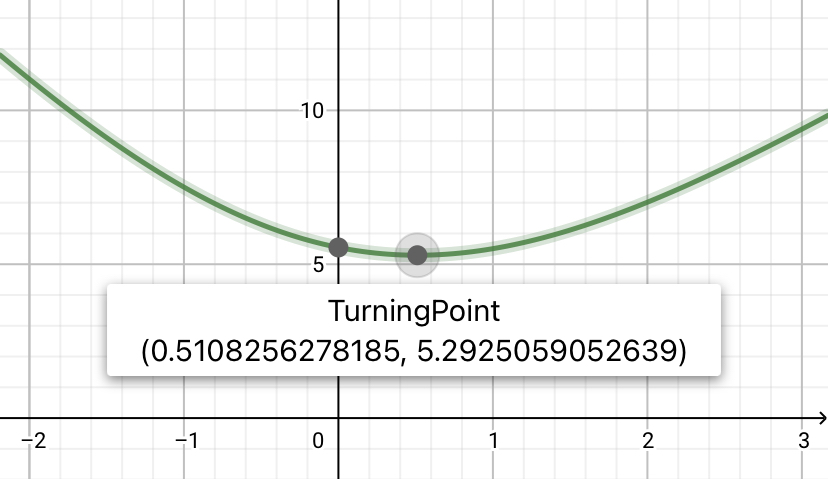
\includegraphics[width=0.5\textwidth]{TurningPoint-LossFunction.jpeg}
\end{figure}

\textbf{Sequential Processing:}

With the completion of the initialization of the dataset the modeling can begin. The training is a sequential 
process of constructing regression trees with a total of \(M\) iterations. The first iteration 
starts with \(m = 1\). The modelling consists out of four sub-steps which are numbered consecutively \cite[p.1198]{Friedman_2001}.

First, the \(log(odds)\)-prediction must be converted back into a probability \(p\) with the help of a 
logistic function as probability is easier to use for classification (\ref{equ:gb_prediction}). The result is 
that all songs have a \(63\%\) chance of belonging to the category \emph{hiphop}.

\begin{equation}
    p = \frac{e^{\log_{e}(odds)}}{1 + e^{\log_{e}(odds)}} 
    \label{equ:gb_prediction}
\end{equation}

\begin{equation*}
    p = \frac{e^{\log_{e}(\frac{5}{3})}}{1 + e^{\log_{e}(\frac{5}{3})}} = 0,63
\end{equation*}

In the \textbf{first step} the \acp{PR} \(r_{im}\) for each sample \(i\) of the dataset are created. The equation (\ref{equ:gb_redsiduals_theory}) 
for calculating the \ac{PR} consists out of known fragments. For every sample \(i\) a PR \(r_{im}\) 
is calculated using the derivative of the \(log(odds)\)-prediction with the label \(y_{i}\) and the 
prediction of the last iteration \(F = F_{m - 1}\) as its input \cite[p.361]{Hastie_2009}. Again, the equation can be 
simplified greatly. For each sample the \ac{PR} can be calculated by only 
subtracting the previously calculated probability \(p\) from the observed label \(y\) \cite{parr2022gb_explained_hrd} \cite{parr2022gb_explained_gbd}. Ideally, an additional 
column is created in which the PRs are temporarily stored (table \ref{tbl:theory_pseudo_residuals_1_iteration}). 

\begin{equation}
    \begin{aligned}
        r_{im} &= - (\frac{\partial L(y_{i}, F(x_{i}))}{\partial F(x_{i})})_{F = F_{m - 1}}
        \\
        r_{im} &= (y_{i} - p_{i})
        \label{equ:gb_redsiduals_theory}
    \end{aligned}
\end{equation}

This and every following calculation is explained for the track \emph{h1} of the dataset while the result for 
every other sample will be shown in form of a table. 

\begin{equation*}
r_{1,1} = 1 - 0.625 = 0.375
\end{equation*}

\begin{table}[H]
    \centering
    \begin{tabular}{llrrrr}
        \toprule
        category & track &  label & \(F_{0}(x)\) &  probability \(F_{0}(x)\) &  pseudo residuals \\
        \midrule
          hiphop &    h1 &      1 & 0.510826 &         0.624988 &            0.375012 \\
          hiphop &    h2 &      1 & 0.510826 &         0.624988 &            0.375012 \\
          hiphop &    h3 &      1 & 0.510826 &         0.624988 &            0.375012 \\
          hiphop &    h4 &      1 & 0.510826 &         0.624988 &            0.375012 \\
          hiphop &    h5 &      1 & 0.510826 &         0.624988 &            0.375012 \\
            jazz &    j1 &      0 & 0.510826 &         0.624988 &           -0.624988 \\
            jazz &    j2 &      0 & 0.510826 &         0.624988 &           -0.624988 \\
            jazz &    j3 &      0 & 0.510826 &         0.624988 &           -0.624988 \\
        \bottomrule
        \end{tabular} 
    \caption{Pseudo Residuals for first Iteration}%
    \label{tbl:theory_pseudo_residuals_1_iteration}%
  \end{table} 

The \textbf{second step} constructs the a Regression Tree out of the features from the samples with the corresponding 
PR as the label. For this example, only tree stumps are created to simplify the implementation. 
The regression tree for the first iteration is shown in figure \ref{fig:gb_1_regression_tree}. After the completion of the 
tree, terminal regions \(R_{jm}\) must be defined for every leaf. \(j\) starts with \(1\) and is increased for 
every leaf \cite[p.1195]{Friedman_2001}. 

\begin{figure}[H]
    \centering
    \caption[]{Regression tree for first iteration}
	\label{fig:gb_1_regression_tree}
    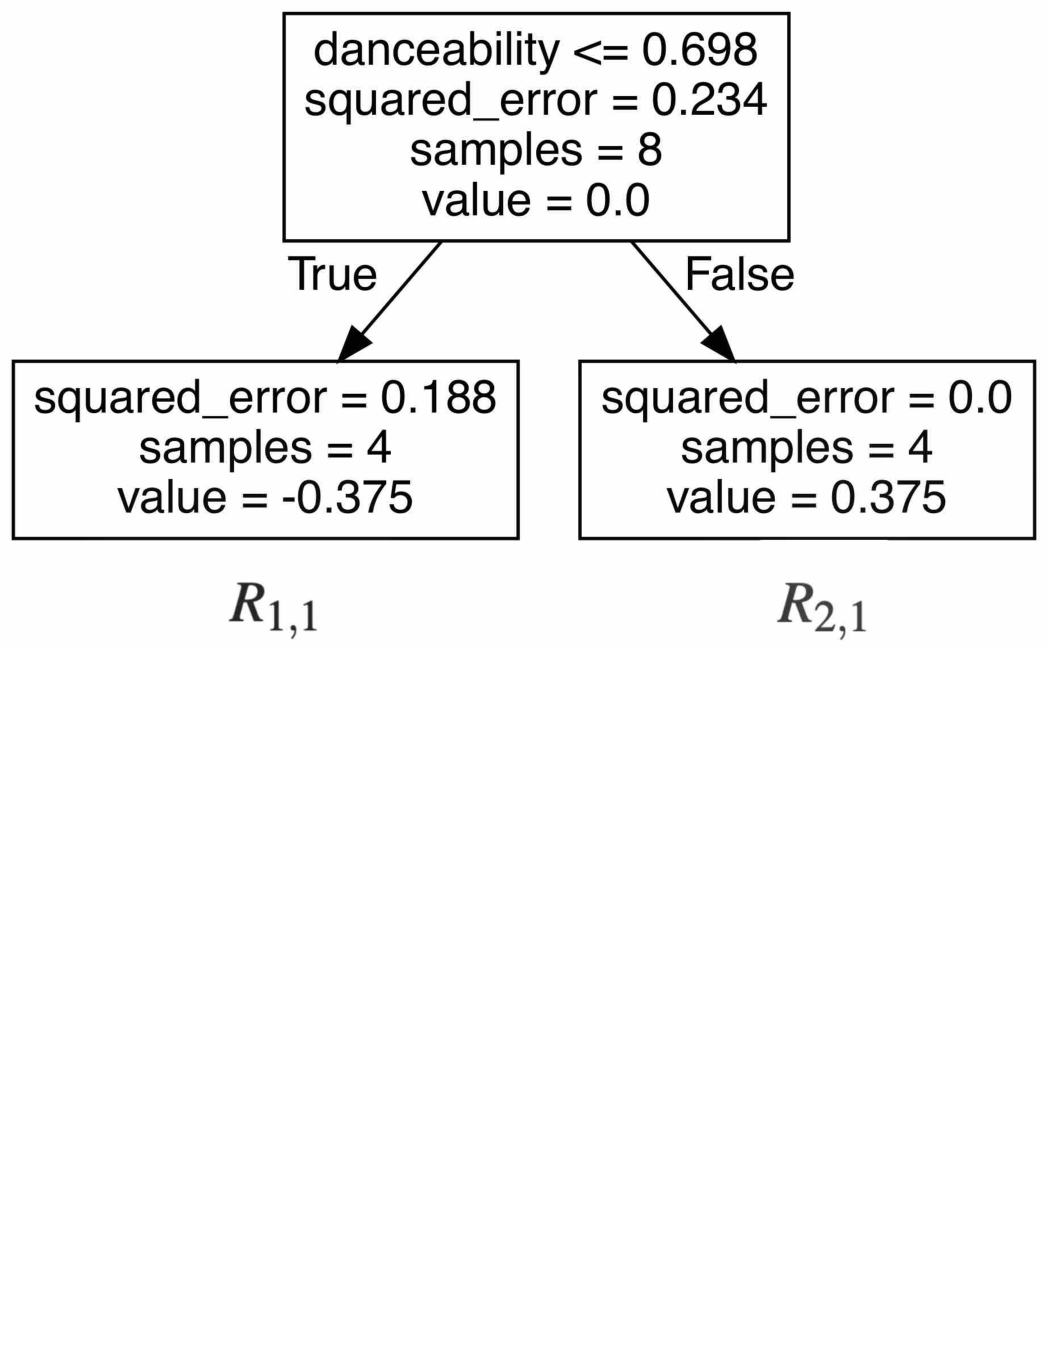
\includegraphics[width=0.5\textwidth]{gb_1_regression_tree.svg.pdf}
\end{figure}

In \textbf{step three}, following the completion of the regression tree, output values \(\gamma_{j, m}\) are calculated by using 
the equation presented in (\ref{equ:gb_output_value_theory}). For each leaf in the tree, \(\gamma_{j, m}\) is computed by finding 
\(\gamma_{j, m}\) that minimizes the loss function (11) \cite[p.361]{Hastie_2009}. Like in the initialization step, the derivative has 
to be created and set equal to \(0\). Again, after a complicated transformation, a very simple 
equation remains (11). The \(\gamma_{j, m}\)  can be calculated using only the \ac{PR} and the most 
recently predicted probabilities \(p\) for all samples in the leaf. 

\begin{equation}
    \begin{aligned}
        \gamma_{jm} &= \arg \min_{\gamma}\sum_{x_{i} \in R_{jm}} L(y_{i},F_{m-1}(x_{i}) + \gamma)
        \\
        \gamma_{jm} &= \frac{ \sum r_{im}}{\sum p_{i} * (1 - p_{i})}
        \label{equ:gb_output_value_theory}
    \end{aligned}
\end{equation}

For \(R_{2,1}\), which contains track \emph{h1}, the calculation looks like the following. Output values of the complete 
dataset are displayed in table 5.%\ref{tbl:theory_output_values_1_iteration}. 

\begin{equation*}
\gamma_{\;2,1} = \frac{0.375\;*\;4}{(\:0.625\;*\;(1\;-\;0.625))\;*\;4} = 1.6 
\end{equation*}

\begin{table}[H]
    \centering
    \begin{tabular}{llrrrr}
        \toprule
        category & track &  label &  \(F_{0}(x)\) &  pseudo residuals &  output value \\
        \midrule
          hiphop &    h1 &      1 & 0.510826 &            0.375012 &        1.600032 \\
          hiphop &    h2 &      1 & 0.510826 &            0.375012 &        1.600032 \\
          hiphop &    h3 &      1 & 0.510826 &            0.375012 &        1.600032 \\
          hiphop &    h4 &      1 & 0.510826 &            0.375012 &        1.600032 \\
          hiphop &    h5 &      1 & 0.510826 &            0.375012 &       -1.599926 \\
            jazz &    j1 &      0 & 0.510826 &           -0.624988 &       -1.599926 \\
            jazz &    j2 &      0 & 0.510826 &           -0.624988 &       -1.599926 \\
            jazz &    j3 &      0 & 0.510826 &           -0.624988 &       -1.599926 \\
        \bottomrule
        \end{tabular}
    \caption{Output values for first iteration}%
    \label{tbl:theory_output_values_1_iteration}%
  \end{table} 

\textbf{Step four} marks the end of the first iteration and creates a new prediction \(F_{m}(x)\) for each sample. 
The new \(log(odds)\)-prediction is based on the last \(log(odds)\)-prediction plus the learning rate \(\nu\) multiplied by 
the output values for the sample of the last regression tree (\ref{equ:gb_new_prediction_theory}) \cite[p.1203]{Friedman_2001}. Normally, there is only one 
output value for a sample which makes the summation sign obsolete. The learning rate \(\nu\) is a 
hyperparameter for gradient boosting. For this example, a high \(\nu\) of \(0.6\) is used to better visualize 
the changes. In practice a \(\nu \) in the order of \(0.1\) is common as a small learning rate tends to
give better results but also requires much more iterations \cite[p.1206]{Friedman_2001}. 

\begin{equation}
    F_{m}(x) = F_{m}(x- 1) + \nu * \sum_{j = 1}^{J_{m}} \gamma_{jm}I(x \in R_{jm})
    \label{equ:gb_new_prediction_theory}
\end{equation}

The prediction \(F_{1}(x)\) for \emph{h1} is shown below while the complete dataset is again displayed in table \ref{tbl:theory_output_values_1_iteration} with also 
the probabilites shown. As one can see, the probabilites for most samples got closer to the label. However, for track
\emph{h5} the prediction got worse. This is why multiple iterations are necessary to form a well-founded prediction.

\begin{equation*}
F_{1}(x) = 0.51 + 0.6 * 1.6 = 1.47
\end{equation*}


\begin{table}[H]
    \centering
    \begin{tabular}{llrrrrr}
        \toprule
        category & track &  label & \(F_{0}(x)\) &  probability \(F_{0}(x)\) &  \(F_{1}(x)\) &  probability \(F_{1}(x)\) \\
        \midrule
          hiphop &    h1 &      1 & 0.510826 &         0.624988 &  1.470845 &         0.813163 \\
          hiphop &    h2 &      1 & 0.510826 &         0.624988 &  1.470845 &         0.813163 \\
          hiphop &    h3 &      1 & 0.510826 &         0.624988 &  1.470845 &         0.813163 \\
          hiphop &    h4 &      1 & 0.510826 &         0.624988 &  1.470845 &         0.813163 \\
          hiphop &    h5 &      1 & 0.510826 &         0.624988 & -0.449130 &         0.389579 \\
            jazz &    j1 &      0 & 0.510826 &         0.624988 & -0.449130 &         0.389579 \\
            jazz &    j2 &      0 & 0.510826 &         0.624988 & -0.449130 &         0.389579 \\
            jazz &    j3 &      0 & 0.510826 &         0.624988 & -0.449130 &         0.389579 \\
        \bottomrule
        \end{tabular}
    \caption{Gradient boosting complete}%
    \label{tbl:theory_output_values_1_iteration}%
  \end{table} 

The second iteration of the modelling phase follows the exact same principles and will again be showcased for track \emph{h1}. 
It marks the end for this example. 

\begin{itemize}

    \item New probability:

    \begin{equation*}
        p = \frac{e^{1.47}}{1 + e^{1.47}} = 0,81
    \end{equation*}

    \item New pseudo residuals: 

    \begin{equation*}
        r_{1, 2} = 1 - 0.81 = 0.19
    \end{equation*}
    
    \item New Decision Tree with terminal regions (figure \ref{fig:gb_2_regression_tree})

    \item New output value: 

    \begin{equation*}
        \gamma_{\;2,2} = \frac{0.98}{0.54} = 1.81 
    \end{equation*}

    \item New prediction:

    \begin{equation*}
        F_{2}(x) = 1.47 + 0.6 * 1.81 = 2.56
    \end{equation*}

    \item New probability:

    \begin{equation*}
        p = \frac{e^{2.56}}{1 + e^{2.56}} = 0.93 
    \end{equation*}

\end{itemize}

\begin{figure}[H]
    \centering
    \caption[]{Regression Tree for second Iteration}
    \label{fig:gb_2_regression_tree}
    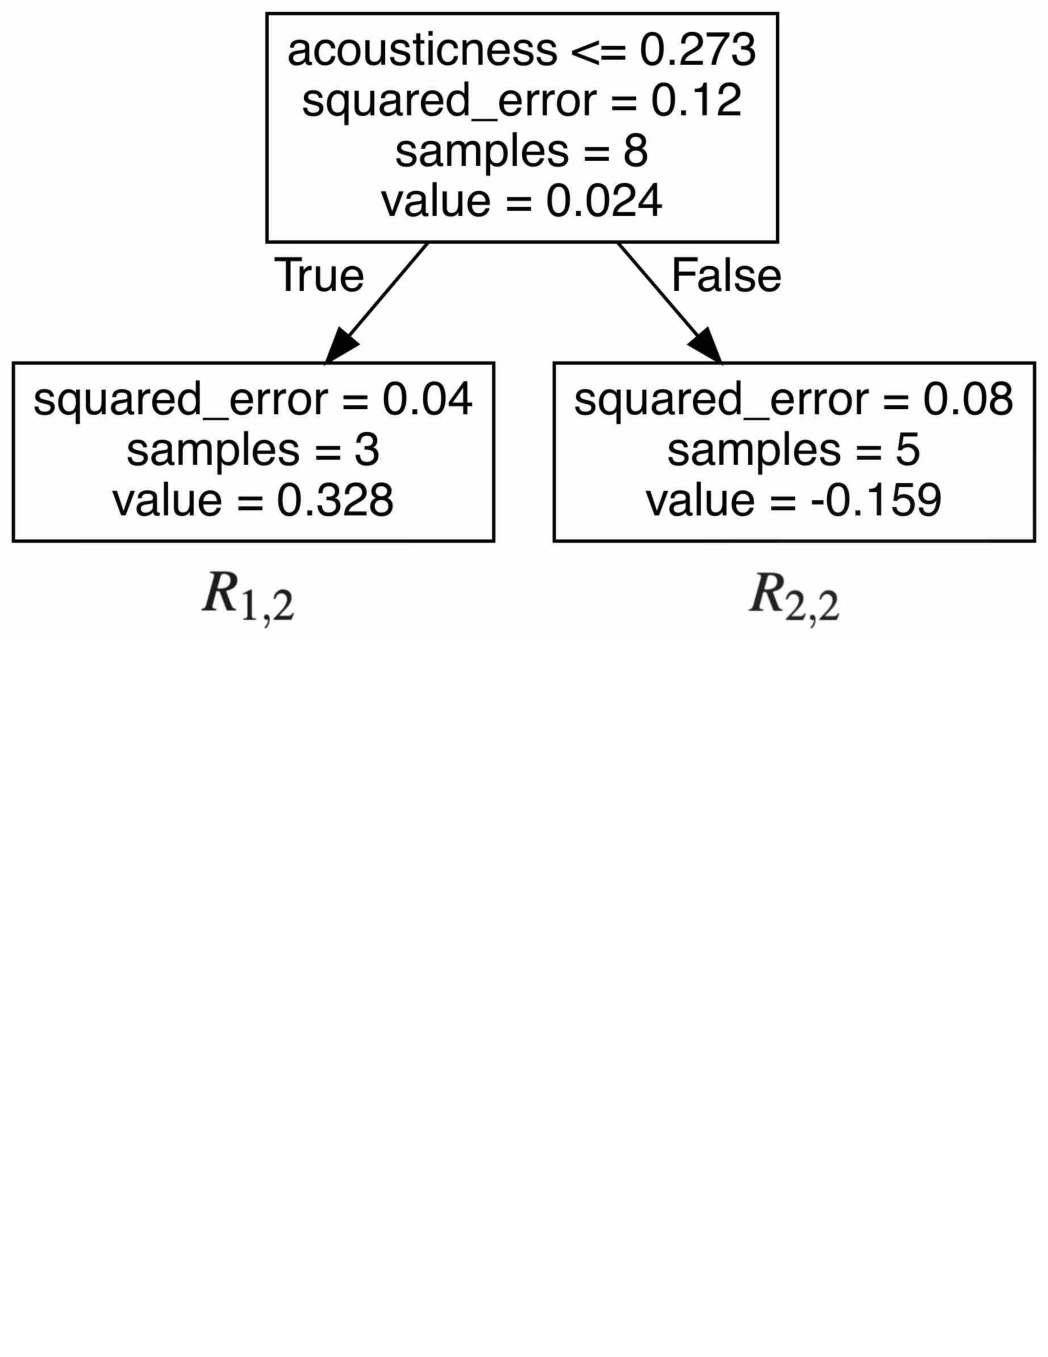
\includegraphics[width=0.5\textwidth]{gb_2_regression_tree.svg.pdf}
\end{figure}

The iterative modeling is repeated until \(M\) is reached. \(M\) marks the completion of training for the Gradient 
Boosting model. \(F_{M}(x)\) is the final prediction for every sample. Lastly, the predictions
must again be transformed to probabilites like for the calculation of the \ac{PR}. For the final probabilities, 
thresholds are used to compute the category to which the samples belong \cite[p.1204]{Friedman_2001}. A typical threshold 
for binary classification is \(0.5\) as it splits \(F_{M}(x)\) into two equal classes.

\textbf{Output:}

Sample \emph{h1} has a final probability \(0.93\) of belonging to the category \emph{hiphop}. \(0.93\) is by far greater than the 
predefined threshold of \(0.5\) and thus \emph{h1} is classified as a track that belongs to the category \emph{hiphop}. Table \ref{tbl:theory_gb_final_output} shows
that all samples are classified correctly but some less clear than others. A real-world implementation would consist 
out of more iterative models with different regression trees and a different learning rate to enhance the 
classification potential. Also the dataset would be very different with more samples that consist out of more features. 

\begin{table}[H]
    \centering
    \begin{tabular}{llrrrrr}
        \toprule
        category & track &  prob. \(F_{0}(x)\) &    \(F_{1}(x)\) &  prob. \(F_{1}(x)\) &       \(F_{2}(x)\) &  Output Probability \\
        \midrule
          hiphop &    h1 &         0.624988 &  1.470845 &         0.813163 &  2.560923 &                          0.928286 \\
          hiphop &    h2 &         0.624988 &  1.470845 &         0.813163 &  2.560923 &                          0.928286 \\
          hiphop &    h3 &         0.624988 &  1.470845 &         0.813163 &  1.001911 &                          0.731414 \\
          hiphop &    h4 &         0.624988 &  1.470845 &         0.813163 &  1.001911 &                          0.731414 \\
          hiphop &    h5 &         0.624988 & -0.449130 &         0.389579 &  0.640948 &                          0.654953 \\
            jazz &    j1 &         0.624988 & -0.449130 &         0.389579 & -0.918064 &                          0.285372 \\
            jazz &    j2 &         0.624988 & -0.449130 &         0.389579 & -0.918064 &                          0.285372 \\
            jazz &    j3 &         0.624988 & -0.449130 &         0.389579 & -0.918064 &                          0.285372 \\
        \bottomrule
        \end{tabular}           
    \caption{Gradient boosting Final Output}%
    \label{tbl:theory_gb_final_output}%
  \end{table} 

An unknown sample gets initialized by \(F_{0}(x)\) and is sequentially routed through every model. For each iteration the 
prediction is updated using the output value of the regression tree. Finally, the last probability is used to classify 
the sample using the predefined threshold. 

\subsubsection{Evaluation of Gradient Boosting}

Gradient Boosting is a very powerful method as it can effectively capture complex dependencies for various machine 
learning problems. \ac{GBM}s improve many existing algorithms, such as decision trees, because many problems associated 
with single large models are (partially) solved by the iterative ensemble approach.

The main benefit over Decision Trees is the stability of Gradient Boosting. While large trees always have to make tradeoffs 
between detail and overcategorization, Gradient Boosting can successively get to deeper levels of detail thanks to 
small trees with overall better generalization. Furthermore the flexbility of Gradient Boosting and boosting in general is massive 
as it only represents the framework with many parameters to adapt the algorithm very specifically to the usecase \cite[7.2]{Natekin2013}

The drawbacks of Gradient Boosting often arise in practice. Gradient Boosting has a significantly higher memory consumption and 
build time, because the model must be constructed sequentially. Also the evalutation is more time consuming as the sample must be processed 
by each model. From a business perspective Gradient Boosting also has disadvantages. While the overall prediction is better, it is
more complex to evaluate and explain \cite[7.2]{Natekin2013} \cite[p.27]{Buhlmann2004Bagging}. 
\subsection{Concepts in Data Preparation and Modeling}

In this section, concepts and processes, which are applied during
data preparation and modeling, are discussed theoretically.
The practical implementation is shown in sections \ref{sec:Data Preparation} and \ref{sec:Modeling}.

\subsubsection{Mean Removal, Variance Scaling and Standardization}
\label{sec:Mean Removal, Variance Scaling and Standardization}
During the data preparation stage of model development, it can be helpful to transform the data into a different shape
to improve the results of a model.\cite[35]{Subasi2020} This subsection explains some methods of data transformation, which are used in the
implementation section.

\textbf{Mean Removal} means shifting the data in a column, so that the mean $\overline{x}$ of all datapoints in the
column is equal to $0$.\cite{ScikitPreprocessing}
An example set of integers $a_1 = \{6, 7, 2, 1\}$ has a mean of $\overline{x_1} = 4$.
Removing it's mean without distorting other properties of the data entails subtracting $4$ from each member of the
set, resulting in a new set $a_2 = \{2, 3, -2, -3\}$ with $\overline{x_2} = 0$. The dataset is now centered around $0$.

\textbf{Variance Scaling} involves transforming the data in a way, that each column has unit variance, meaning variance
$\sigma^2 = 1$.\cite{ScikitPreprocessing} This is done by dividing each member of the column by the column's standard deviation.
An example set of integers $b_1 = \{6, 7, 2, 1\}$ has standard deviation $\sigma_1 = 2.94$ and variance $\sigma_1^2 = 8.67$.
Dividing each member of $b_1$ by $\sigma_1$ results in the set $b_2 = \{2.04, 2.38, 0.68, 0.34\}$ with variance $\sigma_2^2 = 1$.

\textbf{Standardization} involves performing both mean removal and variance scaling on a column.\cite{ScikitPreprocessing}
Standardizing an example set $c_1 = \{6, 7, 2, 1\}$ would result in the following set $c_2 = \{0.68, 1.02, -0.68, 01.02\}$.
Standardized features are normally distributed. Many machine learning have improved results when receiving standardized input
data. It has the additional benefit of equalizing the impact of features while keeping valuable information about the outliers
and value range.\cite[35]{Subasi2020}

\subsubsection{Dimension Reduction}
\label{sec:Dimension Reduction}

Dimension reduction refers to reducing the number of dimensions, so the number of
features in the input data, while keeping the highest possible amount of information from
the original dataset. The benefit of this is, that some features might not contribute to a better model,
but instead promote bias and overfitting.
%With dimension reduction, the smallest amount of features,
%which offers the highest ability of generalization is attempted to be found.
There are multiple ways to reduce dimensions, such as feature selection, where some features, which don't
contribute to a better model, are simply removed.
New features can be constructed by using data from different original features and
combining it into one, also reducing the dimensionality.
Another approach is \ac{PCA}. Here features are constructed by finding
principal components in a dataset. This is done by denoting the data in m-dimensional space,
where each feature is contained in one spatial dimension.
The first principal component is found by rotating the feature space to find the direction
which offers the highest variance in the whole dataset.
The second component must be orthogonal to the first one and again have the highest variance
of all possible directions. This can be repeated to create as many principal components as are benefitial to the model.
Dimension Reduction using \ac{PCA} was attempted as part of this project,
but is not explained deeper as it didn't yield great result for this dataset.

\subsubsection{Hyperparameter Optimization}

Machine learning models have two types of parameters: model parameters and hyperparameters.
Model parameters are values, which are optimized using training data during the training process.
They are not specified in advance.
Hyperparameters on the other hand are not optimized using data, but are specified before training.
They are like "settings" for the estimator. 
\textbf{\{Add example for decision trees\}}

Hyperparameters are not optimized during training, but still influence the results of a model.
There are multiple ways to find the best set of hyperparameters.
In this project, grid search is used, which takes a parameter grid containing
multiple values for each hyperparameter as input.
A model is trained using every possible combination of all given values on the grid and a score
is calculated for each model. The best combination of hyperparameters are the ones used on the model
with the highest score. This might not be the optimal set of hyperparameters though, as only values
in the search grid are considered.

\subsubsection{k-fold Cross Validation}

When training a model, it is necessary to split the data into train and test samples.
Using the same data for training and calculating the accuracy
score of a model would result in a model, that is fitted exactly to the training
data. It will perform very well on that data, but will fail to make predictions on any data
it has not yet seen. This is called overfitting.

When optimizing the hyperparameters of an estimator, one could use the test set to score
the model and find the best parameters. A problem with this approach is, that now test data,
which should be completely independent from the training process,
is involved in the optimization process, which could lead to the hyperparameters being
"fitted" to the test data.

Cross validation is a solution to this problem during optimization, the training set is
split into $k$ groups, named folds. A given estimator is trained on $k-1$ folds and its accuracy
is calculated using the samples in the remaining folds. This is done $k$ times, using a different fold
for scoring each time. The average of all scores is the cross-validation score, giving a good
representation of the overall performance of the estimator.
The benefit of this is, that test data is kept completely seperate from training data, but there
is still a good way of evaluating the performance of an estimator trained with a given set
of hyperparameters. This is crucial during hyperparameter optimization, as the best parameters
can not be found without a good way to score each model.


\subsection{Cross Industry Standard Process for Data Mining}

The CRISP-DM Reference Model is an organizational model for data mining projects and provides
an overview of the life cycle of such projects.  
The life cycle of a data mining project is divided into six phases: Business Understanding,
Data Understanding, Data Preparation, Modeling, Evaluation and Deployment. 
The order of the phases is not strictly adhered to. In certain projects,
the outcome of each phase determines which phase or which specific task in a phase must be performed next.
However, the process of data mining is to be understood more as a part of the process.
This means that data mining is not necessarily complete once a solution is implemented. 
The lessons that emerge during the process and from the solution can raise new,
often more focused business questions. 
Subsequent data mining processes can benefit from, and often build on,
the lessons learned from previous processes.

Firstly, in the step of Business understanding, an in-depth analysis of the business -objectives and -needs has to be done. 
From these insights, the current situation must be accessed and the goals of carrying out the processes must be defined. 
Following with Data Understanding, data is now collected in a targeted or untargeted manner. 
The collected data can be table entries, answers from questionnaires, sequence recordings from machines and so on. 
As a result, the relevant data must be pulled together and made accessible. Additionally, data understanding contains checking the quality of the data.
With unsufficient, or bad data, the model may produce bad or even wrong outcomes.
After the sources are completely identified, proper selection, cleansing, constructing and formatting is done in the step of Data Preparation. 
The data cleaning and quality assurance of the data within the data exploration is the most costly phase of the project. 
It will usually also require the largest share of the available project time, but it is crucial. Here, possible anomalies in the data structure as well as data errors can be identified in advance. 
This phase has a decisive influence on the quality of the overall result. 

When it comes to Modeling, the appropriate analytical procedure is chosen to generate predictions and groupings. Connections and structures in the data are also visualized. 
It is important to present these in such a way that the most meaningful visualizations possible are created, which allow the company to make decisions based on evidence-based data.
During the Step of Evaluation, the results of models are evaluated in the backdrop of business intentions. 
Then new objectives may sprout up owing to the new patterns discovered. This is, in fact, an iterative process and the decision whether to consider them or not has 
to be made in this step before moving on to the final phase. 
The creation of the model is generally not the end of the project. Typically, the knowledge gained must be organized and presented in a way that the customer can use. 
Depending on the requirements, the deployment phase can be as simple as creating a report or as complex as implementing a repeatable data mining process. 
\subsection{Application Programming Interfaces}

This section gives an overview over the basic concepts and technologies behind Web \acp{API}.
An \ac{API} in general is an interface between two pieces of software.\cite[S.1]{reddy2011api}
These might run on the same machine and communicate locally, in the case of a desktop application for example,
or on seperate machines that are connected via some network, e.g. in a client/server application.
An API is a construct, which abstracts complex functionality away and provides a simple interface
to interact with and benefit from the complex structures behind the API.\cite{Mozilla}
This section focuses specifically on Web APIs, which is a form of API that can be accessed over the internet
using the HTTP protocol.\cite{StoplightAPITypes}

APIs are used in this project in the context of data collection and the fundamentals explained in this section
are needed to understand section \ref{sec:Data Collection}.

\subsubsection{The HTTP Protocol}

All communication on the world wide web is conducted through \ac{HTTP},
because it is reliable and guarantees data integrity and prevents the destruction or distortion
of data during transit\cite[3f.]{gourley2002http}

Most communication on the Web is conducted between a client and a server. The client usually
requests a resource from the server and the server responds with that resource, which the client
can then use\cite[4]{gourley2002http}. As these resources could have a number of datatypes, e.g.
an HTML page, a JPEG image or JSON objects, every message has a specific MIME type,
which is used to inform the receiver, which type of data is contained in the message.
The receiver (usually the client) can then handle the data appropriately, depending on it's type.\cite[5f]{gourley2002http}

When a client requests a ressource, it must tell the server what specific resource it wants to
have. A resource can be uniquely identified using a \ac{URL}.
Figure \ref{fig:Description of different parts of a URL} shows how URLs are structured.
It starts with the protocol to be used, which tells the server, how the communication should commence.
Next the host is specified, usually in form of a domain. It refers to a specific
server or a group of servers which have the resource or know where to find it.
After the domain, the path to the requested resource is given.\cite[6f., 24]{gourley2002http}
If the server knows where to find the resource and the client is authorized to see it,
the server will send it to the client.
In the context of APIs, a URL pointing to a specific resource is also called an "API endpoint".\cite{Cooksey2014}
This interaction between client and server is usually done in an HTTP transaction.

\begin{figure}[H]
    \caption{Description of different parts of a URL}
	\label{fig:Description of different parts of a URL}
    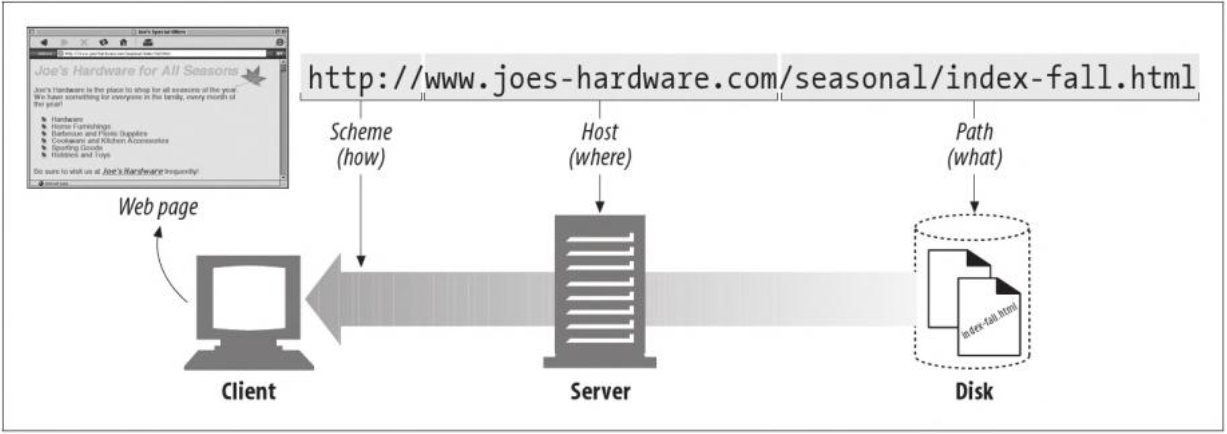
\includegraphics[width=1\textwidth]{URLDescription}
    \\
    Source: \cite[24]{gourley2002http}
\end{figure}

A transaction consists of a request (sent from client to server) and a response in which the
server answers the clients request in some way.\cite[8]{gourley2002http}
In the context of Web APIs, a request made to an API is also called "API call".\cite{StoplightAPITypes}
Figure \ref{fig:Example HTTP request and response messages} shows the structure of an 
HTTP request and response message.

\begin{figure}[H]
    \caption{Example HTTP request and response messages}
	\label{fig:Example HTTP request and response messages}
    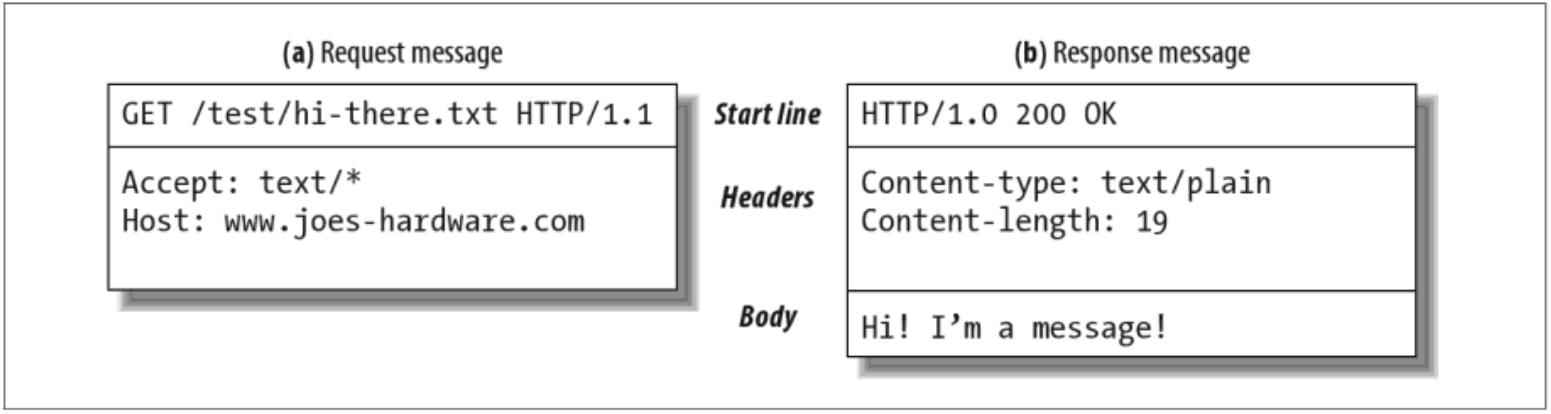
\includegraphics[width=1\textwidth]{HTTPMessageExample}
    \\
    Source: \cite[47]{gourley2002http}
\end{figure}

Every HTTP request message has a start line.
It contains a method, which tells the server what action to perform on the resource, the URL
and some protocol information.\cite[47]{gourley2002http}
After the start line, some headers are given. These contain information about the request,
e.g. what types of data the client can accept or credentials for authorization.
Some requests also contain a body to give some data to the server. \cite[52]{gourley2002http}

A response message also starts with a start line, although it does not contain a method or URL
Instead it contains protocol information and status information in the form of a numerical
status code and status text.\cite[48]{gourley2002http}
A response also contains headers and might contain a body.\cite[52]{gourley2002http}

There are many HTTP methods defined, that can be used to delete a resource, store
data on the server, get header information for a document and more.\cite[48]{gourley2002http}
In this paper, only two HTTP methods are used, GET and POST.
It is used to ask the server to send a resource to the client.
A GET request message is used to ask the server to send a resource to the client.
It does not contain a body.\cite[48]{gourley2002http}
A POST request message is used to send data to the server for processing. The data to be
processed is sent in the request body.\cite[48]{gourley2002http}

There are also many status codes defined, which tell the client the status of the transaction.
This is necessary, because the client's request can not always be fulfilled successfully
by the server.\cite[49]{gourley2002http}
The server might not be able to find the server, he might not be able to store
the data or the client might not have given the right authorization credentials to perform the
requested action. For each of these problems, there are predefined status codes.
For example, codes in the range 200-299 represent success, codes from 400-499 tell the client
that his request contained an error and 500-599 are used to inform about an error which happened on
the server.\cite[49]{gourley2002http}
Table \ref{tbl:Common status codes} shows some common status codes. There are many other
status code defined in the standard, but they are not relevant for this paper.

\begin{table}[H]
 \caption{Common status codes}
 \label{tbl:Common status codes}
\begin{tabular}{|| c | c | c ||} 
 \hline
 Status code & Reason phrase & Meaning \\ [0.5ex]
 \hline\hline
 200 & OK & Successful transaction. Any requested data is in the response body \\ [1ex]
 \hline
 401 & Unauthorized & The response needs to contain credentials to access the requested resource. \\ [1ex]
 \hline
 404 & Not Found & The server cannot find a resource for the requested URL. \\ [1ex]
 \hline
\end{tabular}
Source: \cite[50]{gourley2002http}
\end{table}

There are also many different headers defined in the HTTP standard.
Some that are important for this paper:

\begin{itemize}
    \item Authorization: Request header, which contains the credentials the client is using to authenticate.
    This might be username and password or a token.
    \item Content-Type: The datatype of the data contained in the body
\end{itemize}

\subsubsection{JSON}

Most modern APIs transmit data to the client using \ac{JSON}.
It is a text-based format able to represent structured data. \cite{MozillaJSON}
It is easy for humans to read and write JSON objects, but is also easily processed by computers.
JSON is tightly integrated in the JavaScript programming language and can be used without any parsing or serialization.\cite{OracleJSON}
This is beneficial, as JavaScript is widely used both on the client and server side of web applications. 
JSON can also be used with many other programming languages. \cite{JsonOrgIntroduction}

JSON supports only six very basic datatypes: String, Number, Boolean, Null, Object and Array.\cite{OracleJSON}
The following code snippet shows how each of the datatypes are defined in JSON.

\begin{lstlisting}[language=JavaScript]
    {
        "string": "Martin",
        "number": 200,
        "number2": 300,
        "boolean": true,
        "booleanFalse": false,
        "nullValue": null,
        "object": {
            "objectAttribute": "string",
            "objectAttribute2": "string2"
        },
        "array": [
            "entry1",
            "entry2",
            {
                "objectInArray": true
            }
        ]
    }
\end{lstlisting}

The code snippet shows, that the whole JSON object is wrapped in curly braces.
Each attribute is defined as a attribute-value-pair, where the attribute name is defined in 
double quotes, followed by a colon and the value definition. String values are defined in 
double quotes, numbers and booleans without. Objects are defined in curly braces and can
again contain any datatype.
Arrays are defined using brackets. They can contain any number of entries of any type.
Types can also be mixed within the same array.
All attributes-value-pairs or array items are seperated by commas.
Indentation and newline characters are not parsed in JSON as all syntax is given using
the characters '"{}[]:,'.\cite{JsonOrgIntroduction}

The MIME type of a JSON object is called "application/json".
An HTTP response containing JSON data will therefore always have the header
"Content-Type: application/json".\cite[Chapter 2]{richardson2008restful}

The text-based nature, good readability, simplicity and easy parsing and processing are reasons
for the wide usage of the data format. \cite{OracleJSON}
JSON is also used by the Spotify API to transfer data to the client.\cite{SpotifyWebAPI}

\subsubsection{Types of Web APIs}

As previously mentioned Web APIs are accessed through the HTTP protocol\cite{StoplightAPITypes}.
and offer a way for applications and data servers to communicate and exchange 
data over the web.\cite{Lane2019WhatIs}
They are used to power desktop, web and mobile applications. pass data between different
services, systems and devices. They make automated data access and retrieval possible
and enable the integration of internal and external systems into processes and data flows.\cite{Lane2019WhatIs}

There are different types of Web APIs.
Open or Public APIs can be used by anyone with minimal restrictions, such as logins or authentication.
They are provided by a company, government or other organization and make it possible for any developer
to access that organizations data or services.\cite{StoplightAPITypes}
Internal APIs are only used to share resources within one organization. They are meant to enable
the integration of different tools, databases and teams with each other and are not exposed to
the public.\cite{StoplightAPITypes}
Partner APIs are exposed to the public, but are only open to specific users, which might pay for
the right to use the API.
Composite APIs aggregate multiple endpoints into one to enable easy retrieval of data.
This aggregation might contain data from multiple other internal and external APIs and services.
It is used to simplify API usage and reduce server load by minimizing the number of API calls.\cite{StoplightAPITypes}

Web APIs can follow different types of architectures, which define the structure, data types
and commands used in the API. Some competing architectures are REST, RPC and SOAP. \cite{StoplightAPITypes}
As the Spotify implements a REST approach\cite{SpotifyWebAPI}, the next subsection explains the REST architecture of
Web APIs.

\subsubsection{The REST Architecture}

\ac{REST} is a set of constraints applied to modern web services, that stems from a basic set
of rules, which were defined to ensure the scalability of the web.\cite[5]{masse2011rest}
A web service, which implements REST principles is also called a "RESTful service".
Such an API consists of a set of interlinked resources called a resource model.\cite[6]{masse2011rest}

There are six basic rules to a RESTful design:\cite[2]{masse2011rest}
\begin{itemize}
    \item Client-server: The API is designed to work in a client/server architecture.\cite[3]{masse2011rest}
    \item Uniform Interface: The API needs to conform to the established standards of the web.\cite[3]{masse2011rest}
    This includes
    \begin{itemize}
        \item Identification of resources through a unique identifier, such as a URL.\cite[3]{masse2011rest}
        \item The manipulation of resources through representations.
        This means that information about the resource is only exchanged using representations.
        As an example, a set of data could be stored in a database on the server. When a client
        requests the resource, a JSON representation of the data is sent, not the actual database.
        This ensures flexibility and interoperability, as the data could also be represented using
        other models, such as XML.\cite[3]{masse2011rest}
        \item Self-discriptive messages, which means that a HTTP message should always completely
        describe the action to be performed on the server. No additional knowledge or state should
        be required to understand the message.\cite[3]{masse2011rest}
        \item Hypermedia as the engine of application state. This means that links to other
        resources can be used in a resource's representation to describe its state or the state of
        other resources.\cite[3]{masse2011rest}
    \end{itemize}
    \item Layered System: This enables the use of proxies, gateways to
    enforce security balance server load.\cite[3]{masse2011rest}
    \item Cache: The response from a web server should always include information about the
    cacheability of the response data. This ensures load reduction, availability and low latency.\cite[3]{masse2011rest}
    \item Stateless: A web server must not be required to save information about the state,
    which the client receiving the data is in. Clients should always communicate their state to
    the server so it can respond accordingly.\cite[3]{masse2011rest}
    \item Code-On-Demand: This means that servers must be able to transfer the execution of code to the client,
    e.g. in the form of client-side JavaScript.\cite[3]{masse2011rest}
\end{itemize}

All RESTful APIs should follow these rules and users of the API can expect it to handle
resources and state in this way.
\subsection{Basic Concepts of Music Theory}

% - 200 Wörter
%Since this paper aims to use Music streamed on Spotify to create a machine learning model
%it is also necessary to briefly discuss the Basics of Music.
%Therefore, first a definition for music is given and after that the basic characteristics
%of music are analyzed. Secondly methods are shown that help to classify music.

Music itself is a form of art that combines either vocal or instrumental sounds,
sometimes both to express an emotion or convey an idea \cite{Becker2021WhatIsMusic}.
%Music plays a key factor in many cultures of the world and is unique and different in each of them.
But despite being able to define music it can be quite difficult even for artists itself to describe
it and they struggle to put their perception into words. Famous Tenor and Saxophonist of
the 1950s/1960s John Coltrane described Music as follows.
"My music is the spiritual expression of what I am my faith, my knowledge, my being.
When you begin to see the possibilities of music, your desire to do something really good for people,
to help humanity free itself from its hang ups. I want to speak to their souls" \cite{Havers2021Sax}.

\subsubsection{Melodical Components of Music}
Based on John Coltrane's quote, music could colloquially be described as something,
“that is used to trigger human sense” \cite{Havers2021Sax}.
To achieve this music consists of various elements that work together harmoniously to form
a pleasant-sounding melody.
%In music theory there are different opinions about the number of elements,
%which again only illustrates how complicated grasping is from the point of view of analysis.
Many factors are highly interdependent and correlate with each other. 
\begin{itemize}
    \item \textbf{Pitch and Melody}: Pitch is the word used to describe the highness or lowness of
    a musical sound.
    A series of Pitches, also described as scales, is used to create a Melody.
    Melodies can be derived from various scales for e.g., the traditional major and minor scales
    of music or even more unusual ones like the whole tone scale \cite[86]{Hemming2015}.
    Furthermore melodies can be described in two ways.
    Conjunct melodies are smooth and easy to sing or play.
    Disjunct melodies however represent the opposite.
    They are ragged or jumpy and difficult to sing or play.

    \item \textbf{Harmony and Chords}: Harmony can be described as the sound created when two or more
    Pitches are performed at the same time to form a chord.
    Chord is simply the definition for three or more notes sounding at once.
    %Chords themselves are used to create a musical mood.
    Harmony can be split up into two categories taking the sound of pitches into consideration.
    Harmony can sound Consonant, which means the pitches sound pleasant together or Dissonant,
    meaning the pitches sound unpleasant together \cite[94]{Hemming2015}.

    \item \textbf{Rhythm}: Rhythm refers to the recurrence of notes and silences in time.
    A rhythmic pattern is formed by a series of notes and silence repeats.
    In addition to signify when notes are played, rhythm also defines how long notes are played and
    with what intensity.
    The difference in time creates varying note durations as well as different type of accents \cite{MilneMusicFundamentals}.

    \item \textbf{Texture}: Texture indicates the number of instruments or voices that are used
    to contribute to the density of the music. Texture can be split up into 3 types of Monophonies,
    Homophony and Polyphony.
    Monophony describes a single layer of sound e.g. a solo voice.
    Homophony is a melody with an accompaniment which can be a lead singer with a band or a solo
    singer an a guitar or piano.
    Polyphony is a form of texture which consists of two or more independent voices.
    One voice forms the melody and the other forms a support role.
    This could be for example a lead singer with a choir \cite{2019ShawMusic}. 

    \item \textbf{Timbre}: Timbre, also known as tone colour or tone quality,
    can be described as the specific tone or quality an instrument or a voice has.
    Timbre helps to distinguish instruments from each other when playing the same melody or simple notes.
    For example, a “C” Note on the Piano and a sung “C” have the same pitch but different sound
    quality which gets differentiated by timbre.
    Timbre usually can be described with adjectives used to describe color, temperature,
    or the human voice e.g., warm, cold, metallic, harsh, dry \cite[94]{Hemming2015}.

\end{itemize}

\subsubsection{Lyrics and Instruments}

%Another way to characterize music is Text. 
Lyrics are the definition for the linguistic part of a song.
They usually consist of verses and choruses and can be implicit or explicit.
More or less every song uses unique lyrics but nevertheless we can categorize lyrics by topics they address \cite{Shipman2014Analysis}.
Statistics have shown that the most common themes are Growing Up, Friendship, Statements of Discontent,
heartbreak or Death \cite{2020AIMMListening}.
Another factor that must be taken into consideration when characterizing music are instruments.
In the previous chapter we already talked about the fact that timbre is used to distinguish instruments
from each other.
The timbre focuses mainly on the sound of the instruments to distinguish them.
However, we can distinguish instruments not only by the way they sound but also by how the sound is produced
in the first place.
This is done with a classification of the instruments into 5 categories \cite{GoshenInstrumentClass}.

\begin{itemize}
    \item Idiophones: Sound gets produced by the body of the instrument vibrating e.g., xylophones
    \item Membranophones: Sound produced by vibration of a tightly stretched membrane such as drums
    \item Chordophones: Sound produced by vibrating strings e.g., piano or cello
    \item Aerophones: Produce sound by vibrating columns of air such as the pipe organ or oboe
    \item Electrophones: Produce sound by electronic means e.g., synthesizers or electronic instruments.
\end{itemize}

%Independently of the tone production, a classification according to the type of player is also possible,
%i.e., wind instruments, percussion instruments, string instruments, keyboard instruments,
%plucked instruments.

\subsubsection{Chronological Classification}

%Not only compositional aspects can be used to distinguish music,
%but also the history of music provides a basis for this.
%This is done with the help of epochs.
%In music, an epoch is defined as a period in which stylistic similarities prevailed.
%%However, epoch terms are a bit problematic because they give the impression that different styles
%%were abruptly replaced.
%%This is not the case, because with different styles, which often do not resemble each other at all
%%or even contradict each other, there was often a smooth transition or simultaneous coexistence.
%%Moreover, epochs are usually only generic terms for many undercurrents.
%The epochs that are considered relevant and for the most part include all styles since the 8th century
%are the Middle Ages, Renaissance, Baroque, Classicism, Romanticism, and the modern era.\cite{LexikonMusikepochen}
%Although the music classifications of the classical and modern eras occur together in history,
%there are several differences in distinguishing music.
%While classical eras could often be delineated by, for example, the preferred use of instruments,
%the increased emergence and sheer diversity in music since the 20th century has made it almost
%impossible to bundle all styles under a single epochal term.
%For this reason, genres were developed for the classification of so-called "new music".\cite{MusicflxRichtungen}

\subsubsection{Genres}

One potential classification criterion would be the chronological categorization with the help of epochs. 
Due to the fact that modern music is diverse, epochs would be an insufficient solution. As a result genres 
were developed which include both chronolocial apects and elements of classical music theory. Genres combine 
songs that sound the same or emit the same feelings,as well as songs that are based on the same characteristics 
of lyrics and instruments in songs. To further specify songs, genres again can be split into more homogeneous 
sub-genres \cite{MusicflxRichtungen}. 


%usical genres assign different pieces of music with common characteristics to a unified tradition,
%istory, or convention.
%hus, a genre combines songs that sound the same or emit the same feelings,
%s well as songs that are based on the same characteristics of lyrics and instruments in songs.
%ividing music into genres has become standard in today's music industry and due to the diverse
%umber of possibilities in the creation of songs, there are now already over 1800 recognized specific
%enres with various subcategories.
%hese subcategories or also called subgenres have again basic characteristics of the main
%enre as a basis but also their own characteristics to clearly distinguish themselves in their own
%enre and are often also often called style of the genre.
%hese subgenres in turn have subcategories so that somewhat of a "genre tree" can be formed.
%he sheer number of genres and subgenres reflects the diversity of music.
%n this thesis the focus will be on the 3 main genres Hip Hop, Jazz and Rock which will be discussed
%n more detail below \cite{MusicflxRichtungen}.

\textbf{Hip Hop}

Although hiphop is often widely considered as a synonym for rap music it can rather be defined as somewhat
of a cultural movement or a form of lifestyle that includes a music genre.
Hiphop culture consists of various elements which are united under this umbrella term.
Elements are djing/turntablism, rapping, beatboxing, breakdancing, and graffiti/visual art \cite{MusicalDictHipHop}.
These typical street style elements or activities created a cultural revolution and shaped music styles,
fashion, technology, art, and more \cite{TateHipHop}.
Even to this day hiphop continues to develop new art forms that impact the lives of new and old generations.
When it comes to the history of hiphop the culture has its origins in the 1970s where it first appeared
in African American ghettos.
Because of this heritage, hiphop still sees itself as street culture, and musicians who practice
this form of music often have close ties to gangs, clans, and poverty \cite{Rory2019}.
Basic elements of hiphop come from the genres of funk and soul, which are also influenced by
African Americans.
Especially because of the distinctive rhythms, these genres offered themselves very well as a basis.
Through the development of hiphop, however, it is also becoming more and more unique in type and form.
The main characteristic of the music of hiphop is the interaction between a rapper and a beat.
Rarely are real instruments used for the music and beats are usually created by electronic
instruments or samples which is, the use of already finished or existing sound/music recordings.
Beats can be very diverse and can represent many moods, e.g., aggressive, relaxed, harsh, etc \cite{MusicalDictHipHop}.
But the main focus in rap is usually on the rapper himself and even more on the lyrics.
Rappers use rhythm, lyrics, and the timbre of their voice to express themselves.
The Artists use their voice as an instrument and more importantly different voice pitches
to adapt to the intention of the lyrics.
Rappers are often measured by the scene on their so-called "flow",
the ability how quickly and how smoothly they can perform chants without errors.
The themes of hiphop songs are often poverty, drugs, violence, struggles, or righteousness.
Since many hip-hoppers come from ethnic and racial minorities, they often use personal life
experiences for their lyrics.
In addition, many songs also want to convey a message that often revolves around necessary
political changes, social justice, or grievances in society \cite{Goodrich2017}.

\textbf{Jazz}

Jazz is a musical style in which improvisation plays a central role.
In many jazz performances, artists often play pieces they just made up from their heads and
perform them on spot.
Jazz has its historical roots in the early 19th century America more specifically in New Orleans.
The city was an ideal breeding ground for jazz music because of given cultural diversity.
The percentage of ethnic minorities was much higher in this city than elsewhere in America,
which is why it was often called a melting pot of cultures \cite{Beek2021Jazz}. 
%African Americans, people from the Caribbean,
%European immigrants, and sometimes even white Americans usually lived in the same neighborhoods and racially
%segregated ghettos that often existed in other American cities were not present here \cite{Beek2021Jazz}.
%However, t
The biggest influence on Jazz had the Afro-American culture as the music somewhat
reflected the breaking away from previous rules of slavery and oppression.
The improvisation of songs should act symbolically as a counter to the rules they had to deal with for a
long time.
Since its inception, jazz has gone through many different phases.
The beginnings of jazz, from the 1910s to the 1920s, were characterized by small bands,
often consisting of only a frontman and a few accompanists.
The frontman often improvised pieces using a cornet or a trumpet,
while the accompanists supported him with clarinets or trombones.
In addition, often instruments like the banjo, piano, double bass, or drums were used to create a rhythm.
In the 1930s and 1940s, the Swing and Big Band era emerged.
Now, for the first time, singers appeared before big bands and bandleaders,
and the clarinet was largely replaced by the saxophone.
Moreover, the jazz epicenter shifted from New Orleans further and further to New York \cite{Wildridge2020}.
The 1950s and 1960s then introduced laid-back cool jazz in contrast to the more fast-paced songs
of the previous decades.
Here a jazz quartet often played soothing and slow songs. With the introduction of electronic
instruments in jazz from 1970 onwards, many subgenres were formed, such as jazz-rock.
Until today, there are many forms of jazz, which are mainly oriented to the New Orleans origins
and the 3 mentioned eras.
Jazz has its main musical roots in the blues, but there are also elements of rock and classical music in it \cite{JazzAmHistory}.
A distinctive rhythm is a key characteristic of jazz music,
these are created mainly by "swinging" eighth notes.
The so-called swinging is created by emphasizing one note of the eighth note pair while the second
note is lighter and "swings" to the next note.
Jazz is also very polyphonic, which means that many sounds are played simultaneously and as a result,
various layers of harmony are laid over an initial basic melody.
In addition to the use of classical European instruments such as the saxophone or trumpet,
instruments such as drums, bass, keyboard, guitar, and trombone are often used.
Some types of jazz also have front singers, but often pieces are played without vocals \cite{2020MasterclassJazz}.
As already mentioned before the main characteristic of Jazz is
the spirit of improvisation. This unifies almost all forms of jazz music.
%All members of a jazz band can be asked to improvise on a jazz tune when performing it.
%In addition, 
Jazz artists attach great importance to imprinting their own sound and style on the music,
so they usually even play their own songs slightly modified or with a distinct style.
This leads to the fact that thousands of jazz recordings can be found for the same song,
but they all sound different.
Finally, it is important to mention that jazz can also reflect many different emotions.
Everything from pain to joy is possible. For many People of Colour, it resembles the feeling of freedom,
because for them, as mentioned above, jazz represents a strong voice against suffering, oppression,
and injustice \cite{MusicalDictJazz}.

\textbf{Rock}

The musical genre rock is a popular music genre that combines elements of rhythm and blues,
jazz and country music while adding electric instruments.
It originated as Rock `n Roll in the late 1940's and early 1950's and of course also is constantly
changing and evolving.
The basis of rock formed the music genres blues, gospel and country.
Early Rock 'N' Roll came from cities like Memphis, Chicago, New Orleans or St. Louis.
However, the genre spread very quickly throughout Western culture, and so it was mainly
the British who liked the genre very much and who, in turn, took it to new heights \cite{2021MasterclassRock}.
British bands like the Beatles or the Rolling Stones emerged and became very popular in the USA as well.
Rock dominated the music with its loud, dynamic, energetic and intense style for almost over
50 years until it was replaced by hiphop as the most mainstream genre.
One of the main characteristics of rock is the infectious beat and rhythm.
The music was primarily designed for dancing and was a clear distinction from other music genres
popular at the time, such as jazz or swing.
Thats why from its start in the 50s the genre was very popular among young people as they felt
they could break out of rigid traditions.
Furthermore it is also important to mention that rock, like hiphop later on,
not only had an impact on music but also a cultural influence on the generations
from the 1950s to the 1990s \cite{2021MasterclassRock}. Rock especially supported the sense of rebellion and social
justice in the western world of the 1960s and influenced clothing style,
hair style and even attitude of its listeners for over 40 years.
The older, more conservative generation at the time, which favored more quiet songs,
rather detested rock.
The energy already mentioned above is a unique characteristic that sets rock apart
from many other genres. Rock music is often very wild, impulsive and driving.
But what defines rock the most is the use of electric instruments and especially
the use of the electric guitar \cite{MusicalDictRock}.
The indispensable electric guitar makes rock probably the genre that is most
influenced by a single instrument. Pioneers of rock like Elvis Presley,
Jimi Hendrix or Chuck Berry experimented a lot with the electric guitar
and used the unique sound to their advantage.
%Hendrix in particular often used the so-called "scream" of the electric guitar as his trademark,
%where he plucked the string in such a way that a shrill sound could be heard through the amplifier.
%This instrument 
Amplifiers allowed the artists to reach new melodic aspects and pitches that are not achievable
with the use of pure acoustic instruments \cite{MusicalDictRock}. Rock music is typically performed only in bands with a lead singer.
He usually plays an electric guitar himself and is accompanied either by other electric guitars,
normal guitars, other electric instruments and a drum kit.
Lyrical texts of rock are also very diverse due to its division into many subgenres.
Lyrics may not be very profound other lyrics by artists like Bob Dylan, however,
are considered comparable to fine poetry.
Rock music subgenres are very different and vary greatly in terms of rhythm and tempo.
For example, the music genre of heavy metal is almost incomparable with soft rock \cite{Clark2021}.

\newpage
\section{Implementation}
\subsection{Data Collection}
\label{sec:Data Collection}

In this section the approach and implementation of data collection for this project is 
examined. First, the basic requirements for the dataset are given and some existing datasets
are evaluated. Then the resources used are presented and the general approach to data collection
is explained, including authorization and how features and labels are collected.
Lastly, the concrete implementation in Python is explained.

\subsubsection{Requirements for the Dataset}

Basic requirements the dataset should fulfill are

\begin{itemize}
    \item \textbf{Includes Spotify song features}

    Spotify provides a set of song features that were generated using their own models.
    The dataset should include these features, as they are needed to train the model.
    
    \item \textbf{Includes genre as label}

    The dataset needs to include the genre of the track to use as a label for the classifier

    \item \textbf{Has sufficient sample size per genre}

    In order to train the model well, a sufficient sample size is needed per genre.
    It was not known before collecting the data, how many samples are enough to get a decent result,
    which is why the dataset with the highest sample size is preferred, without compromising too
    much on the other criteria. 

    \item \textbf{Song and Artist name}

    The best way to filter out duplicates is to use the song and artist names.
    Spotify does provide a track id for each song, however, if a song is released twice
    (e.g. as a single and later in an album), these track ids will differ which will lead
    to a duplicate entry.
\end{itemize}

Additional fields are not going to be used in this analysis, but might still be collected in order to
publish the dataset and enable others to use it for different applications.

%\subsubsection{Existing Datasets}
%
%As this paper examines creating a model specifically on Spotify Song Data,
%a search on the internet was conducted to find potential pre-made datasets
%pulled from the Spotify \ac{API}, which could be used.
%Kaggle\footnote{Link to the Kaggle Website: https://www.kaggle.com/} lists an extensive
%catalogue of community provided datasets, so the main sources of this search were
%Kaggle and Google search for the term "Spotify Song Data".
%Kaggle lists a couple of datasets that could be applicable to the research question in
%this paper.
%
%
%"Spotify music analysis" by user Aeryan \footnote{Link to the dataset: https://www.kaggle.com/aeryan/spotify-music-analysis}
%is a dataset of 2017 rows, which includes musical features like acousticness and tempo,
%the song title and artist, but lacks a genre field. Because of the small sample size
%and the missing genre field, this dataset could not be used.
%
%There are multiple datasets which include songs that were featured in Spotify's "Top 50" Playlists,
%charts, or year in review, recorded at a single point in time or historically.\footnote{Link to the dataset: https://www.kaggle.com/nadintamer/top-spotify-tracks-of-2018}\footnote{Link to the dataset: https://www.kaggle.com/leonardopena/top50spotify2019}
%These could not be used, as the sample size is again too small and the focus is specifically
%on the most popular tracks and not a wide variety of music in a genre.
%
%"Dataset of songs in Spotify"\footnote{Link to the dataset: https://www.kaggle.com/mrmorj/dataset-of-songs-in-spotify}
%is the most promising dataset examined, as it has a big sample size and includes genre data.
%However, the methodology of how the data was collected is not included and there
%could be multiple ways of how genre data for a given song is collected, as is explained later.
%Also the genres are limited to very specific directions of Electronic Dance Music and Hip-Hop.
%
%As no optimal dataset for this research paper could be found using our search criteria,
%a dataset was specifically created for this paper using the Spotify Web API.

\subsubsection{Ressources and Approach}

Spotify provides extensive documentation for developers on their developer website.\cite{SpotifyDev}
This includes a developer dashboard and the Web API documentation, which is the main resource
for data collection from Spotify.

There are a number of pre-made datasets available online containing song data from Spotify,
which were examined for this project. In conclusion, none of them were able to fulfill
all of the requirements listed above, be it because of unclear methodology or an insufficient sample size.
To get around this, a dataset was specifically created for this paper using the Spotify Web API.

The \ac{API} offers a number of endpoints, which return \ac{JSON} metadata
directly from the Spotify Data Catalogue\cite{SpotifyWebAPI}.
Requests are made via HTTP GET or POST methods.
The \ac{API} can be used by anyone, but authorization via the OAuth protocol is required to access data.
To explore the \ac{API} and find endpoints to use, Spotify provides a developer console, which can be used to 
send requests and see what kind of responses come back. This is not suitable for saving the data or making multiple
requests programmatically, but is helpful for API exploration. As there is not one single endpoint that delivers all
required fields, multiple queries that build on top of each other have to be made.

The approach began with using the \ac{API} reference to get an overview over the endpoints and their responses.
The specific endpoints that might return interesting data were queried using the Spotify Web Console to see
a response with live data and which exact fields are returned.
%Beyond the Web Console, the tool "Postman" was used to explore the \ac{API}.
%It is a platform that can be used to make HTTP requests to an API and store these requests in
%a collaborative environment.\cite{PostmanWhatIs} It supports the required authorization workflows
%and enabled the research team to explore endpoints together, easily make \ac{API} calls without having to
%authenticate manually, and save the endpoints and required input parameters in a shared workspace.
Once exploration was complete, a data collection workflow was implemented in Python 3, mainly using the
libraries http, json and requests. The final result was saved as a CSV file to be used for data exploration
and further processing.

Many API endpoints give the option to specify a country and language the results should be returned for.
This was set to english and the United States wherever possible, to get a dataset able to be used
in applications beyond this project.
%Whenever possible these values were explicitly specified to eliminate the risk of receiving data for multiple different
%countries or languages, which would have made the dataset incoherent.
%The country tag \emph{US} was used, which tells the API to only reply with datapoints
%applicable to users in the United States of America.
%For locale, the value \emph{en\_US} was used in order to receive the data in english.

%\subsubsection{Authorization}
%
%Using the Spotify documentation for authorization workflows \cite{SpotifyAuth}, authorization was first tested
%using Postman and then implemented in Python.
%Using a Spotify account to log in, the developer dashboard can be accessed. Here an application was registered
%for the research project.
%On the API Dashboard, a "Client ID" and "Client Secret" can be retrieved. These credentials are used to start
%the authorization flow, as described by Spotify in Figure \ref{fig:Spotify Authorization Flow}.
%
%\begin{figure}[H]
%    \caption{Spotify Authorization Flow}
%	\label{fig:Spotify Authorization Flow}
%    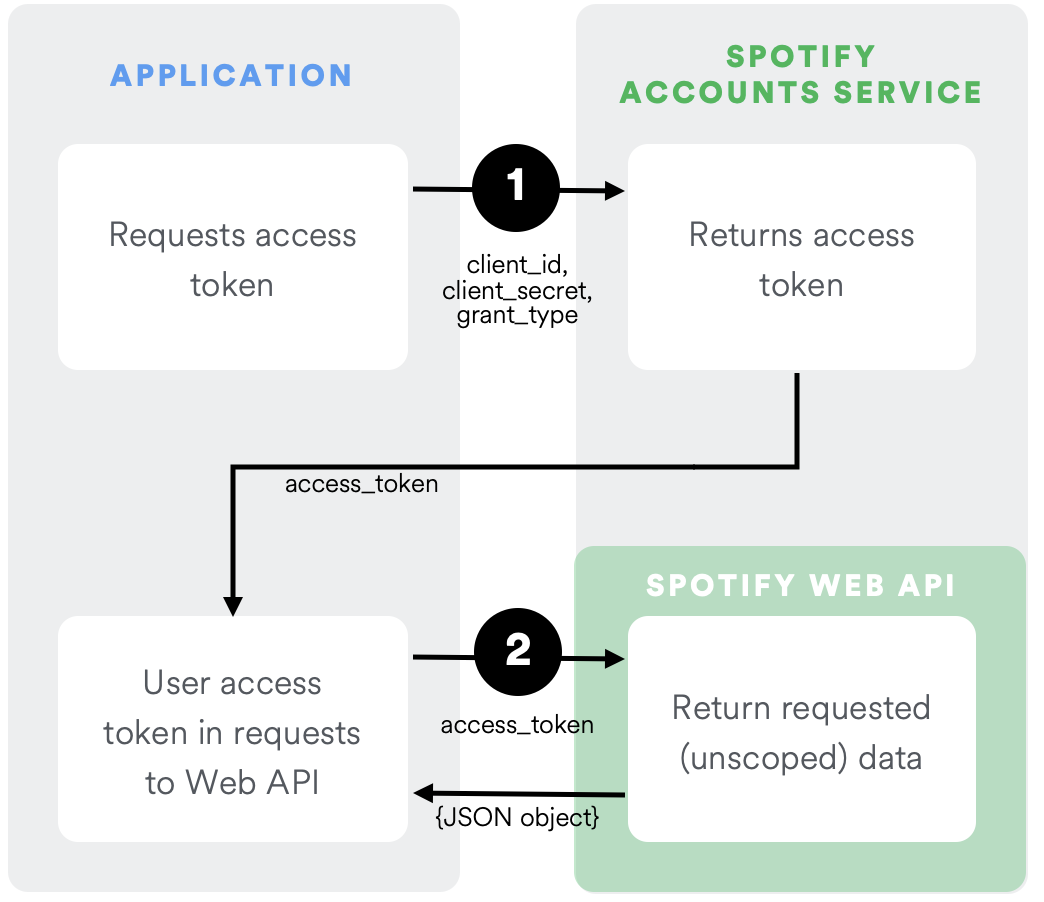
\includegraphics[width=0.6\textwidth]{SpotifyAuthFlow}
%    \\
%    Source: \cite{SpotifyAuth}
%\end{figure}
%
%Step one is a post request to the Spotify Account Service containing the client id and client secret in the body,
%which returns an access token valid for one hour.
%This token can be used to access any endpoint of the actual \ac{API} that does not require user specific data.
%When the token expires, a new one has to be requested before querying the \ac{API} again.
%Figure \ref{fig:Access Token Request} shows the full request and response to acquire the token.
%
%\begin{figure}[H]
%    \caption{Access Token Request}
%	\label{fig:Access Token Request}
%\begin{apiRoute}{post}{https://accounts.spotify.com/api/token}{request access token}
%    \begin{routeRequest}{application/x-www-form-urlencoded}
%        \begin{routeRequestBody}
%{
%    "grant_type": "client_credentials",
%    "client_id": client id from application dashboard,
%    "client_secret": client secret from dashboard
%}
%        \end{routeRequestBody}
%    \end{routeRequest}
%    \begin{routeResponse}{application/json}
%        \begin{routeResponseItem}{200}{ok}
%            \begin{routeResponseItemBody}
%{
%    "access_token": "BQDgQCSx-tIMDo9LfVeZxm6YMl2p_WbEU3Q9ENsVl7e--6d_vockTsfzMVUhPWiHSSnFUuHvm_9POA1kYEw",
%    "token_type": "Bearer",
%    "expires_in": 3600
%}
%            \end{routeResponseItemBody}
%        \end{routeResponseItem}
%    \end{routeResponse}
%\end{apiRoute}
%\end{figure}
%

\subsubsection{Getting Features}

In order to predict the genre of a track based on audio features, these features have to be requested
for every track. Spotify provides an endpoint to get audio features for up to 99 tracks at a time.
The typical request/response pattern for the audio-feature request endpoint is shown in figure \ref{fig:Audio Feature Request}.

\begin{figure}[H]
    \caption{Audio Feature Request}
	\label{fig:Audio Feature Request}
\begin{apiRoute}{get}{https://api.spotify.com/v1/audio-features?ids=\{ids\}}{request audio features for id}
    \methodJson
    \begin{routeParameter}
        \routeParamItem{ids}{comma seperated list of up to 99 song ids}
    \end{routeParameter}
    \begin{routeResponse}{application/json}
        \begin{routeResponseItem}{200}{ok}
            \begin{routeResponseItemBody}
{
    "audio_features": [
        {
            "danceability": 0.677,
            "energy": 0.638,
            "key": 8,
            "loudness": -8.631,
            "mode": 1,
            "speechiness": 0.333,
            "acousticness": 0.589,
            "instrumentalness": 0,
            "liveness": 0.193,
            "valence": 0.435,
            "tempo": 82.810,
            "type": "audio_features",
            "id": "2e3Ea0o24lReQFR4FA7yXH",
            "uri": "spotify:track:2e3Ea0o24lReQFR4FA7yXH",
            "track_href": "https://api.spotify.com/v1/tracks/2e3Ea0o24lReQFR4FA7yXH",
            "analysis_url": "https://api.spotify.com/v1/audio-analysis/2e3Ea0o24lReQFR4FA7yXH",
            "duration_ms": 211497,
            "time_signature": 4
        },
        ...
    ]
}
            \end{routeResponseItemBody}
        \end{routeResponseItem}
    \end{routeResponse}
\end{apiRoute}
\end{figure}

With the exception of \emph{type}, \emph{id}, \emph{uri}, \emph{track\_href} and \emph{analysis\_url}, all of the fields included in this response
can be used as features in the dataset. However, this api call expects a track id, which needs to be retrieved using
other api calls first. This could be a search endpoint, getting all tracks in a playlist, etc.
Also, it does not give the track or artist names and doesn't include a genre.

\subsubsection{Getting Track IDs and Labels}

There is no simple endpoint that takes one or more track ids and returns  a "genre" field
in its response. The exploration of the API revealed two ways of getting the genre of a track. 

The first way is using the artist of a track. Given a track id, the artists of the track and their corresponding
ids can be requested by using the \emph{/tracks/{id}} endpoint. Then, using the artist id, the genres that an
artist is known for are returned, as shown in figure \ref{fig:Artist Request}.

\begin{figure}[H]
    \caption{Artist Request}
	\label{fig:Artist Request}
\begin{apiRoute}{get}{https://api.spotify.com/v1/artists/\{id\}}{request information about an artist by their id}
    \begin{routeParameter}
        \routeParamItem{id}{id of the artist}
    \end{routeParameter}
    \begin{routeResponse}{application/json}
        \begin{routeResponseItem}{200}{ok}
            \begin{routeResponseItemBody}
{
    "external_urls": {
        "spotify": "link to resource.."
    },
    "followers": {
        "href": null,
        "total": 15554811
    },
    "genres": [
        "conscious hip hop",
        "hip hop",
        "north carolina hip hop",
        "rap"
    ],
    "href": "link to resource...",
    "id": "6l3HvQ5sa6mXTsMTB19rO5",
    "images": [ links to album covers... ],
    "name": "J. Cole",
    "popularity": 89,
    "type": "artist",
    "uri": "spotify:artist:6l3Hv..."
}
            \end{routeResponseItemBody}
        \end{routeResponseItem}
    \end{routeResponse}
\end{apiRoute}
\end{figure}

The examplary API response shows a problem with this approach. One artist can be sorted
into multiple genres.
A given track might be associated with either of the artist's genres, but the data does
not show, which one exactly.
Additionally a track might have multiple artists which further complicates this.
Given these circumstances, this approach is problematic.

The second way is Spotifys "categories" feature. The app's search tab provides a number of
categories that a user can browse to find new music in their preferred genre or style.
In figure \ref{fig:Categories and Playlists in Spotify App}a an overview over some of the categories
that are available in the Spotify app is shown. There are categories of multiple types like
places and activities, but also for all major genres. In the app screenshot
for example "Classical", "Jazz or "Soul".
These categories can be used to get tracks that belong in each specific category. When a user taps on
one of the categories, playlists that contain tracks of the respective category are shown to the user
(figure \ref{fig:Categories and Playlists in Spotify App}b).

\begin{figure}[H]
    \centering
    \subfloat[\centering Category Overview]{{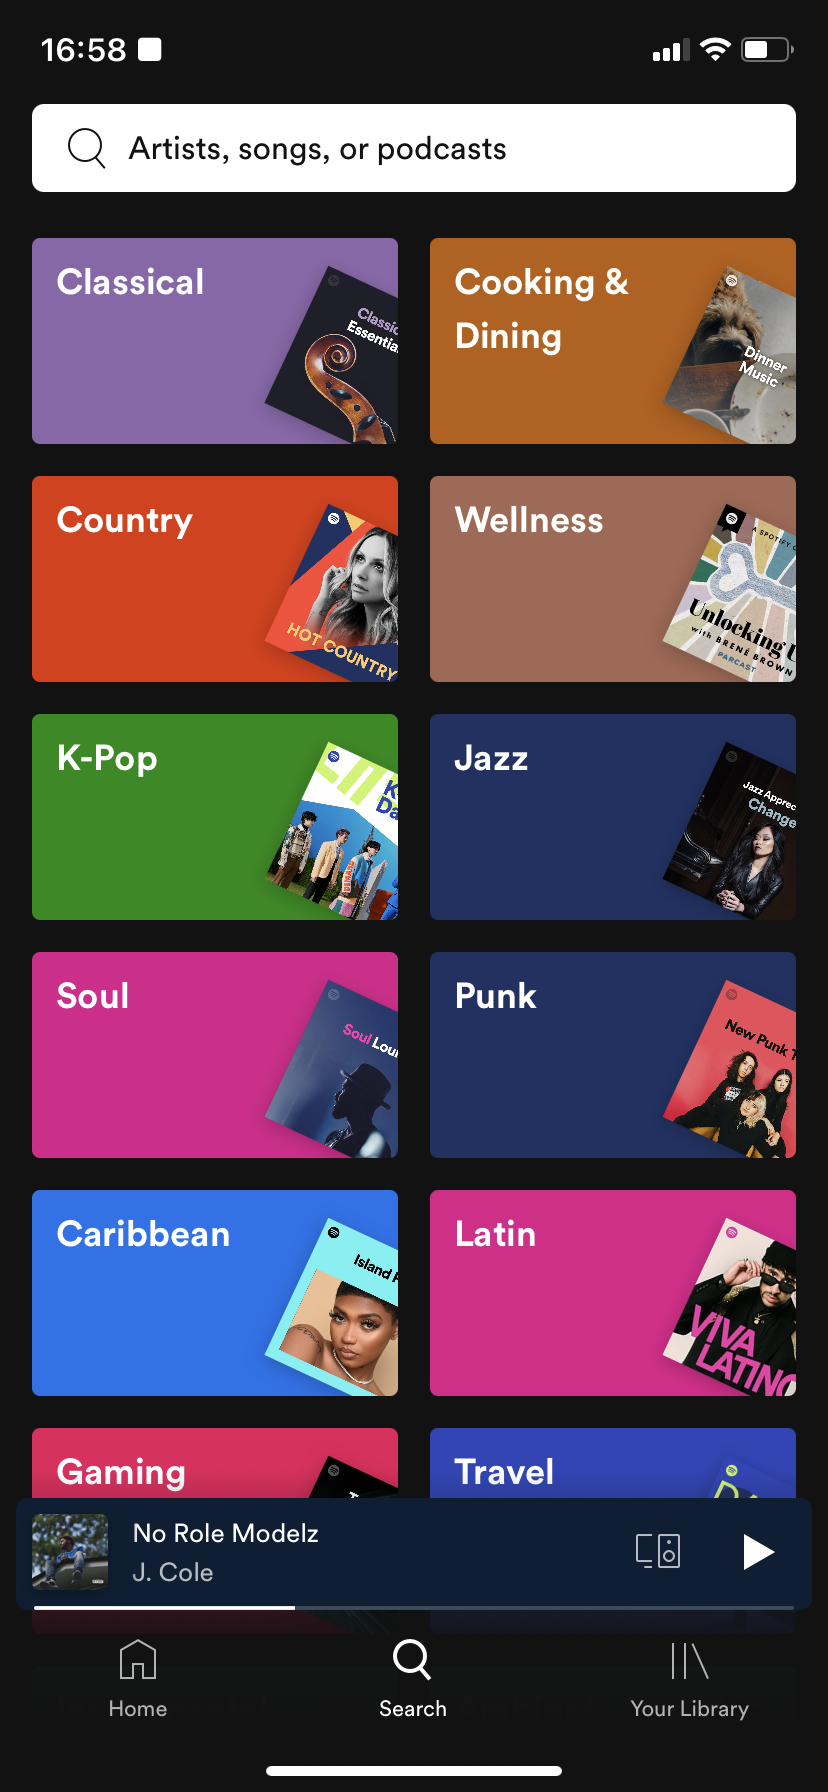
\includegraphics[width=4cm]{SpotifyCategoryOverview} }}%
    \qquad
    \subfloat[\centering Playlists in category]{{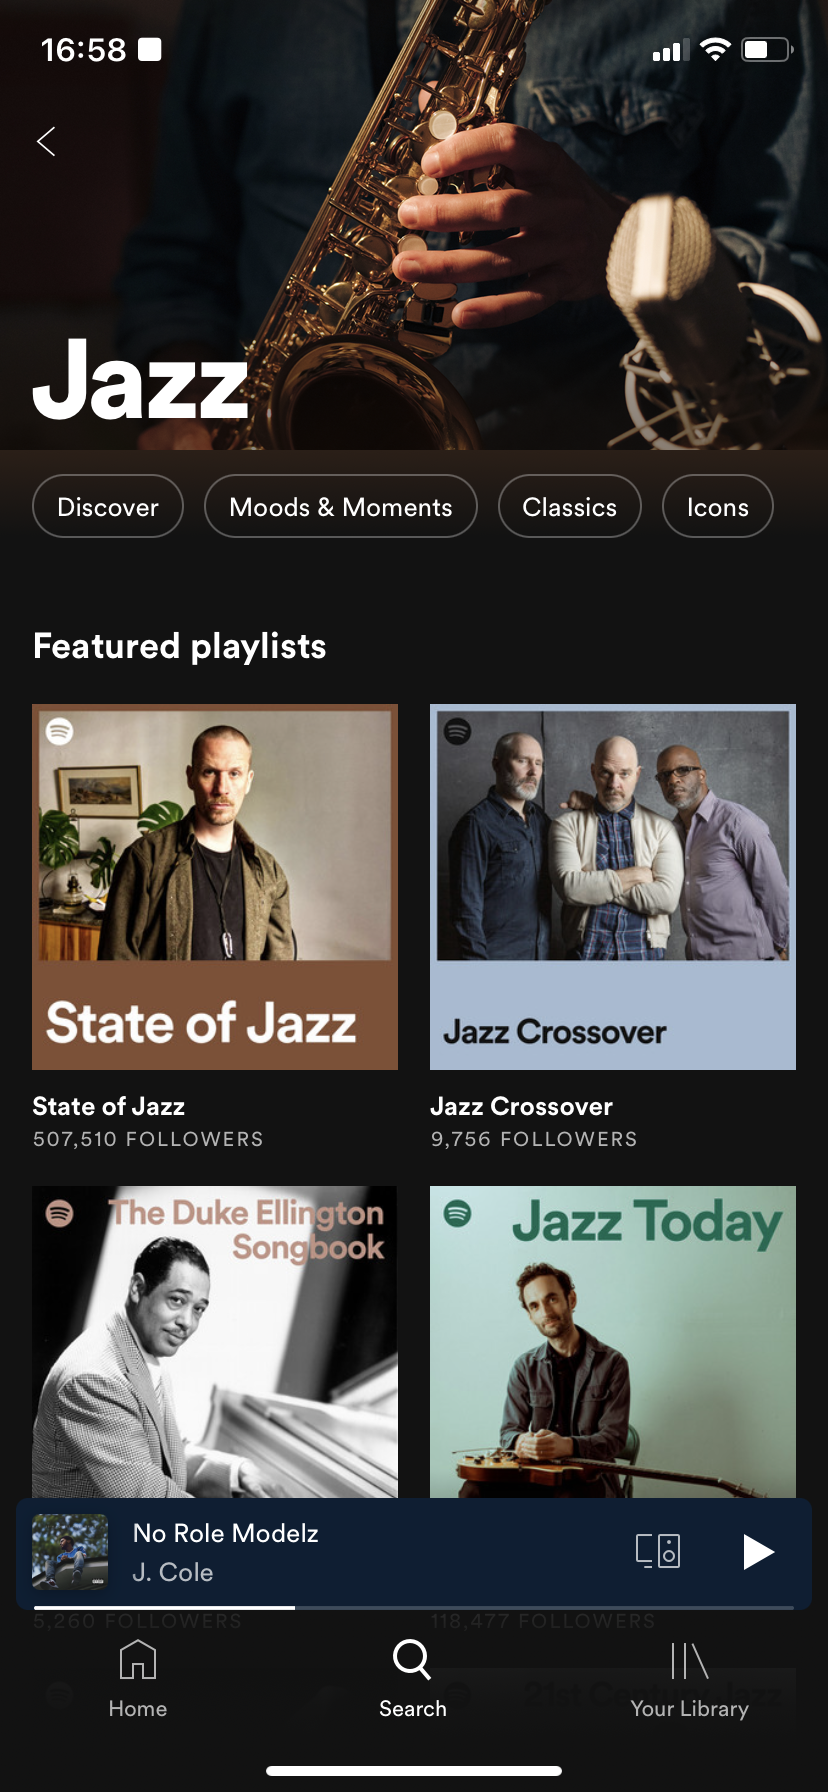
\includegraphics[width=4cm]{SpotifyPlaylistOverview} }}%
    \caption{Categories and Playlists in Spotify App}%
    \label{fig:Categories and Playlists in Spotify App}%
\end{figure}

The API mirrors the app's behaviour and provides an endpoint to get a list of categories and their ids,
one to get all playlists and playlist ids in a category, and one to get all tracks and track ids in
a playlist. This chain of API calls is used to request every track in every playlist in a certain category.


\subsubsection{Python Implementation}

This section describes, how the previously explained API calls are used to request data from the API
and save the complete dataset as a CSV file.
As explaining the Python code in detail is beyond the scope of this paper, only the general 
approach to the application is explained here. 
A well documented Jupyter Notebook containing all of the code is contained in the appendix and should be
refered to for further details (\ref{appendix}).

The script was implemented in a way that lets anyone with a Spotify
developer account run it to gather their own data.
It supports filtering for certain genres to speed up the process and exporting the current data after each step
to be able to pause the data collection and check the current results or continue later.
The details of these functions are explained in this section using code snippets.

The Python \emph{requests} library is used to execute the requests, as it supports the features needed to send the GET and POST
requests needed without having to write complicated code.
%The \emph{dotenv} library is used to read the credentials needed for authentication from a seperate .env file,
%rather than writing them into the code.
%This prevents sensitive credentials from being committed into version control, which is hosted in a public GitHub repository.
The \emph{json} library is used for transforming Python dictionaries into json data, \emph{math} for access to rounding functions,
\emph{os} for managing system paths and access to files, \emph{http} to define retry and timeout behaviour and \emph{csv}
to finally transform the json data into a CSV file.

After importing all necessary libraries, the credentials are read and a method is defined for authenticating to the API.
The http library is configured to minimize errors and exceptions due to late responses or failed requests.
A filter is implemented to limit the categories the data should be retrieved for using category ids.
Next, the four main steps of data collection are executed:

\begin{enumerate}
    \item Getting categories
    \item Getting playlists
    \item Getting tracks
    \item Getting audio features
\end{enumerate}

For each step, a method was implemented, which takes data from the previous step and uses it to request further data from the
API. Category ids are used to get a playlists category, playlist ids are used to get a playlists tracks and finally track ids
are used to request audio features.

After going through all stages of data retrieval, the following JSON datastructure has been built:

\begin{lstlisting}[language=Python]
{
  "categories": [
    {
      "id": "hiphop",
      "name": "Hip-Hop",
      "playlists": [
        {
          "id": "37i9dQZF1DX0XUsuxWHRQd",
          "name": "RapCaviar",
          "tracks": [
            {
              "id": "2AaJeBEq3WLcfFW1y8svDf",
              "name": "By Your Side",
              "album": {
                "id": "2RrZgDND03MLu6pRJdTkz5",
                "name": "By Your Side"
              },
              "artists": [
                {
                  "id": "45TgXXqMDdF8BkjA83OM7z",
                  "name": "Rod Wave"
                }
              ],
              "features": {
                "danceability": 0.649,
                "energy": 0.508,
                "key": 8,
                "loudness": -10.232,
                "mode": 1,
                "speechiness": 0.0959,
                "acousticness": 0.0345,
                "instrumentalness": 3.59e-05,
                "liveness": 0.0736,
                "valence": 0.405,
                "tempo": 157.975,
                "duration_ms": 194051,
                "time_signature": 4
              }
            },
            ...
\end{lstlisting}

This JSON contains all the necessary fields needed for continuing with the CRISP DM process.
To prepare the dataset for data analysis, the JSON data is transformed into a flat structure and stored in a CSV file.
The final structure of the data is shown in table \ref{tbl:Data after Import}.

\textbf{Tabelle hier einfügen}
%
%\begin{table}[H]
%    \centering
%\begin{tabular}{llllllllllrrrrrrrrrrrrr}
%\toprule
%categories.id & categories.name & categories.playlists.id & categories.playlists.name & categories.playlists.tracks.id & categories.playlists.tracks.name & categories.playlists.tracks.album.id & categories.playlists.tracks.album.name & categories.playlists.tracks.artists &  categories.playlists.tracks.features.danceability &  categories.playlists.tracks.features.energy &  categories.playlists.tracks.features.key &  categories.playlists.tracks.features.loudness &  categories.playlists.tracks.features.mode &  categories.playlists.tracks.features.speechiness &  categories.playlists.tracks.features.acousticness &  categories.playlists.tracks.features.instrumentalness &  categories.playlists.tracks.features.liveness &  categories.playlists.tracks.features.valence &  categories.playlists.tracks.features.tempo &  categories.playlists.tracks.features.duration\_ms &  categories.playlists.tracks.features.time\_signature 
%\midrule
%hiphop &         Hip-Hop &  37i9dQZF1DX0XUsuxWHRQd &                 RapCaviar &         2AaJeBEq3WLcfFW1y8svDf &                     By Your Side &               2RrZgDND03MLu6pRJdTkz5 &                           By Your Side &                            Rod Wave &                                              0.649 &                                        0.508 &                                         8 &                                        -10.232 &                                          1 &                                            0.0959 &                                            0.03450 &                                           0.000036 &                                         0.0736 &                                         0.405 &                                     157.975 &                                            194051 &                                                  4 \\\\\n1 &        hiphop &         Hip-Hop &  37i9dQZF1DX0XUsuxWHRQd &                 RapCaviar &         7uLFOXgLrS90tEYPO1DGXy &                Man in the Mirror &               1VxVQAgekwkFo8yoXvFZ8o &                                 B4 AVA &              A Boogie Wit da Hoodie &                                              0.849 &                                        0.631 &                                         3 &                                         -4.241 &                                          0 &                                            0.0637 &                                            0.17100 &                                           0.000000 &                                         0.1490 &                                         0.550 &                                     135.997 &                                            215304 &                                                  4 \\\\\n2 &        hiphop &         Hip-Hop &  37i9dQZF1DX0XUsuxWHRQd &                 RapCaviar &         2lUDBd7JrgAMltcp6dcd7D &                       25 million &               1eVrpJbHRLBbioB9sb5b94 &                         LIVE LIFE FAST &                         Roddy Ricch &                                              0.793 &                                        0.481 &                                         9 &                                         -9.258 &                                          1 &                                            0.1240 &                                            0.01900 &                                           0.000001 &                                         0.1390 &                                         0.395 &                                     132.202 &                                            204626 &                                                  4 \\\\\n3 &        hiphop &         Hip-Hop &  37i9dQZF1DX0XUsuxWHRQd &                 RapCaviar &         0qHPxjC83zQYcxe39xSShx &                         thailand &               1eVrpJbHRLBbioB9sb5b94 &                         LIVE LIFE FAST &                         Roddy Ricch &                                              0.875 &                                        0.478 &                                         7 &                                        -10.562 &                                          1 &                                            0.2180 &                                            0.00717 &                                           0.000000 &                                         0.1470 &                                         0.409 &                                     128.990 &                                            200959 &                                                  4 \\\\\n4 &        hiphop &         Hip-Hop &  37i9dQZF1DX0XUsuxWHRQd &                 RapCaviar &         2QIBJFl8DJR1mDh9GwfZef &       Don’t Play (with Lil Baby) &               2rLqUcipEjIKK9rma5OTN8 &                       Hall of Fame 2.0 &                     Polo G,Lil Baby &                                              0.684 &                                        0.624 &                                         2 &                                         -7.414 &                                          0 &                                            0.3470 &                                            0.23900 &                                           0.000000 &                                         0.1120 &                                         0.708 &                                     146.925 &                                            156735 &                                                  4 \\\\\n5 &        hiphop &         Hip-Hop &  37i9dQZF1DX0XUsuxWHRQd &                 RapCaviar &         1WGmhglF1ghRiHsx4YUq86 &                       Love \\& War &               720wVklJFHQgiLQuPpdCla &                             Love \\& War &                         Kodak Black &                                              0.762 &                                        0.649 &                                        11 &                                         -5.624 &                                          0 &                                            0.0527 &                                            0.58000 &                                           0.000017 &                                         0.0971 &                                         0.501 &                                     145.090 &                                            239146 &                                                  4 \\\\\n\\bottomrule\n\\end{tabular}
%\caption{Final Datastructure after collection}%
%\label{tbl:Data after Import}%
%\end{table} 


%First, the credentials are read using \emph{load\_dotenv}. Then a method is defined which takes the client id and secret as input,
%executes a POST request to the accounts API, as shown in \ref{fig:Access Token Request}, and return the access token from the
%\emph{access\_token} field in the response. 
%
%\begin{lstlisting}[language=Python]
%    #Get environment variables from ".env" file and read credentials
%    load_dotenv('.env')
%    client_id = os.environ.get('CLIENT_ID')
%    client_secret = os.environ.get('CLIENT_SECRET')
%   
%    # Authenticate and get an API Token from Spotify using a Client ID and secret
%    def getAuthTokenFromCredentials(id, secret):
%    
%        url = "https://accounts.spotify.com/api/token"
%    
%        payload = f'grant_type=client_credentials&client_id={id}&client_secret={secret}'
%        headers = {
%        'Content-Type': 'application/x-www-form-urlencoded',
%        }
%    
%        response = requests.request("POST", url, headers=headers, data=payload)
%    
%        return response.json()["access_token"]
%    
%    auth_token = getAuthTokenFromCredentials(client_id, client_secret)
%\end{lstlisting} 
%
%Next the http library is configured to use a ten second timeout and attempt five retries. If a request to the API is made
%and no response is given from Spotify's servers after ten seconds, the request will be sent again. If there is still no
%answer from the server after five attempts, an exception is thrown and the script ends.
%Timeouts are crucial as short disconnections from the Internet could result in the whole data collection step failing.
%The http setup code is found in appendix \ref{appendix:http setup}.
%
%The next part of the script implements the filter mechanism

%After importing all necessary libraries, the credentials are read and a method is defined for authenticating to the API.  Afterwards, the http library is configured to minimize errors and exceptions due to late responses or failed requests.  The code for these steps is shown in the appendix.  The next part of the script implements the filter mechanism: \begin{lstlisting}[language=Python] category_filter = None # comment this out if you don't want to set a filter category_filter = ["hiphop", "jazz", "rock"] # tells data collection functions to not use filter if it's not set if category_filter is not None: use_filter = True else: use_filter = False \end{lstlisting} This filter can be used to limit the categories that are to be taken into account when collecting the data.  Possible values are all valid category ids, which can be requested using the API call shown in figure \ref{fig:Categories Request}.  \begin{figure}[H] \caption{Categories Request} \label{fig:Categories Request} \begin{apiRoute}{get}{https://api.spotify.com/v1/categories?country=\{country\}\&locale=\{locale\}\&limit=\{limit\}\&offset=\{offset\}}{Get a list of categories used on Spotifys browse tab} \begin{routeParameter} \routeParamItem{id}{id of the artist} \routeParamItem{country}{only display categories available in a specific country} \routeParamItem{locale}{the language in which the categories should be returned} \routeParamItem{limit}{the maximum number of items to be returned} \routeParamItem{offset}{index of the first item to return} \end{routeParameter} \begin{routeResponse}{application/json} \begin{routeResponseItem}{200}{ok} \begin{routeResponseItemBody} { "categories": { "href": "...", "items": [ { ...  "id": "hiphop", "name": "Hip-Hop" }, { ...  "id": "pop", "name": "Pop" }, ...  ], ...  } } \end{routeResponseItemBody} \end{routeResponseItem} \end{routeResponse} \end{apiRoute} \end{figure} The response shows an \emph{id} field for each item in the items array.  These ids can be used in the filter list.  If the \emph{category\_filter} variable is undefined, no filter is set.  %Next, the option to import existing data from a file is given.  %If a user already has the json data containing all playlists for all categories they want to use, %they can load the json file here and skip executing the collection of categories and playlists and continue right %at the collection of tracks for each playlist.  % %\begin{lstlisting}[language=Python] %    data = {} % %    #To load data_object from file instead of rerunning the scripts, uncomment this: % %    file = open(os.path.join("data_collection", "json", "tracks_full.json")) %    data = json.load(file) %\end{lstlisting} 
%Next, the four main steps of data collection will be defined and executed:
%
%\begin{enumerate}
%    \item Getting categories
%    \item Getting playlists
%    \item Getting tracks
%    \item Getting audio features
%\end{enumerate}
%
%Each step is defined as a function with some input parameters and the resulting json data as output, which can then
%be used as input for the next step.
%
%The function definition for getting the categories looks like this:
%
%\begin{lstlisting}[language=Python]
%    def getAllCategories(
%        # takes the requests session, which was set up in the beginning
%        requests_session,
%        # this is the token which was retrieved in the authorization step
%        auth_token,
%        # set to True if the category_filter should be used
%        use_category_filter=False, 
%        # this takes the list which is used as a category filter
%        category_filter=None,  
%        # set to True if the result of this step should be written into a json file
%        write_to_file=False, 
%        # give the file path at which the json file should be stored
%        path_to_file=''): 
%\end{lstlisting}
%
%The function first makes a simple API call with \emph{limit=1} to get the total amount of categories available.
%This is necessary, because the API returns a maximum number of 50 entries per request, so if the total number of
%items exceeds 50, multiple calls have to be made.
%
%\begin{lstlisting}[language=Python]
%    # Establishing the requests session
%    http = requests_session
%
%    # First API call used to get the total amount of categories
%    headers = { 'Authorization': f'Bearer {auth_token}' }
%    url = "https://api.spotify.com/v1/browse/categories?country=US&locale=en_US&limit=1"
%    
%    try:
%        response = http.request("GET", url, headers=headers, data={})
%        if response.status_code != requests.codes.ok:
%            raise Exception
%    except Exception as e:
%        raise SystemExit(e)
%\end{lstlisting}
%
%\emph{headers} contains the HTTP headers needed for authentication.
%The URL is given with the right country and locale settings and the request is sent inside of a try block.
%If the response doesn't contain an HTTP status code 200, an Exception is raised and the program is stopped,
%as there is possibly an error in the request or response which could mean corrupted data.
%
%Next, the total amount of categories is extracted from the response and the number of pages is calculated.
%
%\begin{lstlisting}[language=Python]
%    categoryAmount = response.json()["categories"]["total"]
%
%    # API only returns 50 items at a time. Offset can be used to gradually get all items
%    # Calculate number of pages with 50 items
%    pages = int(math.ceil(categoryAmount/50))
%    data = {"categories": []}
%\end{lstlisting}
%
%By dividing the category amount by 50 and rounding up to the next integer, the number of API calls necessary to get 
%all entries is calculated. Each call returns a "page" of items, page one contains items 0 to 49 and is retrieved by
%using offset 0 and limit 50, page two contains items 50 to 99 and is retrieved by using offset 50 and limit 50,
%and so on.
%
%A for loop is used to execute the request for every page as shown before.
%Each category's id and name are read from the response and appended to the data object:
%
%\begin{lstlisting}[language=Python]
%    for x in range(pages):
%        url = f"https://api.spotify.com/v1/browse/categories?country=US&locale=en_US&limit=50&offset={x * 50}"
%        
%        try:
%            response = http.request("GET", url, headers=headers, data={})
%            if response.status_code != requests.codes.ok:
%                raise Exception
%        except Exception as e:
%            raise SystemExit(e)
%        
%        # categories are stored in the data dictionary
%        for el in response.json()["categories"]["items"]:
%            if (use_category_filter == True and el["id"] in category_filter) or use_category_filter == False:
%                data["categories"].append({
%                    "id": el["id"], 
%                    "name": el["name"]
%                })
%\end{lstlisting}
%
%Outside of the for loop, the resulting data is written to a file if \emph{write\_to\_file} was set to \emph{True} and the 
%data object is returned:
%
%
%\begin{lstlisting}[language=Python]
%    if write_to_file == True:
%        with open(path_to_file, 'w') as outfile:
%            json.dump(data, outfile, indent=2)
%
%    return data
%\end{lstlisting}

%The data collected after this step looks like this:
%
%\begin{lstlisting}[language=Python]
%{
%    "categories": [
%        {
%            "id": "hiphop",
%            "name": "Hip-Hop"
%        },
%        {
%            "id": "pop",
%            "name": "Pop"
%        },
%        ...
%    ]
%}
%\end{lstlisting}
%
%This concludes the function \emph{getAllCategories}.
%The data retrieved from this step is used for the next step, getting the playlists.
%The function definition here is slightly different:
%
%\begin{lstlisting}[language=Python]
%    def getPlaylistsForCategories(
%        requests_session,
%        auth_token,
%        data_object,
%        write_to_file=False,
%        path_to_file=''):
%\end{lstlisting}
%
%Instead of the filtering options, which only apply to the categories, this function takes the \emph{data\_object} from the
%previous step. This could be passed in directly from the previous function or read from a file.
%The function implements a nested for loop. The outer loop iterates over all categories in the data object.
%The inner loop uses an endpoint to get each category's playlists.
%The API request/response is shown in figure \ref{fig:Get Category's Playlists Request and Response}.
%
%\begin{figure}[H]
%    \caption{Get Category's Playlists Request and Response}
%	\label{fig:Get Category's Playlists Request and Response}
%\begin{apiRoute}{get}{https://api.spotify.com/v1/categories/\{category\_id\}/playlists?country=\{country\}\&limit=\{limit\}\&offset=\{offset\}}{Get Category's Playlists}
%    \begin{routeParameter}
%        \routeParamItem{category\_id}{category id}
%        \routeParamItem{country}{only display categories available in a specific country}
%        \routeParamItem{limit}{the maximum number of items to be returned}
%        \routeParamItem{offset}{index of the first item to return}
%    \end{routeParameter}
%    \begin{routeResponse}{application/json}
%        \begin{routeResponseItem}{200}{ok}
%            \begin{routeResponseItemBody}
%{
%  "playlists": {
%    "href": "...",
%    "items": [
%      {
%        "collaborative": false,
%        "description": "New music from YoungBoy...",
%        "external_urls": ...
%        "href": "...",
%        "id": "37i9dQZF1DX0XUsuxWHRQd",
%        "images": ...
%        "name": "RapCaviar",
%        "owner": ...
%        "primary_color": null,
%        "public": null,
%        "snapshot_id": "...",
%        "tracks": {
%          "href": "...",
%          "total": 50
%        },
%        "type": "playlist",
%        "uri": "spotify:playlist:37i9dQZF1DX..."
%      },
%      ...
%    ],
%    "limit": 50,
%    "next": "...",
%    "offset": 0,
%    "previous": null,
%    "total": 50
%  }
%}
%            \end{routeResponseItemBody}
%        \end{routeResponseItem}
%    \end{routeResponse}
%\end{apiRoute}
%\end{figure}

%As there is an upper limit of 50 playlists per request, the same paging method is used as in the category function.
%If an item's \emph{type} is not \emph{playlist}, it is filtered out, as it doesn't fit the schema.
%Each playlists name and id is stored in the data object, which is returned from the function.
%The JSON data after this step looks like this:
%
%\begin{lstlisting}[language=Python]
%{
%    "categories": [
%        {
%        "id": "hiphop",
%        "name": "Hip-Hop",
%        "playlists": [
%            {
%            "id": "37i9dQZF1DX0XUsuxWHRQd",
%            "name": "RapCaviar"
%            },
%            {
%            "id": "37i9dQZF1DX6GwdWRQMQpq",
%            "name": "Feelin' Myself"
%            },
%            ...
%        },
%        ...
%    }
%}
%\end{lstlisting}
%
%The third step gets all tracks in each playlist. The function definition is the same as before, as this function also
%takes data from the previous step. This time, there are three nested for loops. One for looping through the categories,
%then another one for looping through the playlists. In this one the number of pages is calculated.
%The third loop requests the pages and appends the tracks to the playlist data.
%The request parameters for this request differ from the other steps.
%There is a market parameter, which essentially functions equally to country.
%There is also a fields parameter, which takes a string that can be used to define which fields the API should
%return. This is done to save bandwith, as the response of this endpoint is very large and most
%of the datapoints might not be needed by the client.
%In this case, the value \emph{items(track(name, id, album(name, id), artists)), total} is used to return only
%items of type track, their id and name, their albums name and id, and their artist information.
%Also the total amount of tracks in the playlist is returned.
%The parameter \emph{additional\_types} is set to \emph{track}, as podcasts are irrelevant to this analysis.
%An examplary API request/response is shown in figure \ref{fig:Get Playlist's Tracks}.
%Because a track can have multiple artists, each artist's name and id are extracted and saved with the track.
%The function code can be found in the appendix.
%
%\begin{figure}[H]
%    \caption{Get Playlist's Tracks}
%	\label{fig:Get Playlist's Tracks}
%\begin{apiRoute}{get}{https://api.spotify.com/v1/playlists/\{playlist\_id\}/tracks?market=\{market\}\&fields=\{fields\}\&additional\_types=\{additional\_types\}\&limit=\{limit\}\&offset=\{offset\}}{Get Playlist's Tracks}
%    \begin{routeParameter}
%        \routeParamItem{playlist\_id}{playlist id}
%        \routeParamItem{market}{only display items available in this market}
%        \routeParamItem{fields}{a string describing which fields to return}
%        \routeParamItem{additional\_types}{supported item types. valid types are "track" and "episode"}
%        \routeParamItem{limit}{the maximum number of items to be returned}
%        \routeParamItem{offset}{index of the first item to return}
%    \end{routeParameter}
%    \begin{routeResponse}{application/json}
%        \begin{routeResponseItem}{200}{ok}
%            \begin{routeResponseItemBody}
%{
%  "items": [
%    {
%      "track": {
%        "album": {
%          "id": "4oxmme6i4mypSt2DDzPTsW",
%          "name": "DS4EVER"
%        },
%        "artists": [
%          {
%            "external_urls": {
%                "spotify": "..."
%            },
%            "href": "...",
%            "id": "2hlmm7s2ICUX0LVIhVFlZQ",
%            "name": "Gunna",
%            "type": "artist",
%            "uri": "spotify:artist:2hlmm7s2ICUX0LVIhVFlZQ"
%          },
%          ...
%        ]
%      }
%    },
%    ...
%  ],
%  "total": 50
%}
%            \end{routeResponseItemBody}
%        \end{routeResponseItem}
%    \end{routeResponse}
%\end{apiRoute}
%\end{figure}
%
%The fourth step is getting the audio features for each track.
%The request that is used was already shown in \ref{fig:Audio Feature Request}
%The function used has the same definition as before but implements one more for loop to iterate through
%the tracks. Again, the code for this step is found in the appendix.
%
%The data collected after this step looks like this:
%
%\begin{lstlisting}[language=Python]
%{
%  "categories": [
%    {
%      "id": "hiphop",
%      "name": "Hip-Hop",
%      "playlists": [
%        {
%          "id": "37i9dQZF1DX0XUsuxWHRQd",
%          "name": "RapCaviar",
%          "tracks": [
%            {
%              "id": "2AaJeBEq3WLcfFW1y8svDf",
%              "name": "By Your Side",
%              "album": {
%                "id": "2RrZgDND03MLu6pRJdTkz5",
%                "name": "By Your Side"
%              },
%              "artists": [
%                {
%                  "id": "45TgXXqMDdF8BkjA83OM7z",
%                  "name": "Rod Wave"
%                }
%              ],
%              "features": {
%                "danceability": 0.649,
%                "energy": 0.508,
%                "key": 8,
%                "loudness": -10.232,
%                "mode": 1,
%                "speechiness": 0.0959,
%                "acousticness": 0.0345,
%                "instrumentalness": 3.59e-05,
%                "liveness": 0.0736,
%                "valence": 0.405,
%                "tempo": 157.975,
%                "duration_ms": 194051,
%                "time_signature": 4
%              }
%            },
%            ...
%\end{lstlisting}
%
%This JSON contains all the necessary fields needed for continuing with the CRISP DM process.
%To prepare the dataset for data analysis, the JSON data needs to be transformed into a flat structure to
%be stored as a CSV file.
%Another Python function is used to flatten the data. It takes the resulting data from the last step and
%transforms it into the following format.
%
%\begin{lstlisting}[language=Python]
%[
%    {
%        "categories.id": "hiphop",
%        "categories.name": "Hip-Hop",
%        "categories.playlists.id": "37i9dQZF1DX0XUsuxWHRQd",
%        "categories.playlists.name": "RapCaviar",
%        "categories.playlists.tracks.id": "2AaJeBEq3WLcfFW1y8svDf",
%        "categories.playlists.tracks.name": "By Your Side",
%        "categories.playlists.tracks.album.id": "2RrZgDND03MLu6pRJdTkz5",
%        "categories.playlists.tracks.album.name": "By Your Side",
%        "categories.playlists.tracks.artists": "Rod Wave",
%        "categories.playlists.tracks.features.danceability": "0.649",
%        "categories.playlists.tracks.features.energy": "0.508",
%        "categories.playlists.tracks.features.key": "8",
%        "categories.playlists.tracks.features.loudness": "-10.232",
%        "categories.playlists.tracks.features.mode": "1",
%        "categories.playlists.tracks.features.speechiness": "0.0959",
%        "categories.playlists.tracks.features.acousticness": "0.0345",
%        "categories.playlists.tracks.features.instrumentalness": "3.59e-05",
%        "categories.playlists.tracks.features.liveness": "0.0736",
%        "categories.playlists.tracks.features.valence": "0.405",
%        "categories.playlists.tracks.features.tempo": "157.975",
%        "categories.playlists.tracks.features.duration_ms": "194051",
%        "categories.playlists.tracks.features.time_signature": "4"
%    }, 
%    ...
%]
%\end{lstlisting}
%
%The function is also found in the appendix.
%Notice, that the nested fields and arrays have been flattened to represent a two dimensional data structure
%containing only one array to represent rows which contains JSON objects with 22 fields. Each field represents
%a column. In the original JSON data, \emph{artists} is a list containing one or more entries.
%If the data was flattened in a way that groups the entries by each individual artist,
%there could be multiple rows for the same track.
%If for example \emph{track1} had two artists \emph{artist1} and \emph{artist2}, there would be two datapoints,
%both containing the same song name, id and features, but different artists.
%As the dataset should be grouped by individual tracks, not by artists,
%multiple artists are condensed into a comma-seperated list during flattening.
%This list is stored in the \emph{categories.playlists.tracks.artists} field.
%This means, that the individual artist data is lost in favor of grouping the dataset by tracks.
%
%After this process, the resulting two-dimensional structure is converted to a CSV file and saved for
%further processing.
\subsection{Data Understanding}

\subsubsection{Spotify}
Spotify is a music streaming service and has established itself as the Number one in this market. 
Since their launch in 2006, the company has gained over \(365\) million users, of which nearly \(45\) percent
are subscribed to the chargeable premium service. 
This Premium service comes at a subscription cost of nowadays \(12,99\)€ per month,
giving the opportunity to listen to every song that is available at Spotify - this being
ca. \(70\) million tracks from over \(1,2\) million Artists.

Similar to other streaming services, Spotify also generates a lot of data.
The question here is how to filter out data from music in order to personalize user accounts. 
The founders evaluated millions of songs and taught an AI to independently recognize
patterns and certain structures within different genres. 
The results of the algorithm can be seen above all in the "Discovery Weekly Playlist". 
Users are presented with thirty songs that match their tastes here every Monday.
At the moment, the Spotify algorithm, which to this day goes by the name Echo Nest,
works because of three main components. 

First of all, it creates an individual Taste Profile for each Spotify user. 
There, it is recorded which artists, songs, albums, playlists and also podcast and audio books the
respective user listens to. 
And also how long he listens to the music tracks, where he does it and how often.
This data is then compared with the Taste Profiles of other users. 
For example, if another user has a large overlap in musical taste with your own playlists,
you will be shown songs in the Discovery Weekly playlist that the other user already listens to regularly.
Playlists with more followers end up in the Discovery Weekly folders more often than those with
fewer followers. 

In addition, the algorithm analyzes the individual components of the music tracks. 
It breaks down each song available on Spotify by tempo, instruments, duration, highs and lows,
timbre, and so on. 
Based on the large amount of data, the Spotify algorithm divides the songs into more than 1500
different genres so far. 
However, in addition to many regional differences in music genres, "nonsensical" genres keep
coming out in the AI's analysis. While it might be able to imagine something under deep power pop punk,
genres like djent are not really close to reality. 

This analysis step also includes the classification of songs into happy, sad,
melancholic or other types of music, so the classification according to feelings.
However, this feature is also controversial among experts, because there is no actual definition of sad or happy music. 
That always depends on the individual listener and his mood. To support the AI at this point,
it reads the titles of the playlists of the users. 
If a song often lands in playlists with titles like love songs or romantic music,
the AI assumes that the song is to be rated as a love song. 

At last, the Echo Nest algorithm searches the entire web daily for blog posts, comments on websites,
articles, YouTube videos, Facebook postings and comments and tweets, 
evaluates them, and uses them to create an opinion about a particular song.
Thus, within a few days, the algorithm notices how a song is received overall.  
This quickly creates a specific rating for each track, which in turn influences the
Discover function and other recommendation formats within the platform. 

\subsubsection{Feature analysis}
In the course of the analysis carried out here, three different genres were selected in order
to subsequently assign songs to the correct genre on the basis of the underlying data. 
The genres selected here are \emph{\emph{rock}}, \emph{\emph{hiphop}} and \emph{\emph{jazz}}. The selection was made under the original, 
subjective assumption that these genres differ particularly strongly in their characteristics and style. 
The assumption focused primarily on characteristics such as vocals, the general use of instruments,
the instruments used, or the energy of the songs of the respective genre.

The important insight for further consideration of the analysis is here:
Each genre that is considered, each song feature that is evaluated does not reflect reality, 
but only reflects the results of the Spotify algorithm. The analysis can,
according to subjective opinion, assign a \emph{\emph{hiphop}} song to the category, 
or the genre \emph{rock} without being wrong - since the assignment makes sense based on the Spotify evaluations. 
Since the categories in the selected genres are very accurate due to their popularity,
the analysis is performed under the assumption that the two are congruent. 

As already mentioned, every song has given thirteen Features, which break down his main attributes into numbers.
To understand the data, it is crucial to get to know these features.
For a better presentation, they are divided into four clusters below, 
Musical Standards, Mood, Properties and Context.

\textbf{Musical Standards}

This Cluster includes the features, that capture and reflect the standard properties of music. 
These features are \emph{duration}, \emph{key}, \emph{mode} and \emph{time signature}. 
The feature \emph{duration}, as the name suggests, holds the information of how long the Track is.
This is measured in seconds. The feature \emph{key} is measured with an Integer between \(-1\) and \(11\) and 
holds information about the key the track is in. Integers map to pitches using standard Pitch Class notation, E.g., \(0\) = C, \(1\) = C\(\sharp\) /D\(\flat\), \(2\) = D, and so on. 
If no key was detected, the value is \(-1\).
\emph{mode} is an integer (either \(0\) or \(1\)) and indicates the modality (major or minor) of a track. Major is represented by \(1\) and minor is \(0\). 
At last, the feature \emph{time signature} is measured in an integer between \(3\) and \(7\).
It is a notational convention to specify how many beats are in each bar (or measure). 
The time signature ranges from \(3\) to \(7\) indicating time signatures of "3/4", to "7/4".

\textbf{Mood}

Following these features comes the cluster "Mood".
This cluster lists those features that measure the emotive values in songs, 
i.e. whether the song encourages dancing, spreads a positive or rather negative mood,
etc. This is captured with the features: \emph{danceability}, \emph{valence}, \emph{energy} and \emph{tempo}.

All of these features except \emph{tempo} are measured in a float between \(0\) and \(1\). 
\emph{danceability} describes how suitable a track is for dancing based on a combination of musical elements
including tempo, rhythm stability, beat strength, and overall regularity. A value of \(0.0\) is least danceable and 1.0 is most danceable.
\emph{valence} describes the musical positiveness conveyed by a track. 
Tracks with high valence sound more positive (e.g. happy, cheerful, euphoric),
while tracks with low valence sound more negative (e.g. sad, depressed, angry).  
\emph{energy} represents a perceptual measure of intensity and activity. Typically, energetic tracks feel fast, loud, and noisy. 
A value near \(1.0\) indicates high energy, while tracks near \(0.0\) indicates low Values in this Feature. 
At last, \emph{tempo} holds the information about the overall estimated tempo of a track in beats per
minute (BPM). In musical terminology, tempo is the speed or pace of a given piece and derives directly from the
average beat duration.

\textbf{Properties}

This next cluster includes all features that capture the audio characteristics of the tracks,
such as \emph{loudness}, \emph{speechiness} and \emph{instrumentalness}.

\emph{loudness} is measured in a float number between \(-60\) and \(0\) and measures the overall loudness
of a track in decibels (dB). 
The values are averaged across the entire track and are useful for comparing relative
loudness of tracks. 
\emph{speechiness}, measured in a float number between \(0\) and \(1\), detects the presence of spoken words in a track. 
The more exclusively speech-like the recording (e.g. talk show, audio book, poetry),
the closer to \(1.0\) the attribute value. 
Values above \(0.66\) describe tracks that are probably made entirely of spoken words. Values below \(0.33\) most likely represent music and other non-speech-like tracks. 
\emph{instrumentalness}, measured in a float between \(0\) and \(1\) as well, plays the counterpart to \emph{speechiness}.
It predicts whether a track contains no vocals at all. "Ooh" and "aah" sounds are treated as instrumental in this context.
The closer the \emph{instrumentalness} value is to \(1.0\), the more likely the track contains no vocal content. 
Values above \(0.5\) are intended to represent instrumental tracks, but confidence is higher as the value approaches \(1.0\).

\textbf{Context}

At last, this Cluster unions the Features \emph{liveness} and \emph{accousticness}.
These capture everything around the Songs, for example if it is played in front of a live audience.

Both Features are measured in a float number between \(0\) and \(1\).
\emph{accousticness} is a confidence measure from \(0.0\) to \(1.0\) of whether the track is acoustic. \(1.0\) represents high confidence the track is acoustic. 
\emph{liveness} detects the presence of an audience in the recording. 
Higher \emph{liveness} values represent an increased probability that the track was performed live.
A value above \(0.8\) provides strong likelihood that the track is live. 

\subsubsection{Overall correlation}
After these explanations, the characteristics of the features in the individual categories are evaluated.
A correlation matrix is used for this purpose. This shows on a scale between \(1\) and \(-1\) how
features correlate with each other. Since every song uses every feature,
a high correlation here does not mean that the features often appear together,
but how similar the values per song are. To start with an overall look over the data,
fig. \ref{fig:du_cm_overall}  shows a genre independent matrix.
This means that the features of all songs that could be gathered in the step of data
collection were analyzed to create this figure. 

\begin{figure}[H]
    \centering
    \caption[]{Correlation matrix: categorie-independent correlation of features}
	\label{fig:du_cm_overall}
    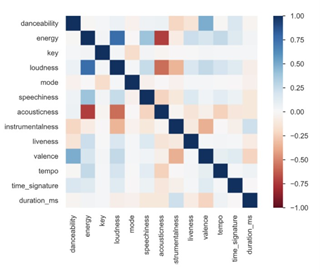
\includegraphics[width=0.4\textwidth]{output_overall.png}
\end{figure}

Generally, the features of the "Musical Standards" cluster can be ignored in this representation,
as they do not measure but only reflect characteristics (e.g., time signature or key).
It can be seen that \emph{energy} and \emph{loudness} have the highest correlation of the features,
with a value of approx. \(0.65\).  
%So, energetic songs often seem to be loud as well.
%This can be easily explained, since, as explained in the definition of the features:
%"Typically, energetic tracks feel fast, loud, and noisy".
In addition, there is a comparatively high correlation between \emph{valence} and "Dancebility" of
about \(0.5\). 
%which means that positive songs, i.e., songs with a high value for Valence,
%encourage more dancing than rather negative ones. 
The correlation between \emph{energy} and "\emph{accousticness}" is particularly negative, with a value of approx. \(-0.7\).
%Acoustic tracks therefore often do not seem to be very energetic and vice versa.
The same can be said for \emph{accousticness} and \emph{loudness}, with a correlation value of about \(-0.5\).
Outside of these extreme values, the remaining correlation values settle between \(-0.2\) and \(0.2\).
Worth mentioning here are the correlations between \emph{instrumentalness} and \emph{loudness} at
approx. \(-0.3\) as well as \emph{instrumentalness} and Valence also at approx. \(-0.3\). Furthermore,
in the positive \emph{speechiness} and \emph{energy} at a value of approx. \(0.3\).

\begin{figure}[H]
    \centering
    \subfloat[\centering Correlation matrix: categorie \emph{rock}]{{\includegraphics[width=4cm]{output_\emph{rock}.png} }}%
    \qquad
    \subfloat[\centering Correlation matrix: categorie \emph{hiphop}]{{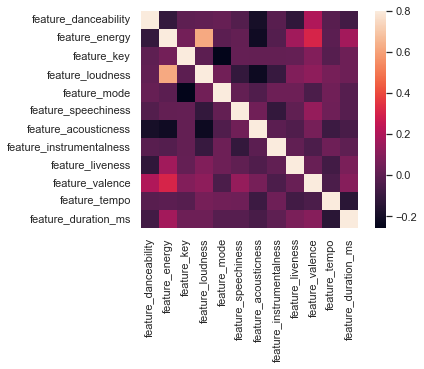
\includegraphics[width=4cm]{output_Hip_Hop.png} }}%
    \qquad
    \subfloat[\centering Correlation matrix: categorie \emph{jazz}]{{\includegraphics[width=4cm]{output_\emph{jazz}.png} }}%
    \caption{Correlations inside categories}%
    \label{fig:du_cm_categorie_dependent}%
\end{figure}

These correlations above now show the matrix on a category-specific basis.
It can be seen that the patterns described above also appear there.
However, the average correlation changes depending on the category.
For example, \emph{\emph{hiphop}} has the same characteristics as the independent matrix category but shows
fundamentally more negative correlations (cf. Fig. \ref{fig:du_cm_categorie_dependent}).

\subsubsection{Correlation Music theorie - Data}
In the final step of Data Understanding,
the music theory described in the basic section is compared to the data used in the analysis.
This is necessary to develop a deeper understanding of the data.
As mentioned at the beginning of this chapter, theory and Spotify are not always necessarily congruent,
which is why a clear delineation is important here.
For this purpose, the properties of the genres in the music theory are tried to be compared
with the help of the features (e.g., "You can't dance well to \emph{rock}" - What is the overall value for Danceability?).
To do this comparison, three features are chosen and discussed more deeply.
Subsequently, a better picture can be obtained with the help of further representations.

Starting with \emph{\emph{rock}}, one feature can be extracted here: The songs are mostly loud.
\emph{loudness} captures this property very well.
It measures the actual, average loudness of a song in decibels, with most tracks falling
in the \(-60\) to \(0\) range, where \(-60\) is very quiet and \(0\) is very high.
Overall, across all three categories, this feature has an average of -8.2544,
with a minimum value of \(-32.06\) and a maximum value of \(2.044\).

\begin{figure}[H]
    \centering
    \subfloat[\centering Distribution plot: \emph{loudness}]{{\includegraphics[width=4cm]{output_loudness.png} }}%
    \qquad
    \subfloat[\centering Boxplot: \emph{loudness}]{{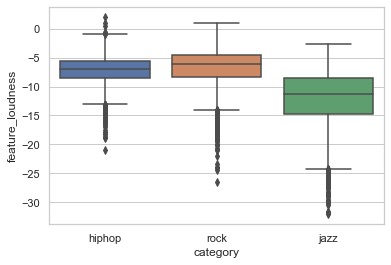
\includegraphics[width=4cm]{output_Loudness_boxplot.png} }}%
    \caption{\emph{loudness} compared in the different categories}%
    \label{fig:du_dp_bp_ln_categorie_dependent}%
\end{figure}

Figure \ref{fig:du_dp_bp_ln_categorie_dependent} shows a so-called distribution plot.
The X-axis contains the scale of the feature used (in this case \emph{loudness}).
The Y-axis reflects the density of the respective category, meaning the more songs are found in the respective value, the higher the density.
As can be seen in the figure, all categories offer a very wide range of volume levels.
\emph{jazz} spreads its songs over an area from \(-32.06\) (smallest value overall) to \(-2.695\) but locates
most songs at about \(-10\). \emph{\emph{hiphop}} and \emph{rock} go less wide but can accommodate more songs in the upper
quarter of the scale. \emph{rock} places its point furthest to the right of the scale.
Thus, it can be confirmed that \emph{rock} can generally be classified as loud,
but also shows as the loudest of the three categories.
However, it must also be emphasized here that \emph{\emph{hiphop}} comes shortly after.
In addition, \emph{jazz} is not as loud as the other two categories, but it serves a much wider range. 

The next feature that can be scrutinized here is the large occurrence of instruments in \emph{jazz}.
This can be checked in the Spotify data via the \emph{instrumentalness} feature.
It measures the sole presence of instruments in songs with values between \(0\) and \(1\).
The closer the value approaches \(1\), the higher the probability that there are no vocals or other
elements in the song. The overall average for this feature is \(0.174\).
The lowest value overall is \(0.0\) while the highest goes up to \(0.989\).

\begin{figure}[H]
    \centering
    \subfloat[\centering Distribution plot: \emph{instrumentalness}]{{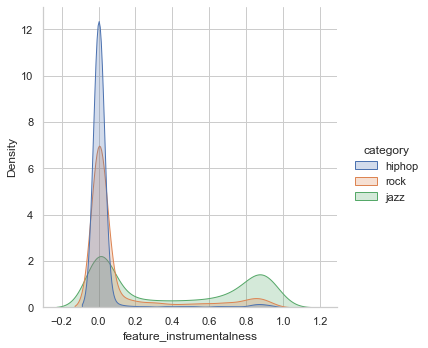
\includegraphics[width=4cm]{output_instumentelness.png} }}%
    \qquad
    \subfloat[\centering Boxplot: \emph{instrumentalness}]{{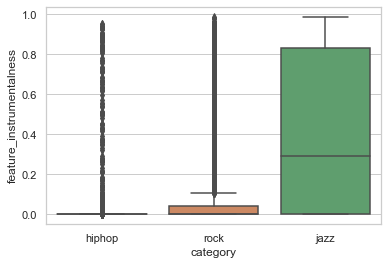
\includegraphics[width=4cm]{output_instumentelness_boxplot.png} }}%
    \caption{\emph{instrumentalness} compared in the different categories}%
    \label{fig:du_dp_bp_instr_categorie_dependent}%
\end{figure}

For a better understanding, Figure \ref{fig:du_dp_bp_instr_categorie_dependent}  also shows a distribution plot,
but adapted to the current feature.
It shows that both \emph{\emph{hiphop}} and \emph{rock} are almost exclusively found in the \(0.0\) to \(0.1\) range.
This means that songs in these categories almost only contain vocals.
However, slight increases in the range between \(0.8\) and \(1.0\) can also be seen. \emph{jazz},
on the other hand, has two equally strong expressions. One in the range around \(0.0\),
the other between \(0.8\) and \(1.0\). Since \emph{jazz} often contains only musical tracks without
any vocals, this reflects the reality quite well.
Here again, \emph{rock} and \emph{\emph{hiphop}} are similar in their high points.
In addition, \emph{jazz} much differs from the two above. Again, it does not have such a high peak, 
but covers the scale much more broadly.

At last, a comparison of the categories in the \emph{energy} feature.
\textcolor{red}{Typically, energetic tracks feel fast, loud, and noisy.
The higher the value approaches 1, the more energetic it is.}
Basically, it is to be noted that there is a high average value of 0.65 overall.
This is clearer for \emph{rock} with an average value of \(0.7531\).

\begin{figure}[H]
    \centering
    \subfloat[\centering Distribution plot: \emph{energy}]{{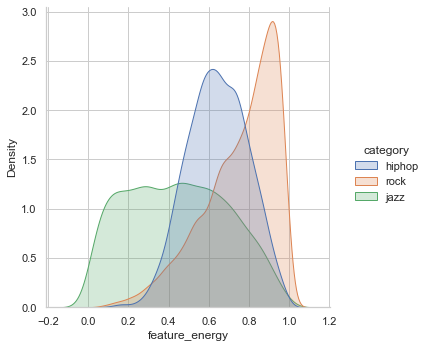
\includegraphics[width=4cm]{output_energy.png} }}%
    \qquad
    \subfloat[\centering Boxplot: \emph{energy}]{{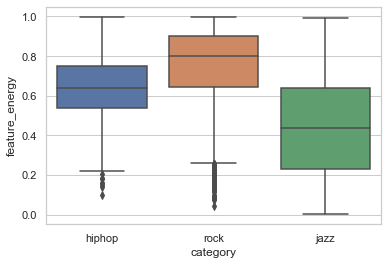
\includegraphics[width=4cm]{output_energy_boxplot.png} }}%
    \caption{\emph{energy} compared in the different categories}%
    \label{fig:du_dp_bp_enrg_categorie_dependent}%
\end{figure}

If we now look at the data in a distribution plot (\ref{du_dp_bp_enrg_categorie_dependent}}),
we see clear differences between the categories.
\emph{jazz} spreads over the whole graph but has no high point.
This can be attributed to the different types of \emph{jazz} (slow \emph{jazz}, free \emph{jazz}),
which means that different subtypes have different levels of energy.
Surprisingly, \emph{hiphop} is also broadly positioned and sets the high point at about \(0.61\).
\emph{hiphop} also has many facets as a genre, which is why this expression also makes sense.
The curve of \emph{rock} builds up early but rises very steeply in the last third of the graph and marks
its high point at about \(0.9\). 

After these three sample features, some more distributions and boxplots are added to better
explain the characteristics of the individual genres.

\begin{figure}[H]
    \centering
    \subfloat[\centering Distribution plot: \emph{Speechiness}]{{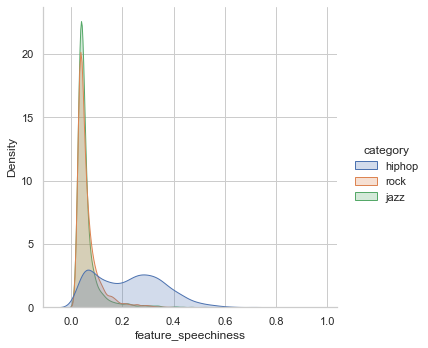
\includegraphics[width=4cm]{output_Speechiness.png} }}%
    \qquad
    \subfloat[\centering Boxplot: \emph{Speechiness}]{{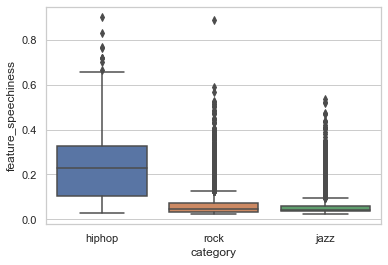
\includegraphics[width=4cm]{output_Speechiness_Boxplot.png} }}%
    \qquad
    \label{fig:du_ds_bp_speechiness}%
\end{figure}

\begin{figure}[H]
    \centering
    \subfloat[\centering Distribution plot: \emph{danceability}]{{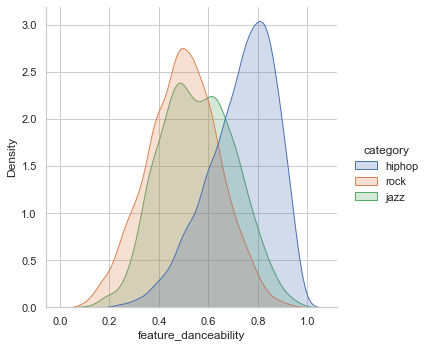
\includegraphics[width=4cm]{output_Danceability.png} }}%
    \qquad
    \subfloat[\centering Boxplot: \emph{danceability}]{{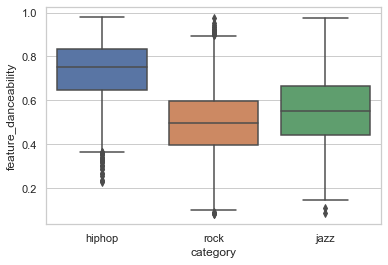
\includegraphics[width=4cm]{output_Danceability_Boxplot.png} }}%
    \qquad
    \label{fig:du_ds_bp_danceability}%
\end{figure}

\begin{figure}[H]
    \centering
    \subfloat[\centering Distribution plot: \emph{accousticness}]{{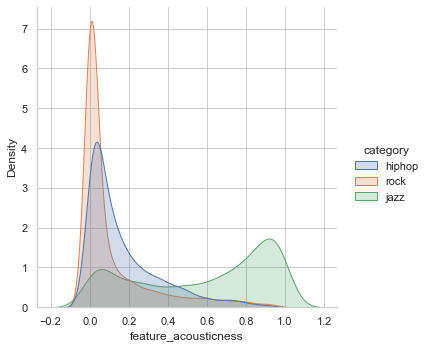
\includegraphics[width=4cm]{output_accousticness.png} }}%
    \qquad
    \subfloat[\centering Boxplot: \emph{accousticness}]{{\includegraphics[width=4cm]{output_accousticness_Boxplot.png} }}%
    \qquad
    \label{fig:du_ds_bp_accousticness}%
\end{figure}

\begin{figure}[H]
    \centering
    \subfloat[\centering Distribution plot: \emph{valence}]{{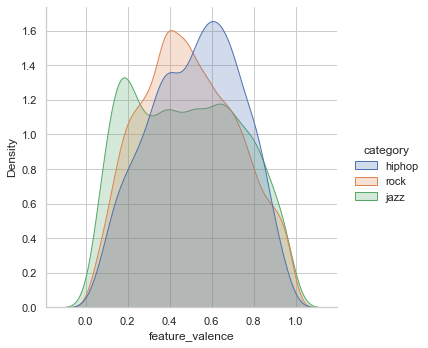
\includegraphics[width=4cm]{output_valence.png} }}%
    \qquad
    \subfloat[\centering Boxplot: \emph{valence}]{{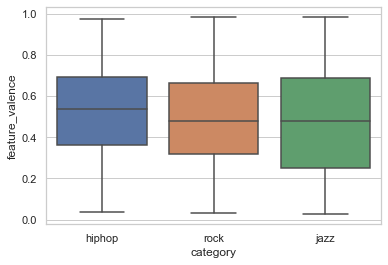
\includegraphics[width=4cm]{output_valence_Boxplot.png} }}%
    \qquad
    \caption{Different features visualized in distribution- and boxplots}%
    \label{fig:du_ds_bp_valence}%
\end{figure}
\subsection{Data Preparation}
\label{sec:Data Preparation}

In the following section the data is prepared and cleaned up for training the model.

Data preparation is done in Python using multiple libraries. The same libraries
are also used in the modeling and evaluation stages of this project.
\emph{pandas} is used for storing and manipulating data in dataframes.
\emph{sklearn} is used for splitting data, creating validation curves,
transforming data and training the gradient boosting model.
\emph{matplotlib} and \emph{seaborn} are used for data visualization and plotting.
Additionaly \emph{numpy} is used for other operations on the data.

As with data collection, the complete code with documentation is attached in the appendix.

\subsubsection{Import and Cleaning}


The CSV file is first imported and converted into a pandas dataframe.

\begin{lstlisting}[language=Python]
    df_import = pd.read_csv(os.path.join('..', 'data_collection', 'final_result.csv'))
\end{lstlisting}

Next, duplicates are removed. If there are two or more datapoints, which have the same value in their artist
and name column, only the first one is kept and all subsequent entries are removed.
This deduplication could also be done by using track ids. The drawback of this method is, that many artists
release their tracks multiple times, e.g. as a single and later in an album. These duplicates would not be
caught using the id, as different releases have different id values. As the artist and title doesn't change, almost
all duplicates are caught using artist and name.

\begin{lstlisting}[language=Python]
    df_dedup = df_import.drop_duplicates(subset=['categories.playlists.tracks.artists', 'categories.playlists.tracks.name'])
\end{lstlisting}

Next, all genres that are not to be used for training the model are filtered out.

\begin{lstlisting}[language=Python]
    genre_filter = ['hiphop', 'jazz', 'rock']
    df_filtered = df_dedup[df_dedup['categories.id'].isin(genre_filter)]
\end{lstlisting}

Then columns that are not needed for training are removed, including category name, all playlist information and
all track and album information. The category id is kept, as it will serve as the label.
The remaining columns are renamed, as the long JSON tree names are no longer needed.
The field \emph{category.id} is renamed to \emph{category} and each audio feature is renamed for example 
the danceability column is now called \emph{feature\_danceability}.
With unnecessary columns removed, a check is done to show any remaining null values.

\begin{lstlisting}[language=Python]
    df.isnull().sum()
\end{lstlisting}

In this dataset, there are no null values present.

The \emph{GradientBoostingClassifier} used for modeling only supports integer values as label input.
The category data is therefore encoded with integers using a custom function \emph{encode\_target}.
It takes a dataframe and the label column's name, than adds a "target" column with corresponding integer mappings.

\begin{lstlisting}[language=Python]
    def encode_target(df, target_column):

        df_mod = df.copy()
        map_to_int = {name: n for n, name in enumerate(df_mod["category"].unique())}
        df_mod["target"] = df_mod[target_column].replace(map_to_int)

        return (df_mod)

    df_target = encode_target(df, "category")
\end{lstlisting}

The head of the resulting dataframe is shown in table \ref{tbl:Dataframe after cleanup}.
The category to target integer mapping is shown in table \ref{tbl:Categories mapped to Integer Targets}.

\begin{table}[H]
    \begin{tabular}{l|rrrr}

    \toprule
    row & 0 & 1 & 2 & ... \\
    \midrule
    category & hiphop & hiphop & hiphop \\
    target & 0 & 0 & 0 \\
    feature\_danceability & 0.649 & 0.849 & 0.793 \\
    feature\_energy & 0.508 & 0.631 & 0.481 \\
    feature\_key & 8 & 3 & 9 \\
    feature\_loudness & -10.232 & -4.241 & -9.258 \\
    feature\_mode & 1 & 0 & 1 \\
    feature\_speechiness & 0.0959 & 0.0637 & 0.1240 \\
    feature\_acousticness & 0.03450 & 0.17100 & 0.01900 \\
    feature\_instrumentalness & 0.000036 & 0.000000 & 0.000001 \\
    feature\_liveness & 0.0736 & 0.1490 & 0.1390 \\
    feature\_valence & 0.405 & 0.550 & 0.395 \\
    feature\_tempo & 157.975 & 135.997 & 132.202 \\
    feature\_duration\_ms & 194051 & 215304 & 2046526 \\
    feature\_time\_signature & 4 & 4 & 4 \\
    \bottomrule
%
%    {} & category &  target &  feature\_danceability &  feature\_energy &  feature\_key &  feature\_loudness &  feature\_mode &  feature\_speechiness & \\
%    0 &   hiphop &       0 &                 0.649 &           0.508 &            8 &           -10.232 &             1 &               0.0959 &       \\
%    1 &   hiphop &       0 &                 0.849 &           0.631 &            3 &            -4.241 &             0 &               0.0637 &       \\
%    2 &   hiphop &       0 &                 0.793 &           0.481 &            9 &            -9.258 &             1 &               0.1240 &       \\
%    3 &   hiphop &       0 &                 0.875 &           0.478 &            7 &           -10.562 &             1 &               0.2180 &       \\
%    4 &   hiphop &       0 &                 0.684 &           0.624 &            2 &            -7.414 &             0 &               0.3470 &       \\
%    5 &   hiphop &       0 &                 0.762 &           0.649 &           11 &            -5.624 &             0 &               0.0527 &       \\
%
%    {} &  feature\_acousticness &  feature\_instrumentalness &  feature\_liveness &  feature\_valence &  feature\_tempo &  feature\_duration\_ms &  feature\_time\_signature \\
%    \midrule
%    0 &         0.03450 &                  0.000036 &            0.0736 &            0.405 &        157.975 &               194051 &                       4 \\
%    1 &         0.17100 &                  0.000000 &            0.1490 &            0.550 &        135.997 &               215304 &                       4 \\
%    2 &         0.01900 &                  0.000001 &            0.1390 &            0.395 &        132.202 &               204626 &                       4 \\
%    3 &         0.00717 &                  0.000000 &            0.1470 &            0.409 &        128.990 &               200959 &                       4 \\
%    4 &         0.23900 &                  0.000000 &            0.1120 &            0.708 &        146.925 &               156735 &                       4 \\
%    5 &         0.58000 &                  0.000017 &            0.0971 &            0.501 &        145.090 &               239146 &                       4 \\
%    \bottomrule
    \end{tabular}
    \caption{Dataframe after Cleanup}
    \label{tbl:Dataframe after cleanup}
\end{table}

%\begin{table}[H    
%    \centering%    \begin{tabular}{llrrrrrr}
%    \toprule
%    {} & category &  target &  feature\_danceability &  feature\_energy &  feature\_key &  feature\_loudness & ...\\ 
%    \midrule
%    0 &   hiphop &       0 &                 0.649 &           0.508 &            8 &           -10.232 & ...     \\ 
%    1 &   hiphop &       0 &                 0.849 &           0.631 &            3 &            -4.241 & ...     \\ 
%    2 &   hiphop &       0 &                 0.793 &           0.481 &            9 &            -9.258 & ...     \\ 
%    3 &   hiphop &       0 &                 0.875 &           0.478 &            7 &           -10.562 & ...     \\ 
%    4 &   hiphop &       0 &                 0.684 &           0.624 &            2 &            -7.414 & ...     \\ 
%    5 &   hiphop &       0 &                 0.762 &           0.649 &           11 &            -5.624 & ...     \\ 
%    \bottomrule
%    \toprule
%    ... & feature\_mode &  feature\_speechiness &  feature\_acousticness &  feature\_instrumentalness &  feature\_liveness &  feature\_valence &  feature\_tempo \\
%    \midrule
%    1 &               0.0959 &               0.03450 &                  0.000036 &            0.0736 &            0.405 &        157.975 &         
%    0 &               0.0637 &               0.17100 &                  0.000000 &            0.1490 &            0.550 &        135.997 &         
%    1 &               0.1240 &               0.01900 &                  0.000001 &            0.1390 &            0.395 &        132.202 &         
%    1 &               0.2180 &               0.00717 &                  0.000000 &            0.1470 &            0.409 &        128.990 &         
%    0 &               0.3470 &               0.23900 &                  0.000000 &            0.1120 &            0.708 &        146.925 &         
%    0 &               0.0527 &               0.58000 &                  0.000017 &            0.0971 &            0.501 &        145.090 &         
%\bottomrule
%
%      194051 &                       4 \\
%      215304 &                       4 \\
%      204626 &                       4 \\
%      200959 &                       4 \\bular}
%      156735 &                       4 \\
%      239146 &                       4 \\

%    \end{tabular}
%\end{table}

\begin{table}[H]
    \centering
    \caption{Categories mapped to Integer Targets}
    \label{tbl:Categories mapped to Integer Targets}
    \begin{tabular}{lr} 
        \toprule
        Category & Integer Target \\ [0.5ex]
        \midrule
        hiphop & 0 \\ [1ex]
        rock & 1 \\ [1ex]
        jazz & 2 \\ [1ex]
        \bottomrule
    \end{tabular}
\end{table}

Looking at the number of samples per category (table \ref{tbl:Number of Samples per Category after Cleanup}) reveals, that the dataset
is very uneven, with more than half of the samples falling into the category \emph{rock}.

\begin{table}[H]
    \centering
    \caption{Number of Samples per Category after Cleanup}
    \label{tbl:Number of Samples per Category after Cleanup}
    \begin{tabular}{lr} 
        \toprule
        Category & Number of Samples \\ [0.5ex]
        \midrule
        hiphop & 2694 \\ [1ex]
        rock & 7252 \\ [1ex]
        jazz & 3431 \\ [1ex]
        \bottomrule
    \end{tabular}
\end{table}

As explained in section \ref{sec:Mean Removal, Variance Scaling and Standardization} and \ref{sec:Dimension Reduction}
methods like standardization and \ac{PCA} can have a positive impact on the models accuracy.
Before finding the best model using hyperparameter tuning, the best form of input data is evaluated by transforming
the data in different ways and training a Gradient Boosting model using the default parameters specified in sklearn.
This way, the best form of input data can be found without the overhead of resource intensive grid search.

To be able to easily train models using different forms of input data, a method \emph{eval\_prep} was created,
which takes a dataframe, a list of all feature column names and the label column name. It then splits the dataframe
into train and test sets, trains a \emph{GradientBoostingClassifier} and returns a simple accuracy score.
This process is explained in depth in the modeling section.

First, the regular dataframe is used as input data, resulting in an accuracy score of $0.8505$.

\begin{lstlisting}[language=Python]
    score = eval_prep(df, features, "target")
\end{lstlisting}

\subsubsection{Data Transformation}

Next, mean removal, variance scaling and standardisation are attempted, by using the \emph{StandardScaler}
class from sklearn to transform the data. The code for standardization is shown below.
Mean removal and variance scaling use the same class with additional parameters.

\begin{lstlisting}[language=Python]
    X_s = df[features]
    y = df["target"]

    X_s = StandardScaler().fit_transform(X_s)

    df_s = pd.DataFrame(data=X_s)
    df_s.insert(0, "target", y)
    df_s.columns = ["target"] + features

    score = eval_prep(df_s, features, "target")
\end{lstlisting}

This results in the following scores, beating the untransformed data in all cases.

\begin{itemize}
    \item Mean Removal: $0.8509$
    \item Variance Scaling: $0.8520$
    \item Standardization: $0.8523$
\end{itemize}

\subsubsection{Principal Component Analysis}

Next \ac{PCA} is attempted using sklearns \emph{PCA} class. It is able to take any dataset and reduce
its dimensionality to any number of dimensions. The dimensionality is reduced to all dimensions
between 2 and 13 to see, which dimensionality results in the best score.
\ac{PCA} was done both on the raw dataset and in combination with standardized data (both before and afterwards).

\ac{PCA} does not yield good results with this dataset. The score for all of the combination is always worse
than using untransformed data. 
The PCA score was best when keeping 13 dimensions, declining further when removing more dimensions.
These are the scores using each combination with PCA and keeping 13 dimensions:

\begin{itemize}
    \item PCA only with 13 components: $0.8352$
    \item Standardization after PCA with 13 components: $0.8348$
    \item Standardization before PCA with 13 components: $0.8277$
\end{itemize}

Figure \ref{fig:Score for each PCA dimensionality} shows the test accuracy using PCA on the untransformed data
for each number of components.

\begin{figure}[H]
    \caption{Test accuracy for each dimensionality after PCA}
	\label{fig:Score for each PCA dimensionality}
    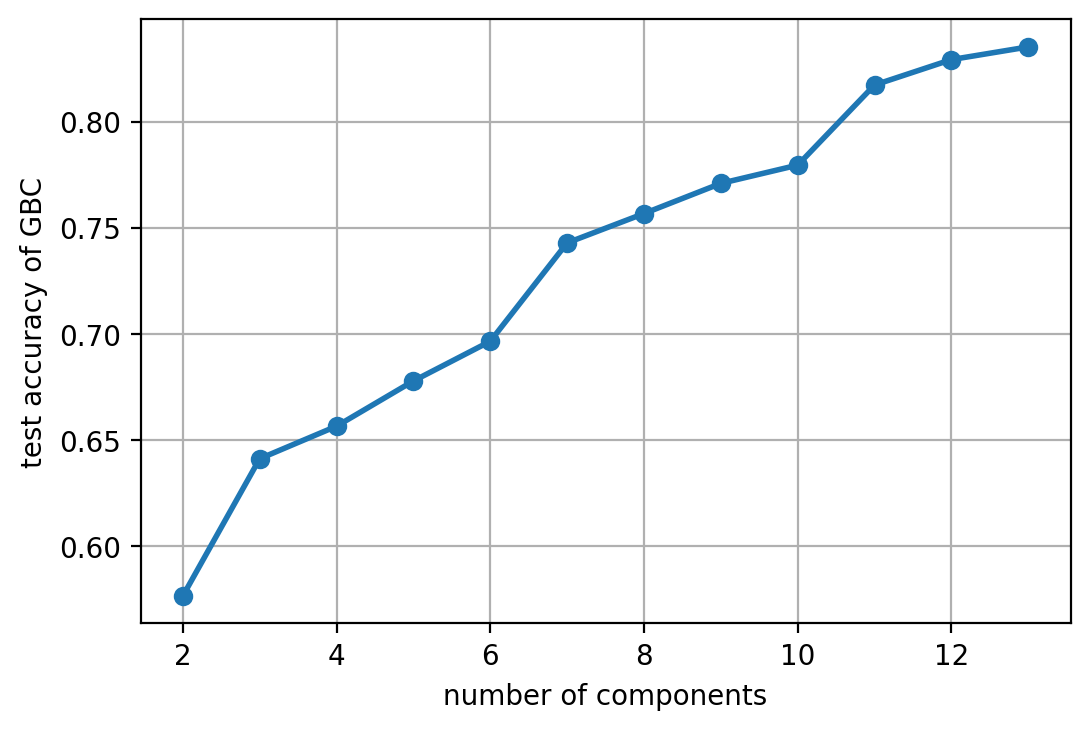
\includegraphics[width=0.6\textwidth]{dimensionality_PCA}
\end{figure}

As the results using \ac{PCA} do not improve the score, the code is not shown here.
Testing data transformation and dimension reduction with this dataset and a default \emph{GradientBoostingClassifier}
shows, that the model benefits slightly from standardized data, improving the overall score compared to the raw dataset
by $0.19\%$. Therefore, standardized data is used going forward.


%Now that all columns needed for training the model are prepared, the dataset needs to be split in 
%test and training data. This is necessary to be able to calculate an accuracy score for the model after training.
%In order to calculate this score, data is needed that the model has never seen before, which ensures that 
%the score is not just a result of overfitting, but the accuracy would be the same on real world data.
%For splitting the data, the function \emph{train\_test\_split} from sklearn is used.
%First the dataset is shuffled so each set contains a near equal amount of entries for each genre.
%Then the shuffled dataset is split, with an 80\% of samples going into the training set and 20\% going 
%into the test set. This results in 10.701 rows of training data and 2.676 rows of test data.
%
%\begin{lstlisting}[language=Python]
%    from sklearn.model_selection import train_test_split
%    df_target_shuffled = df_target.sample(frac=1, random_state=45)
%    train, test = train_test_split(df_target_shuffled, test_size=0.2, random_state=45, shuffle=False)
%\end{lstlisting}
%
%Next, features and labels are split into seperate datasets. This is necessary, because the GradientBoostingClassifiers
%fit method takes features and labels as seperate arguments called X for input and y for label. Datapoints are matched by their row numbers.
%Labels are stored in a list containing all values from the target column like so.
%
%\begin{lstlisting}[language=Python]
%    # y contains list of target values
%    y_train = train["target"]
%    y_test = test["target"]
%    y_all = df_target_shuffled["target"]
%\end{lstlisting}
%
%The features are stored in dataframes. The columns are selected using a list of all column names which contain features
%and then creating a new dataset only containing those columns:
%
%\begin{lstlisting}[language=Python]
%    # columns 1 to 14 contain the features, column 0 is the category and 15 the target
%    features = list(train.columns[1:14])
%
%    # create datasets only containing feature columns
%    X_train = train[features]
%    X_test = test[features]
%    X_all = df_target_shuffled[features]
%\end{lstlisting}
%
%At this point, all data has been cleaned up, targets have been generated, it has been split into training and test data and
%features have been seperated from labels. The data is now ready for training the model.
\subsection{Modeling}
\label{sec:Modeling}

\subsubsection{The Classifier}

For training the Gradient Boosting Algorithm, the \emph{GradientBoostingClassifier} class from 
the \emph{scikit} learn Python library is used. It is part of a group of classes offering different ensemble methods.
As explained in section \ref{sec:Gradient Boosting}, ensemble methods combine the predictions of several
weak learners to generate a more robust model and reduce overfitting issues.
\emph{sklearn} supports averaging methods like Bagging and Random Forests, which take the average of each learners prediction
as their output. It also supports Boosting methods like AdaBoost or Gradient Boosting, which
build base estimators sequentially, improving the output for each iteration.
\emph{sklearn} also provides a classifier and regressor model for each method.

The Gradient Boosting classifier supports binary and multi-class classification and uses
20 hyperparameters to control the size of each regression tree, the number of trees,
the learning rate and many more.
As explaining and tuning all 20 hyperparameters of the classifier would be beyond the scope of this
paper, three important parameters are explained and optimized.

\begin{itemize}
    \item \textbf{learning\_rate}
    
    As explained in section \ref{sec:Gradient Boosting Algorithm}, the learning rate is used to control how
    much each tree contributes to the result, by multiplying it with the output values of the previous 
    tree. The default value here is $0.1$.
    \item \textbf{n\_estimators}

    The number of weak learners (here regression trees) to be used while boosting. The default is $100$.
    \item \textbf{max\_depth}

    The maximum depth of each regression tree. This also impacts its number of nodes.
    The default value is $3$.
\end{itemize}

\subsubsection{Validation Curves}

During hyperparameter tuning, grid search is used to find the optimal value for each parameter.
As the computation is very resource intensive, a sensible range of values to search in must be found beforehand.
Validation curves can be used to observe how a model's score changes when modulating a single hyperparameter.
Here, an important distinction between the training and cross-validation score must be made.
The training score is the accuracy the model achieves when being scored on the same data it was trained on.
A very high training score could be a sign of overfitting.
The cross-validation score (cv score) is the mean accuracy achieved during 5-fold cross validation and is a good measure
of the actual performance of the model.

\begin{figure}[H]
    \centering
    \subfloat[\centering learning\_rate]{{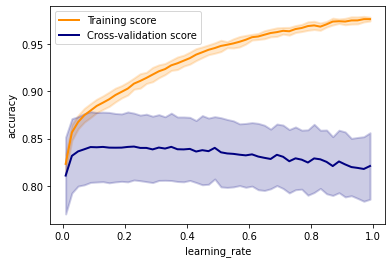
\includegraphics[width=0.45\textwidth]{validation_curve_learning_rate} }}%
    \qquad
    \subfloat[\centering n\_estimators]{{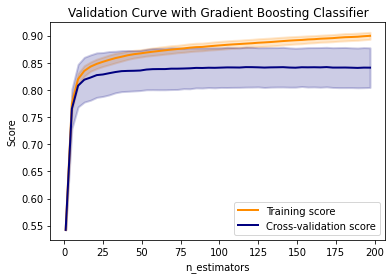
\includegraphics[width=0.45\textwidth]{validation_curve_n_estimators} }}%
    \qquad
    \subfloat[\centering max\_depth]{{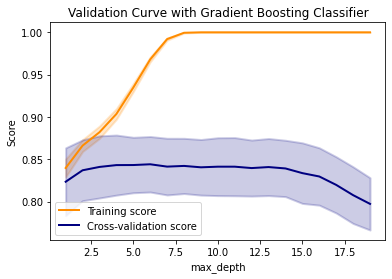
\includegraphics[width=0.45\textwidth]{validation_curve_max_depth} }}%
    \caption{Validation Curves modulating three Hyperparameters}%
    \label{fig:Validation Curves modulating 3 hyperparameters}%
\end{figure}

Figure \ref{fig:Validation Curves modulating 3 hyperparameters} shows the curves for each hyperparameter. The shaded
areas around the graph are the standard deviation, while the graph itself represents the mean score between 5 folds.

Figure \ref{fig:Validation Curves modulating 3 hyperparameters}a shows the best cv score with a learning rate
between $0$ and $0.2$, declining as it approaches one.
The training score rises as the learning rate increases, which indicates that the model becomes less generalizable and
more overfitted as the learning rate increases.
Because of these results, only values between $0.01$ and $0.25$ are considered during hyperparameter tuning.

The cv score stays relatively flat as the number of estimators goes beyond $25$ (figure \ref{fig:Validation Curves modulating 3 hyperparameters}).
The training score increases slightly.
This indicates that a training score close to, but above 25 might be optimal. As the results are not very clear,
a range between $50$ and $200$ is used for optimization.

For \emph{max\_depth}, the cv score stays relatively flat between $2$ and $13$ (figure \ref{fig:Validation Curves modulating 3 hyperparameters}).
The training score, on the other hand, increases rapidly from $0$ to $7.5$, where it reaches its maximum.
Because of this, a range between $2$ and $6$ is used for hyperparameter tuning.

\subsubsection{Hyperparameter Tuning and Fitting a Model}

The parameter grid is given as a Python dictionary containing the parameter name as keys and a list of values for
each key. All undefined hyperparameters are kept at default.
The grid used for training with the value ranges found above looks like this:

\begin{lstlisting}[language=Python]
    param_grid = {
        "learning_rate": [0.01, 0.04, 0.07, 0.1, 0.13, 0.16, 0.19, 0.22, 0.25],
        "n_estimators": [50, 75, 100, 125, 150, 175, 200],
        "max_depth": [2, 3, 4, 5, 6]
    }
\end{lstlisting}

The grid and a \emph{GradientBoostingClassifier} object are passed into a \emph{GridSearchCV} object
which executes the grid search using 5-fold CV.

\begin{lstlisting}[language=Python]
    gbc = GradientBoostingClassifier(random_state=45)    
    search = GridSearchCV(gbc, param_grid,
        n_jobs=-1,
        error_score="raise",
        verbose=1)
\end{lstlisting}

The search object's fit method combines cross-validation, hyperparameter tuning and classifier
fitting to find the best possible combination of hyperparameters to the estimator for the given dataset.
This is done in the following way:

\begin{enumerate}
    \item An estimator is created using the first combination of hyperparameters.
    \item The training set is split into five folds and each fold is used once for calculating accuracy,
    with the other four used for training. The average of the five scores is used as the final score for
    this specific set of parameters.
    \item The score is saved together with the parameters
    \item These steps are repeated with every possible combination of parameters from the 
    parameter grid. This results in a score for every set of parameters.
    \item As every model was fitted using the same method, it is clear that the model with the highest
    score is using the best hyperparameters. A new model is trained without cross-validation using all
    available training data, to create the final model.
\end{enumerate}

The complete standardized dataset is split in $80$\% train and $20$\% test data.
The samples are shuffled before splitting to ensure an even distribution of data.
Then features and labels are seperated for input into the classifier.

\begin{lstlisting}[language=Python]
    train, test = train_test_split(df_s, test_size=0.2, random_state=45, shuffle=True)

    X_train = train[features]
    X_test = test[features]
    y_train = train["target"]
    y_test = test["target"]
\end{lstlisting}

Then hyperparameter tuning and estimator fitting is started using the training features and labels.

\begin{lstlisting}[language=Python]
    search.fit(X_train, y_train)
\end{lstlisting}

The parameter grid above has $315$ possible combinations. As each is fitted on five sets of folds,
there are $1575$ models fitted in total during this process.

The resulting model with the best cross-validation score used the following parameters:
\begin{itemize}
    \item learning\_rate: $0.1$
    \item n\_estimators: $100$
    \item max\_depth: $3$
\end{itemize} 

Calculating the accuracy of the resulting model using the test set resulted in an accuracy score of $0.8591$.

A weakpoint of the parameter grid used is that the values for \emph{n\_estimators} are spread by increments of $25$,
leaving possible room for improvement.
To check whether the model could be improved another parameter grid was used:

\begin{lstlisting}[language=Python]
    param_grid = {
        "learning_rate": [0.01, 0.04, 0.07, 0.1, 0.13, 0.16, 0.19, 0.22, 0.25],
        "n_estimators": [97, 98, 99, 100, 101, 102, 103],
        "max_depth": [2, 3, 4, 5, 6]
    }
\end{lstlisting}

This did not deliver a better result.

Even though a broad spectrum of values was given in the search grid, the optimal values 
are equal to the default parameters for the estimator set by \emph{sklearn}.
This might suggest that the developers set the default values using a similar dataset to the one used in this project.

Although many combinations were evaluated, there is still a possibility, that the best result found using the methods
explained in this section is only a local maximum and not actually the best solution.
A set of hyperparameters far different from the ones tested here, might lead to even better results.
\subsection{Evaluation}

After the completion of the modelling phase, the next step is to evaluate the results. The evaluation is split into 
the evaluation of the model itself followed by the evaluation of the overall process. 

\subsection{Gradient Boosting Evaluation}

In this section the Gradient Boosting Algorithm will observed in more detail by the most common metrics. Additionally, it also
will be compared with the much simpler Classification Tree Algorithm to highlight commonalities and different approaches between 
the two algorithms and create an all-encompassing picture for Gradient Boosting. 

The overall accuracy measured is around 86\%. This result is already positive as the Gradient Boosting Algorithm outperforms 
the Classification Tree, which achieves an also respectable 80\% accuracy. However, the accuracy score can only be used as a
fundamental basis for evaluating the overall performance with many unknowns that need to be worked through.

The first step of a deeper analysis is to create a confusion matrix for all categories. The confusion matrix is an approach of 
visualizing the performance by clustering the the output. The x1-axis represents the predicted values for the classes 
while the x2-axis stands of actual (correct) values \cite[p.235]{Davis_2006}. For this analysis three numbered classes 1 to 3 are necessary that 
typify the categories hiphop, rock and jazz in the stated order. The confusion matrix reveals two types of correct predictions and 
also two types of errors displayed in figure x. The confusion matrix for the Gradient Boosting Model is shown in figure x2.

The confusion matrix reveals four combinations of predicted and actual values (1). For Gradient Boosting the confusion matrix looks 
like the following (3).

(1) confusion matrix theory 

\begin{table}[H]
  \centering
  \begin{tabular}{lrrrr}
    \toprule
    predicted & class 1         &  class 2          \\
    actual    &                 &                   \\
    \midrule
    class 1   &  true positive  &  false negative   \\
    class 2   &  false positive &  true negative    \\
    \bottomrule
    \end{tabular}
  \caption{Evaluation: Confusion Matrix}%
  \label{tbl:evaluation_confusion_matrix}%
\end{table} 

\begin{table}[H]
  \centering
  \begin{tabular}{lrrrr}
    \toprule
    predicted &    0 &     1 &    2 &   all \\
    actual &      &       &      &       \\
    \midrule
    0      &  438 &    68 &   19 &   525 \\
    1      &   41 &  1307 &  122 &  1470 \\
    2      &   30 &   115 &  536 &   681 \\
    all    &  509 &  1490 &  677 &  2676 \\
    \bottomrule
    \end{tabular}
  \caption{Evaluation: Gradient Boosting Confusion Matrix}%
  \label{tbl:gb_confusion_matrix}%
\end{table} 

Visually, the highest misclassification takes place between classes jazz and rock while the lowest missclassification occurs
between hiphop and jazz. This result however has little significance, since the number of rock tracks, with a total of over 
1400, is significantly larger than the amount of both rock and jazz tracks. An evaluation based on absolute numbers would lead to 
misleading results partly due to the imbalance of the dataset. 

A better approach is to look at the following metrics which can be derived form the confusion matrix for every category \cite[p.235]{Davis_2006} (3). 

\(precision\;= \;\frac{true\:positive}{true\:positive\;+\;false\:positive}\)

\(recall\;= \;\frac{true\:positive}{true\:positive\;+\;false\:negative}\)

\(f1-score\;= \;\frac{precision\;*\;recall}{precision\;+\;recall}\)

\begin{table}[H]
  \centering
  \begin{tabular}{lllll}
    \toprule
    classes & precision & recall & f1-score & support \\
    \midrule
     hiphop &      0.86 &   0.83 &     0.85 &     525 \\
       rock &      0.88 &   0.89 &     0.88 &    1470 \\
       jazz &      0.84 &   0.79 &     0.79 &     681 \\
    \bottomrule
    \end{tabular}
  \caption{Evaluation: Gradient Boosting Classification Report}%
  \label{tbl:gb_classification_Report}%
\end{table} 

Precision and Recall are both performance metrics with different objectives. While precision is a measure of how many of the 
predicted elements for a class were correct, recall measures how many elements of a category were detected. It can be observed that 
the precision is high across all categories with rock being classified best with 12\% false-positive predictions while 
the false-positive rate for jazz was worst with over 21\%. Interestingly the results for recall are very similar with the model 
performing best for the category rock with an recall of 0.89 and again worst for jazz with 0.79. Hiphop is for both metrics in 
between of both extremas at around 0.85. 

The f1-score is a combination out of precision and recall and an attempt of capturing both metrics in a single value. Therefore
the results are not surpising. Jazz performed worst with only 0.79 while rock was classified best with 0.88 according to the 
f1-score. 

In conclusion all scores can be evaluated as positive outputs without any negative and unexplainable abnormalities. Also in comparison 
to decision trees a clear improvement of the results can be seen. The reason that jazz is ranked worst while rock reaches the 
highest values may be due to several reasons. One possible explanation can be found by reviewing the findings from the Data 
Understanding chapter. it it recognizable that the value-ranges for the features of jazz were significantly more distributed 
than for both rock and jazz and often without any high points. In addition, the value ranges of rock were often different from 
those of hip-hop and jazz, which simplifies classification. 

Another measure to evaluate a models performance is to plot its Reciver Operating Characteristics. The ROC is a plot of the true-positive
rate for the x1-axis and the false-positive rate on the x2-axis for every possible threshold. The benefit of ROC is that it plots the 
misclassification for every threshold while other metrics rely on a single threshold. Often there are also requirements for 
models in which the overall accuracy plays a subordinate role, such as that all samples of class X must be detected. The ROC helps 
to visualize such problems to find optimal solutions. A model whose results are close to the diagonal classifies data worse than a 
model whose curve is as close as possible to the point (0/1) in the coordinate system. This performance is often measured by means of 
the AUC, which is derived directly from the ROC. With help of the AUC comparability between models is possible. The ROC and AUC for 
the project are shown in figure X (sklearn + theroy).

  \begin{figure}[H]
    \centering
    \subfloat[\centering Gradient Boosting]{{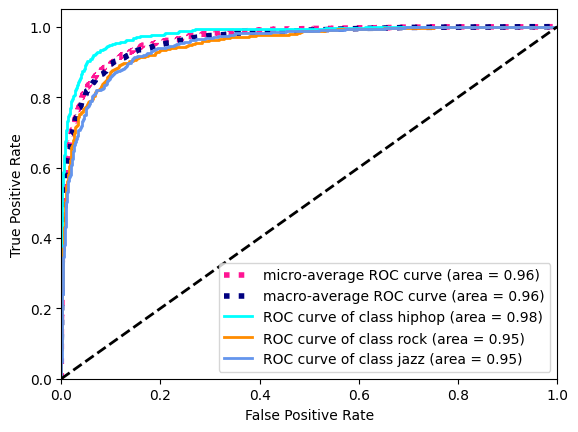
\includegraphics[width=6cm]{gb_roc_and_auc.png} }}%
    \qquad
    \subfloat[\centering Classification Tree]{{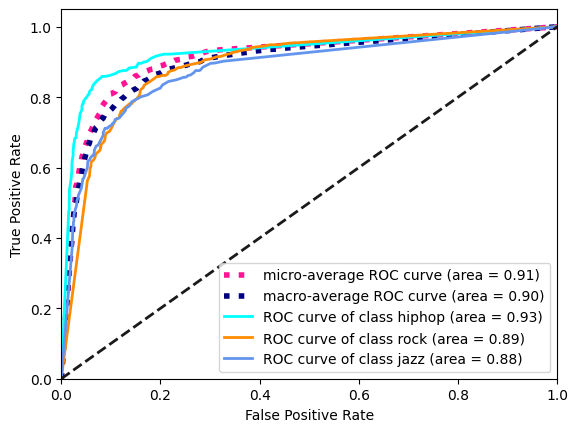
\includegraphics[width=6cm]{dt_roc_and_auc.png} }}%
    \caption{Evaluation: Comparison of ROC and AUC}%
    \label{fig:roc_and_auc_for_gb_and_dt}%
\end{figure}

From the following matrix it can be seen that the model works well for all classes. Both ROC and the associated AUC are convincing 
in all cases. What is interesting is the fact that rock has the worst AUC while being classified best according to the previous metrics.
Hiphop on the other hand has the significantly best AUC followed by jazz. An explanation for this result is complicated, with a 
possible reason again being the imbalance of the dataset. The model is focussed classifing rock correctly as it constitutes to a large part of the 
dataset. Therefore the optimum for both jazz and hiphop are exchanged for an overall optimum. It is noted that a well founded 
explanation would require more in-depth analysis. Regardless, the result is worth including in the analysis and leaves room for 
further research.   

In addition, a very different evaluation can be performed. It is also interesting to take a closer look on the input data with help of 
the so-called feature importance. The feature importance is a measure of how much impact a feature had for the classification of the 
dataset and is presented in the following figure for both Gradient Boosting and Decision Trees (sklearn). 

\begin{figure}[H]
  \centering
  \subfloat[\centering Gradient Boosting]{{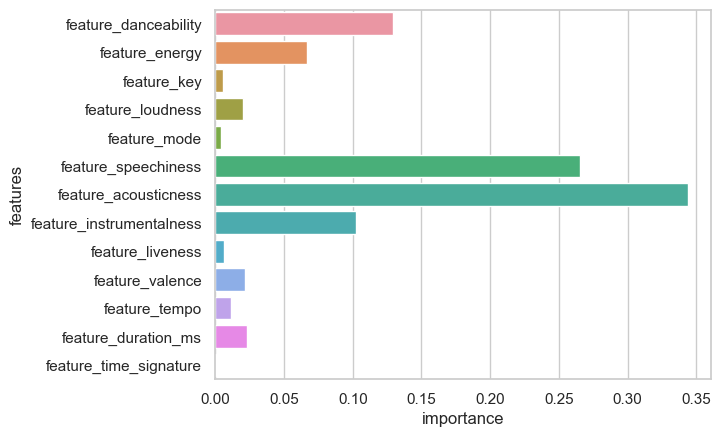
\includegraphics[width=6cm]{gb_feature_importance.png} }}%
  \qquad
  \subfloat[\centering Classification Tree]{{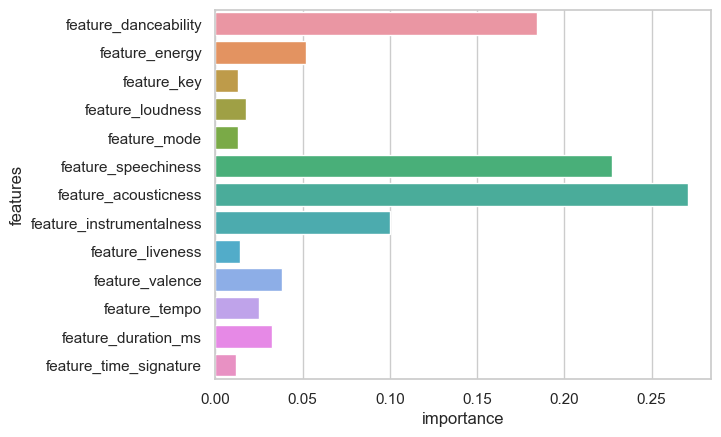
\includegraphics[width=6cm]{dt_feature_importance.png} }}%
  \caption{Comparison of Feature Importance}%
  \label{fig:feature_inportance_for_gb_and_dt}%
\end{figure}

It is clearly visible that both Gradient Boosting and Decision Trees relied on similiar features to similar extends for the classification task with 
minor differences for features such as danceability. Noticeable is that Gradient Boosting is heavily focused on a few features 
while the Classification Tree makes more use out of features like duration, valence and mode. One possibility for the difference in weighting  
could be the overall construction of the algorithms. Gradient Boosting consists out of multiple small weak learners while the Classification Tree
Algorithm froms a widely branched and deep tree. For feature importance again an analogy can be made to Data Understanding and the Music Theory. 
The features that theoretically distinguish the genres from another play the most important role for the modeling while musical standards and 
more subjective featues only play a subordinate role. This result is positive both for theory and the Machine Learning Model. The result states 
that music theory can be confirmed by real-world examples while giving credibility and plausibility to the model.

\subsection{Process Evaluation}

The evaluation of the overall process is complicated as there are many unknowns starting with the data itself. The data used is preprocessed by 
Spotify without detailed definition and theoretical basis. The features are furthermore heavily subjective which adds another layer of 
complexity. Also the data collection is non-trivial and error-prone. Both the collection process itself and the collection approach 
would have to be revised for a productive use case. On the other hand the data quality is decent with high correlation to the music 
theory. In addition the dataset convinces with its uniqueness and novelty.

The model in combination with the preprocessing and evaluation also leaves room for further research. The use of only two very 
similar Machine Learning Algorithms allows no comparison to completely differnt approaches based on other algorithms and concepts. 
It can therefore not be ruled out that even better results can be achieved. The pre-processing is intensive with many constallations 
tested. A possible improvement would be to apply the hyperparametric optimization not only on the standardized data but on all 
approaches to ensure the overall best result. In addition, there are further hyperparameter constellations which were not tested.
The evaluation may also have reached incorrect conclusions and assumptions for a variety of reasons. 

The overall highest risk is the fact that all participants of the group are not familiar with the Machine Learning and lack in 
experience. For this reason, the result can be considered promising. 


Daten:

- vorprozessiert von Spotify
- oft auch interpretation und subjektiv
- keine eindeutige Definition, was Aussagekraft schwierig macht
- Datensammlung -> Ungenau, fehleranfällig, jedoch gute und sehr interessante Datenbasis

Modelle:

- Korrektes Modell gewählt? -> kein Vergleich 

Vorprozessierung, Klassifikation und Auswertung: 

- hyperparameter nur auf standardized 
- Mehr optionen zu hyperparameter
- Evaluation und Schlüsse korrekt? -> Daten vielleicht nicht aussagekräftig
- Allgemein viel selbstgeschriebenes Coding -> fehleranfällig, da neu in Materie

\section{Conclusion}

- Ziel dieser Arbeit 

    - Klassifikation mithilfe von Gradient Boosting 
    - Aus selbstgenerierten Daten -> Spotify

    - Ausprobieren > bestes Modell 

- Modell und Projekt liefern gute Ergebnisse 

    - Anfang mit Decision Trees und danach Gradient Boosting hat sich als guter weg erwiesen
        -> Basis mithilfe derer Gradient Boosting aufgebaut werden konnte 

    - Keine Optimierungsmethoden außer Standardisierung brachten keine Verbesserungen
        - interessant und deutet auf gute Datenbasis hin 
        - Eventuell falsche Implementation und Ansatz, da noch viele Details offen sind (wie bereits besprochen in Evaluation)

    - Modelle beruhen auf ähnlichen Features, die bereits mittels der Theorie ermittelt wurden. 
        - Wie gut Modelle sind und wie sehr theoretisches nachgebildet werden kann
        - lässt sich vermutlich auch auf andere Machine Learning Algorithmen anwenden 
            - Analyse von komplexen, nicht eindeutigen und subjektive Daten möglich mit guten Resultaten 

-   Persönliche Erkenntnisse
    - Trotz einfachem Modell und Daten an Grenzen des Projektrahmens gestoßen -> Anzahl Wörter, Zeit, Modelle, etc. 
        - Planung zu Beginn konnte nicht genau eingehalten werdne 

    - Der Prozess von Datensammlung zu Modell war nicht geradlinig, aber hat durchaus sehr gut funktioniert und zu den 
      gewünschten Resultaten geführt 

    - Implementation nicht so kompliziert ist und viel Freude bereitet
    - Praktische Projekte öffnen augen in vielerlei Hinsicht. 
    - Teamarbeit zwar teilweise anstrengend und komplexer war, aber auch mehr Ideen, Input und allgemein bessere Ergebnisse hervorbrachte 
        - keiner hatte bisher Erfahrung mit Machine Learning -> Unterstützung  + Zusammenarbeit (über eigene Teile hinweg)

        %Since the problems and the assessment of the project work have already been described to a large extent in the evaluation, 
        %this chapter focusses more on the organizational and personal conclusions we experienced. 

        The project had the purpose to classify a dataset with the help of a machine learning algorithm. With no restrictions on the choice of dataset and algorithm given, 
        a classification of genres based on Spotify Music data was selected as a project task. After an extended search, 
        no sufficient existing dataset was found and thus a new dataset had to be created. Even though the data collection was complex at times, 
        it proofed to be a good decision and convinces with its novelty. After testing and debating over various algorithms, gradient boosting was
        selected as the machine learning algorithm. Additionally, a classification tree was implemented as a reference point.

        Overall the result was successful, with an accuracy of nearly 87 percent, with all other evaluation metrics indicating to a similar positive performance.
        Interestingly, despite high optimization efforts, only standardization led to a better result with no other optimization method improving the quality of the model. 
        This could indicate either that these methods were implemented incorrectly, or that the quality of the dataset was very high from the beginning. 
        The latter is supported by the fact that both algorithms classified the songs according to similar features as stated in theory to distinguish between genres.

        Personally, several lessons were learned from this project. The first lesson is, that despite only focussing on a 
        simple machine learning algorithm, the limits of the project framework were reached. Both in terms of the scope and size of the
        paper itself and from a algorithm implementation perspective, as mulitple optimization possibilites and design choices were 
        discovered while implementing and had to be addressed further. This goes hand in hand with the fact that the project execution was not straight-forward.
        With multiple changes and additions to the paper as well as implementations made along the way which shaped the 
        project into its final form. However, all changes should in no way be seen as negative, as they have led to the desired result and 
        are part of the learning process.
        Secondly, teamwork was required to manage a project of this size. The topics and chapters were assigned in advance, with constant exchange 
        of information on different issues and collaboration on topics such as data collection and model implementation.
        Thirdly, the overall learning curve was very steep. No participant of this group had previous experience in machine learning.
        Nevertheless, it was possible to create a well working classification model which meets the pre-set conditions of the overall task.

        - mittlerweile unglaublich einfach sowas zu selbst ohne großen Aufwand zu erstellen

        In conclusion, Spotify is just one example of many modern applications that use Big Data analytics to capture and attempt to reflect the often subjective world in numbers. 
        What is particularly interesting here is how this is attempted, and to what extent it works. The success of the company, or the widespread use of the app, 
        show how well the Echo Nest works. Still, like the model shown here, the deciding attributes are the ones closer to numbers, like Accousticness or Speechiness. 
        Attributes such as Valence, which attempts to measure mood, plays a small role in genre assignment. However, this can, and will, change in the future. 
        The decoding of the personal feeling of the user is the next step to more, and above all more decisive data and in the broader sense of a better customer relationship. 
        So we can look forward with great interest to the further development of such use cases.



%\section{Introduction}

Spotify is a music streaming service and has established itself as the leader in this
market. Since its launch in 2006, the company has gained over 365 million users, of
which nearly 45 percent are subscribed to the chargeable premium service.
The ability to listen to almost any song a user might want with a quick search and
the click of a button is a great benefit streaming services have over regular music vendors
like iTunes. On the other hand, users might quickly get lost or feel overwhelmed by such
a large collection to choose from.
To guide users and help them find the music they want to listen to in a certain situations
Spotify uses a number of methods like premade playlists or categories for specific moods and
genres. But the biggest part of the user experience might certainly be the personalized
playlists, radios or artist and song recommendations.
To be able to have such a robust recommendation system, Spotify needs to understand each users
listening behaviour and have methods to predict, which music a user might also like depending
on their past usage.
Not just user data is important to gain this knowledge, but Spotify also needs to understand
how to categorize music itself and find ways to tell, which songs are alike and how they
relate to each other.
Big Data is essential to achieve this goal. Machine learning is used 
to analyze the music in their catalogue and create characteristics about it.
Spotify offers this data to the public, which is the basis for this project.

\subsection{Problem Definition and Goal}

The paper is set in the context of Big Data Analytics and is supposed to explain and implement
many concepts and processes found here.
The basic goal of the project is to develop a machine learning model based on a dataset.
During this process, general data mining stages, as layed out in the \ac{CRISP DM} standard,
must be theoretically explored, understood and practically implemented. This includes steps like data
preparation, model creation, or evaluation. Creating a model with a high accuracy is only a secondary
concern in this project. Instead gaining a solid understanding of data mining concepts is paramount.

To achieve this goal, Spotify song data is collected and an attempt is made to build a gradient boosting
algorithm, which is able to classify songs into different genres based on audio features.

\subsection{Structure and Methodology of the Assignment}

The paper is divided into four main sections, starting with the introduction, containing the problem statement, goal and overall structure.

The second section discusses fundamental concepts. This includes sorting this project into the larger context of Big Data,
explaining the algorithms used on a theoretical level and introducing further concepts which are used for data preparation and modeling.
Additionally, the \ac{CRISP DM} model is explained, which is the basic structure that implementation is based on.
Concluding the second section is an introduction to the use cases and funcionality of Web \acp{API} and a discussion of basic concepts
in music theory.

The third section begins with the data collection process and continues on with the practical implementation steps 
of understanding the dataset's features and labels in the context of Spotify's analysis, preparing and analyzing the data for modeling, creating a
gradient boosting classifier and finally evaluating the project results. This process is fundamentally based on the CRISP DM model.

The paper concludes with a summary of the insights gained and embedding the project into a broader context.

Facts presented as part of the paper's fundamental sections are derived from literature research using renowned book sources and
scientific papers. Additionally online articles were used to round out the research.
Most visualizations in this paper are made by hand using Python libraries such as seaborn and matplotlib.
The general approach during implementation is derived from the CRISP DM model also explained in literature.
For data collection and understanding Spotify's developer resources are used as a reference.
Documentation from Python libraries such as scikit learn is used extensively during the preparation, modeling and evaluation parts
of the project.

%Large amounts of data are collected from everyday activities on the platform, stored and
%finally analyzed using machine learning algorithms, to power the recommendation and
%classification process. 


%This Premium
%service comes at a subscription cost of nowadays 12,99C per month, giving the opportu-
%nity to listen to every song that is available at Spotify - this being ca. 70 million tracks from
%over 1,2 million Artists. [54]




%  Based on an existing framework for data science projects. Starts with selection of dataset ...
%- Task: Model development and evaluation using Spotify audio features to classify genres 
%- Simplification: Genre classification instead of specific user recommendations
%- Dataset could be freely chosen and Spotify data was selected
%- Goal is to gain a good understanding about data mining processes, the problems involved
%and possible solutions. The final accuracy of the model is only secondary. 
%
%
%
%
%
%The amount of data collected every day is growing uncompromisingly. Further Proliferation of the Internet, Social Networks, 
%Search queries and increasing networking of IoT devices and sensors means that the amount of data is growing exponentially. 
%To remain competitive in their respective markets, companies must be able to extract value from the large amount of data.
%A conzept that decisively supports companies in exactly this task is Big Data. Big Data encompasses the entire process of data collection to analyzing it
%When combined with machine learning, Big Data unfolds its full potential. The combination allows very large data sets to be processed, 
%which is incredibly valuable for companies. This enables companies to capture their macro and microenvironment in data and create deciding business value. 
%Due to its wide range of applications, this field offers opportunities for improvement for companies of all kinds. 
%Even companies from the entertainment industry, such as Spotify, Netflix or Disney are already using these practices to improve the services they offer, 
%to differentiate themselves from the competition and to make the customer experience unique. 
%Spotify for example uses Big Data to give its users an individual Discover Weekly Playlist which consists of thirty recommended songs for that user. 
%This project has the purpose to illustrate and solve a real-world big data-related problem that could also occur in a company's Value creation process. 
%For this purpose, algorithms are applied to the solution within a controlled framework. Based on the \ac{CRISP DM} process, the data used was first collected, analyzed, 
%and finally evaluated. The problem to be solved is classifying songs using pre-generated features provided by Spotify for each music track on their platform. 
%For the classification, predefined genres by Spotify are taken as categories.
%
%The final goal of this paper is to apply a gradient boosting algorithm to a dataset collected from Spotify. 
%This algorithm should be trained during the course of the project and be able to assign songs to selected genres in the final product. 
%Along the way, the basics of Big Data itself, but also the working models and processes used in the project/model should be presented 
%in their theoretical form and explained clearly. Since not explicitly given, the individual collection of data by means of a given API (written out) 
%in combination with own coding shall find place as part of the model in an extra step. 
%Additionally, this paper should cover all the steps of the \ac{CRISP DM} model, and furthermore be an example of how Big Data projects can be approached 
%and performed in this style of work. Besides the Coding, the mechanisms of the Spotify algorithm and the mechanisms inside Spotify as a company are 
%explicitly explained to guarantee an overall good understanding of the whole project.

%\newpage
\section{Informationen vom Thesis-Day} \label{infos}
Siehe auch Wissenschaftliches Arbeiten~\cite[S. 1]{Balzert.2008}. %ohne textcommands
Damit sollten alle wichtigen Informationen abgedeckt sein ;-)~\footcite[\vglf][\pagef 1]{Balzert.2008} %mit textcommands
Hier gibt es noch ein Beispiel für ein direktes Zitat\footcite[][\pagef 1]{Balzert.2008} %mit textcommands

\subsection{Pre-Anmeldephase}
\subsubsection{Vorüberlegungen}
Trichtermethode: Man beginnt mit der eigentlichen  Konklusion und überlegt dann, welche allgemeinen Teile dafür benötigt werden.

Welchen Mehrwert soll die Arbeit bieten \footnote{Diese Fu\ss note hat inhaltlich keinen Sinn. Es soll nur ein langer Text generiert werden, dass dieser Vermerk über zwei Zeilen reicht und bündig dargestellt wird.}? Auch darüber nachdenken, wie die Arbeit einen selbst weiter bringen kann. Studienverlauf prüfen. Welche Vorlesungen hat mich besonders interessiert? Wo liegen meine Stärken etc.

\begin{enumerate}
\item Themenfindung
\item Literaturrecherche
\item Gliederung/Motivationspapier erstellen
\item Betreuerauswahl (siehe Liste im \ac{OC})
\item Anmeldung (ab 141 Credits möglich)
\end{enumerate}

\subsubsection{Anregungen finden}
\begin{itemize}
\item \href{http://www.diplom.de}{www.diplom.de}
\item \href{http://www.hausarbeiten.de}{www.hausarbeiten.de}
\item Datenbanken aus Tools and Methods
\item etc.
\end{itemize}

\newpage
\subsection{Anfertigungsphase}
Die Anmeldung ist mittlerweile jeden Mittwoch möglich.
\begin{figure}[H]
\caption{FOM-Vorgaben zur Thesis im Online-Campus}
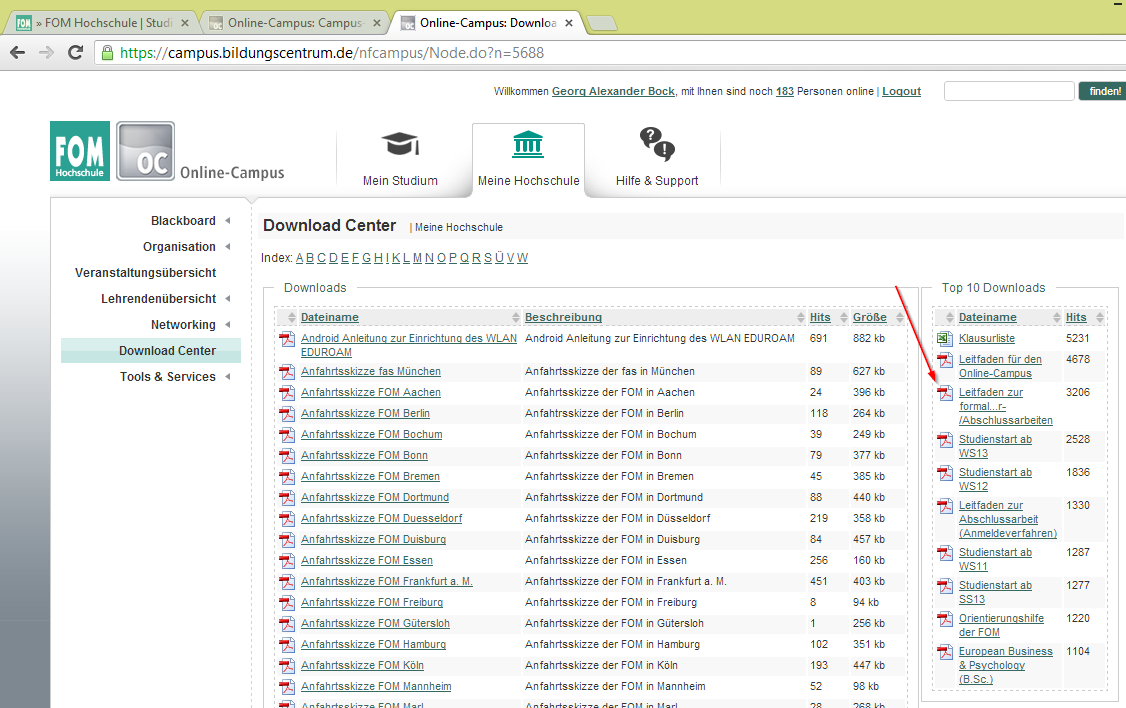
\includegraphics[width=0.9\textwidth]{campusDownload}
\\
\cite[Quelle: Vgl.][]{FOM}
\end{figure}

Laut Herrn Keller sollte der Umfang der Thesis (für eine gute Note) eher im Bereich der 60 Seiten liegen. Wie immer ist das vermutlich mit dem Betreuer abzustimmen. Die Liste der Dozenten, die Abschlussarbeiten betreuen, findet sich auch im \ac{OC}.

Zeit zur Erstellung der Thesis 2-4 Monate.

Es müssen zwei gedruckte Arbeiten abgegeben werden. Flüchtige Quellen als PDF ausgeben lassen und auf CD abgeben. Thesis zusätzlich digital einreichen. Beim Binden der Thesis auf Qualität achten. Haptik und erster Eindruck sind in der Bewertung \enquote{auch} wichtig. Arbeiten können in jedem FOM Studienzentrum abgegeben werden.

\subsection{Post-Abgabephase}
Nach Abgabe ca. 2 Wochen bis zum Kolloquium.

Kolloquium:
\begin{itemize}
\item Dauer: 30 Minuten
\item Präsentation (manche Prüfer wollen eine, andere nicht)
\item Betreuer vorher fragen was er möchte
\item Es gibt einen Frageteil, dieser bezieht sich auf die Arbeit, kann aber auch darüber hinaus gehen.
\item Der Tag des Kolloquiums steht auf der Endbenotung
\item Thesis und Kolloquium sind zwei getrennte Prüfungsbereiche. Für beide gibt es nur zwei Versuche.
\item Am Tag des Kolloquiums erhält man die Bestätigung, ob bestanden oder nicht
\end{itemize}

%\newpage
\section{Latex-Details} \label{latexDetails}

\subsection{Verwendete Software, Editor und Zusatzpakete}
\subsubsection{Windows 8+}
\begin{itemize}
\item MikTex: 2.9, 32-bit
\item Biblatex: 3.5, Zusatz: Biber.exe
\item Editor: TexStudio (kann ich empfehlen), Notepad++
\end{itemize}

\subsubsection{Mac OSX und iOS}
\begin{itemize}
\item MacTeX: \url{https://tug.org/mactex}
\item Editor: TexPad \url{https://www.texpadapp.com}
\end{itemize}

\subsubsection{Online}
Overleaf ist eine Online-Anwendung mit der Ihr direkt im Browser an eurer Thesis schreiben könnt. Bis 1GB Größe und maximal 60 Einzeldateien könnt ihr Overleaf kostenlos nutzen: \url{https://www.overleaf.com/}


\subsection{Dokumentenklasse}
Eigentlich hatte Prof. Finke empfohlen die Dokumentklassen \enquote{Book} oder \enquote{Report} für die Erstellung der Bachelor-Thesis zu verwenden, da diese über weitere Gliederungsebenen verfügen. Ich verwende dennoch eine leicht modifizierte Komaskript-Klasse \enquote{scrartcl}, mit der Erweiterung um eine Ebene. Siehe (skripte/weitereEbene.tex). Das Skript stammt irgendwo aus den Netz und übersteigt meine \LaTeX{}-Fähigkeiten. Dadurch kann ich über eine weitere Ebene in der Arbeit verfügen, ohne mich mit der Modifikation von Kapitel-Seiten rumschlagen~\footcite[Vgl. ][S. 5]{Tanenbaum.2003} zu müssen. Diese Quelle ist nur zur Demonstration und hat keinen inhaltlichen Bezug hierzu. Es werden übrigens nur die Quellen im Literaturverzeichnis angezeigt, die auch referenziert sind.


\subsection{Grafiken}
Das Paket \textbackslash usepackage\{float\} ermöglicht es die Grafiken und Tabellen an der Stelle im Text zu positionieren, wo diese im Quelltext stehen (Option H). Ansonsten würde \LaTeX{} diese dort unterbringen, wo es typographisch sinnvoll wäre - das wollen wir ja nicht ;-).

Die Breite der Grafiken am Besten relativ zum Text angeben.

\subsection{Quellcode}
Quellcode kann auf unterschiedliche Arten eingebaut werden.
Zum einen kann es hier durch direktives Einbinden in der Kapitel-Datei geschehen.
\begin{lstlisting}
% Hier wird aufgezeigt, wie man eine Grafik einbindet, es wird also in der PDF angezeigt,
% da es in einem Quellcode-Listing steht.
% Auch wenn es hier faelschlicherweise als LaTeX-Befehl angezeigt wird.
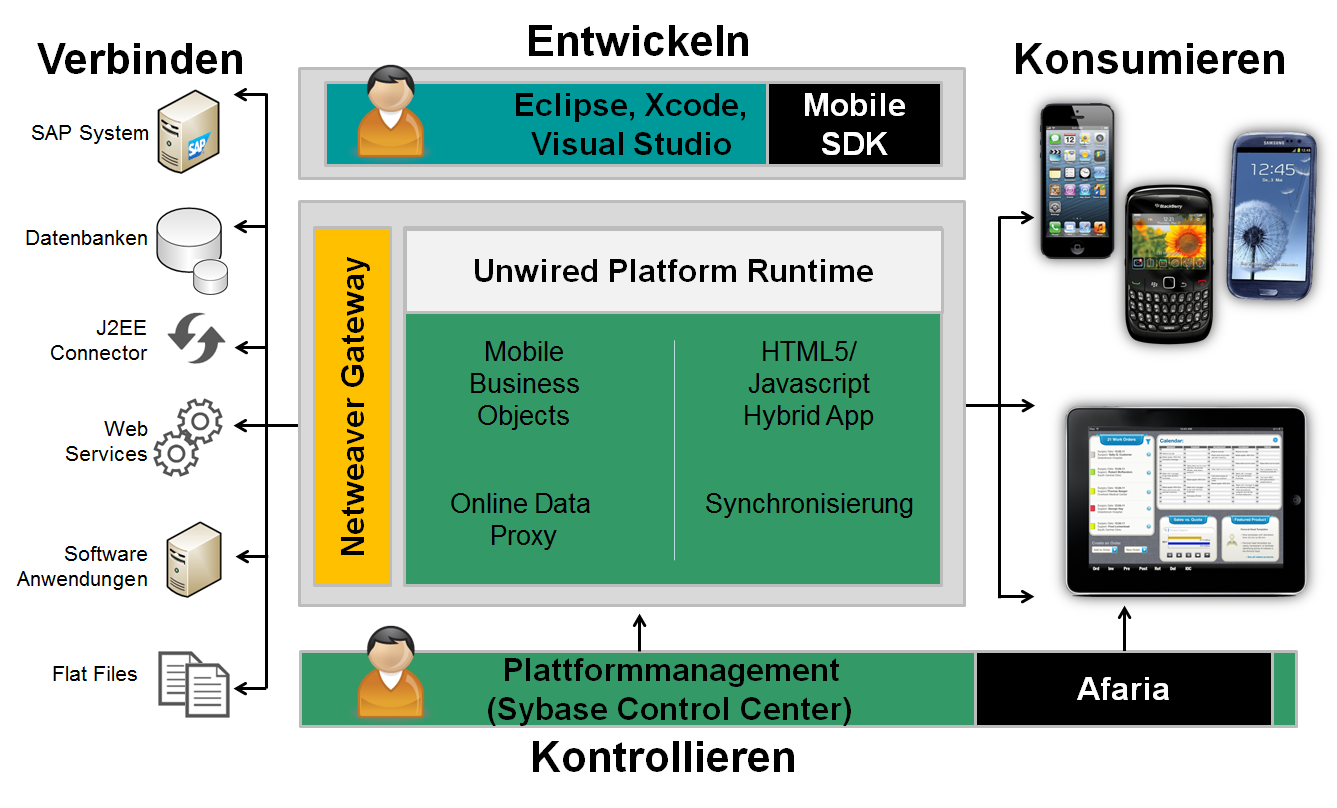
\includegraphics[width=0.9\textwidth]{sup}
\end{lstlisting}

Bei längeren Quellcode-Listings empfiehlt es sich jedoch auf eine externe Datei im Ordner Quellcode zu verlinken und diese einzubauen:
\lstinputlisting[language=HTML]{./source_code/Beispiel.html}

Statt dem Package lstlisting, welches direkt auf Tex basiert, kann auch das Package minted verwendet werden.
Dieses Package basiert auf python-pygments und unterstützt weit mehr Sprachkonstrukte als lstlisting.
Um das Paket zu verwenden muss es eingebunden werden und zusätzlich python-pygments installiert sein.
(Dies ist mit im Dockerfile vorhanden. Für die anderen Compile-Methoden, wie das native verwenden von Tex Live findet sich hier die Installationsanleitung für das minted Paket: https://ctan.org/pkg/minted?lang=de)

Damit das kompilieren ohne Python trotzdem möglich ist, ist die Funktion standardmäßig ausgebaut. Deshalb muss zusätzlich in der Datei \begin{verbatim}thesis_main.tex \usepackage{minted} \end{verbatim} wieder einkommentiert werden. 

Minted lässt sich dann ganz ähnlich zu lstlisting verwenden:
\begin{lstlisting}
	\begin{minted}{c}
		int main() {
			printf("hello, world");
			return 0;
		}
	\end{minted}
\end{lstlisting}	

Da der Pfad zu den Abbildungen im Hauptdokument definiert wurde, muss hier nur noch der Name des Bildes ohne Dateiendung stehen (sup).

\begin{figure}[H]
\caption{Titel der Abbildung hier}
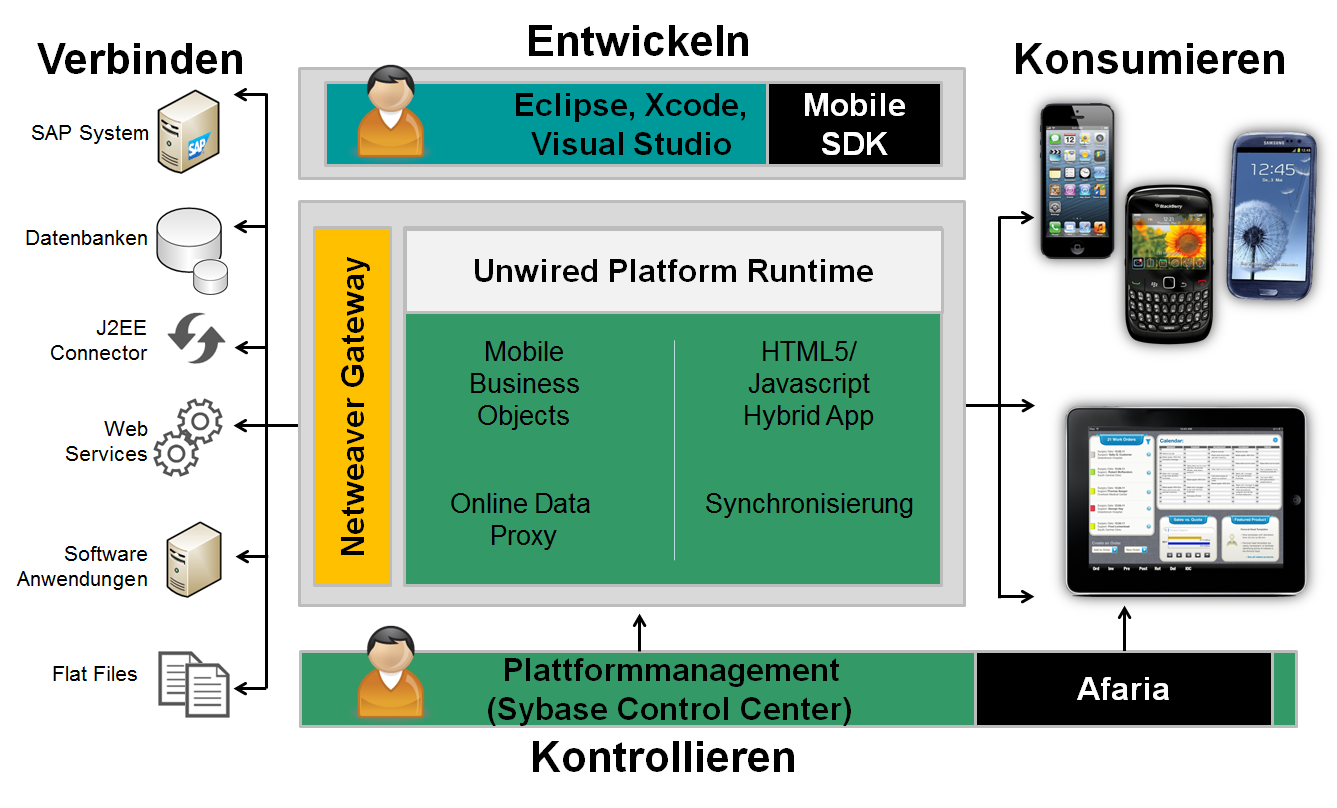
\includegraphics[width=0.9\textwidth]{sup}
\\
Quelle: Eigene Darstellung
\end{figure}

\subsection{Tabellen}
\begin{table}[H]
\caption{Beispieltabelle 1}
\label{tbl:beispieltabelle2}
\begin{tabularx}{\textwidth}[ht]{|l|X|l|}
  \hline
  \textbf{Abkürzung} & \textbf{Beschreibung} & \textbf{Berechnung}\\
  \hline\hline
    MEK & Materialeinzelkosten & \\
  	MGK & Materialgemeinkosten & $+ \uparrow$~*\\
    FEK & Fertigungseinzelkosten & \\
  	FGK & Fertigungsgemeinkosten & $+ \uparrow$~*\\
	SEKF & Sondereinzelkosten der Fertigung & \\
	\hline\hline
	\multicolumn{3}{|l|}{\textbf{= Herstellungskosten}} \\
	\hline\hline
  	VwGK & Verwaltungsgemeinkosten & $+ \uparrow$~*\\
  	VtGK & Vertriebsgemeinkosten & $+ \uparrow$~*\\
  	SEKVt & Sondereinzelkosten des Vertriebes & \\
	\hline\hline
	\multicolumn{3}{|l|}{\textbf{= Selbstkosten}} \\
	\hline\hline
	\multicolumn{3}{|l|}{+ Gewinnaufschlag} \\
	\multicolumn{3}{|l|}{+ Rabatte} \\
	\hline\hline
	\multicolumn{3}{|l|}{\textbf{= Nettoverkaufspreis (NVP)}} \\
	\hline
	\multicolumn{3}{|l|}{+ Umsatzsteuer} \\
	\hline\hline
	\multicolumn{3}{|l|}{\textbf{= Bruttoverkaufspreis (BVP)}} \\
	\hline
\end{tabularx} \\
\cite[Quelle: In Anlehnung an][S. 4]{Beckert.2012}
\end{table}

%\clearpage % hiermit werden alle Bilder Tabellen ausgeworfen

\subsection{Biblatex}
\subsubsection{Erklärung}
Von den vielen verfügbaren Literatur-Paketen habe ich mich für Biblatex entschieden. Die Anforderungen der FOM sollten hiermit erfüllt sein. Ich habe bisher nur Einträge \enquote{@book} getestet. Wie immer steckt der Teufel hier im Detail und es wird sich später herausstellen, ob Biblatex eine gute Wahl war. Die Anpassungen hierfür liegen unter skripte/modsBiblatex. Ich verwende das Backend Biber, welches bib-Dateien in UTF-8 verarbeiten kann.

In der für den Leitfaden 2018 aktualisierten Version sind außerdem Beispiele für \enquote{online},\footcite[Vgl.][]{website:angular:aboutAngular} also Webseiten, und \enquote{article},\footcite[Vgl.][S. 140]{Decker2009} also wissenschaftliche Artikel, enthalten.

Laut Leitfaden sollen maximal 3 Autoren genannt werden und danach mit
\enquote{et. al.} bzw. \enquote{u.a.} ergänzt werden. Damit im Literaturverzeichnis auch nur max.
3 Autoren stehen, muss man beim Füllen der literatur.bib-Datei darauf achten auch nur 3
einzutragen. Weitere Autoren kann man einfach mit \enquote{and others} ergänzen.
Siehe Eintrag für \enquote{Balzert.2008}. Zitiert man dann diese Werk, werden auch in
der Fussnote alle Autoren korrekt genannt wie in dieser
Fußnote\footcite[Vgl.][S. 1]{Balzert.2008} zu sehen ist.

Hat man dagegen mehr als 3 Autoren in der bib-Datei hinterlegt, stehen im
Literaturverzeichnis alle drin. In der Fussnote dagegen, steht nur
einer\footcite[Vgl.][S. 1]{Balzert2.2008}, was dem Leitfaden widerspricht.

Die Anzahl von 3 wird übrigens über die Option \enquote{maxcitenames=3} des
biblatex-Packages gesetzt. Man muss selbst schauen, dass die Anzahl der Autoren
in den Bib-Dateien mit der Optionseinstellung übereinstimmt.

\subsubsection{Beispielfußnoten}
Diese Fussnote soll zeigen, wie mit einem \enquote{von} vor dem Namen des Autors
umgegangen wird\footcite[Vgl.][S. 1]{Lucke2018}. Man muss für die korrekte
Sortierung eines solchens Namens im Literaturverzeichnis einen \enquote{sortkey}
setzen.

Diese Fussnote soll zeigen, wie mit einer Online-Quelle ohne Jahresangabe
umgegangen wird\footcite[Vgl.][]{Belastingdienst}.

Diese Fußnote\footcite[Vgl.][S.1]{Beckert.2012} ist nur dazu da zu zeigen, wie mit mehreren Quellen des selben Autors aus dem selben Jahr umgegangen wird, wenn das Stichwort gleich bleibt \footcite[Vgl.][S.2]{Beckert.2012.1} oder sich ändert\footcite[Vgl.][S.3]{Beckert.2012.2}. Laut Leitfaden sollte bei gleichem Autor, Jahr und Stichwort ein Buchstabe an die Jahreszahl gehangen werden. Zum Beispiel 2012a. 

Die folgenden Fußnoten dienen dazu zu zeigen, dass die Nummern von zwei direkt aufeinanderfolgende Fußnoten mit Komma getrennt werden.\footcite[Vgl.][S.2]{Beckert.2012.1}\footcite[Vgl.][S. 1]{Lucke2018}
\subsection{Abkürzungen}
Abkürzungen werden mithilfe des Pakets Acronym eingebunden. Alle Abkürzungen sollten in der Datei acronyms.tex mithilfe des \begin{verbatim}
	\acro
\end{verbatim} Befehls festgelegt werden. Im Text werden diese dann mit \begin{verbatim}
	\ac{Abkürzung}
\end{verbatim} benutzt. Bei der ersten Verwendung einer Abkürzung wird der Begriff in beiden Formen dargestellt. So wie hier: \ac{WYSIWYG}. Nur wenn eine Abkürzung tatsächlich verwendet wird erscheint sie auch im Abkürzungsverzeichnis.

Sollte es im Abkürzungsverzeichnis zu Anzeigefehlern kommen kann dies daher rühren, dass eine Abkürzung verwendet wird, die länger ist als \ac{WYSIWYG}. In diesem Fall müsst ihr in der Datei acronyms.tex den Parameter [WYSIWYG] durch eure längere Abkürzung ersetzen.

\subsection{Formeln}
Um eine Formel nach links aus zurichten muss sie zwischen \& und \& eingesetzt werden:

\textbf{Formel 1: Erste Formel}
\begin{flalign}
   & L_P{=} 10lg \cdot \frac{P}{1 mW} &
\end{flalign}
\cite[Quelle: In Anlehnung an][S. 4]{Beckert.2012}


Etwas mehr Text.

Ansonsten wird sie mittig ausgerichtet test.
% Mehr infos: http://www.ctex.org/documents/packages/math/amsldoc.pdf

\textbf{Formel 2: Zweite Formel}
\begin{flalign}
   L_P{=} 10lg \cdot \frac{P}{1 mW}
\end{flalign}
\cite[Quelle: In Anlehnung an][S. 4]{Beckert.2012}

\subsection{Symbole}
% die folgenden Symbole haben nicht mit der Formel oben drüber zu tun
Das hier ist ein definiertes Symbol: \symnz und das hier auch \AB . Symbole werden in der Datei Skripte symboldef.tex zentral definiert.

\subsection{Glossar}
Begriffserklärungen bzw. das \gls{glossar} wird mithilfe des Pakets \gls{glossaries} eingebunden. Alle Begriffe die erklärt werden sollen, sollten in der Datei glossar.tex mithilfe des \begin{verbatim}
	\newglossaryentry
\end{verbatim} Befehls festgelegt werden. Im Text werden diese dann mit \begin{verbatim}
	\gls{Begriff}
\end{verbatim} benutzt.


\subsection{Listen und Aufzählungen}
\subsubsection{Listen}
\begin{itemize}
\item ein wichtiger Punkt
\item noch ein wichtiger Punkt
\item und so weiter
\end{itemize}
\subsubsection{Aufzählungen}
\begin{enumerate}
\item Reihenfolge ist hier wichtig
\item Dieser Punkt kommt nach dem ersten
\item Da sollte jetzt eine 3 vorne stehen
\end{enumerate}

\paragraph{Tiefste Ebene 1}
Dies ist die tiefste Gliederungsebene. Sollten doch mehr Ebenen benötigt werden, muss eine andere Dokumentenklasse verwendet werden.

\paragraph{Tiefste Ebene 2}
Der zweite Punkt in dieser Ebene ist zur Erinnerung daran, dass es nie nie niemals nur einen Unterpunkt geben darf.

\subsection{Skript zum Kompilieren}
Latex will ja bekanntlich in einer bestimmten Reihenfolge aufgerufen werden:
\begin{lstlisting}
lualatex thesis_main.tex
biber thesis_main
lualatex thesis_main.tex
lualatex thesis_main.tex
thesis_main.pdf
\end{lstlisting}

Dies ist der Inhalt der Batchdatei \enquote{compile.bat}.

\subsection{PlantUML}

\begin{lstlisting}
\begin{plantuml}
@startuml
Class01 <|-- Class02
Class03 *-- Class04
Class05 o-- Class06
Class07 .. Class08
Class09 -- Class10
@enduml
\end{plantuml}
\end{lstlisting}

%\input{kapitel/fazit/fazit}


%-----------------------------------
% Apendix / Anhang
%-----------------------------------
\newpage
\section*{\AppendixName} %Überschrift "Anhang", ohne Nummerierung
\addcontentsline{toc}{section}{\AppendixName} %Den Anhang ohne Nummer zum Inhaltsverzeichnis hinzufügen

\begin{appendices}
% Nachfolgende Änderungen erfolgten aufgrund von Issue 163
\makeatletter
\renewcommand\@seccntformat[1]{\csname the#1\endcsname:\quad}
\makeatother
\addtocontents{toc}{\protect\setcounter{tocdepth}{0}} %
	\renewcommand{\thesection}{\AppendixName\ \arabic{section}}
	\renewcommand\thesubsection{\AppendixName\ \arabic{section}.\arabic{subsection}}
	\section{Table of Contributions}

\begin{table}[H]
\begin{tabular}{lcccc}
\toprule
Section Name & Keiser & Krüger & Pflamminger & Wesemann  \\ 
\midrule
Introduction                                    & x & x & x & x \\
Classification in the Context of Big Data         & x & x &   &   \\
Decision Trees                                  &   & x &   &   \\
Gradient Boosting                               &   & x &   &   \\
Concepts for Data Prep...      &   &   & x &   \\
CRISP DM &   &   &   & x \\
Web APIs          &   &   & x &   \\
Basic Concepts of Music Theory                  & x &   &   &   \\
Data Collection                                 &   &   & x & x \\
Data Understanding                              &   & x &   & x \\
Data Preparation                                &   &   & x &   \\
Modeling                                        &   &   & x &   \\
Evaluation                                      & x & x &   &   \\
Conclusion                                      & x & x & x & x \\
\bottomrule
\end{tabular}
\end{table}

\newpage
\section{Data Collection Coding}
This is the complete documented code for data collection.
\label{sec:appendix_data_collection}

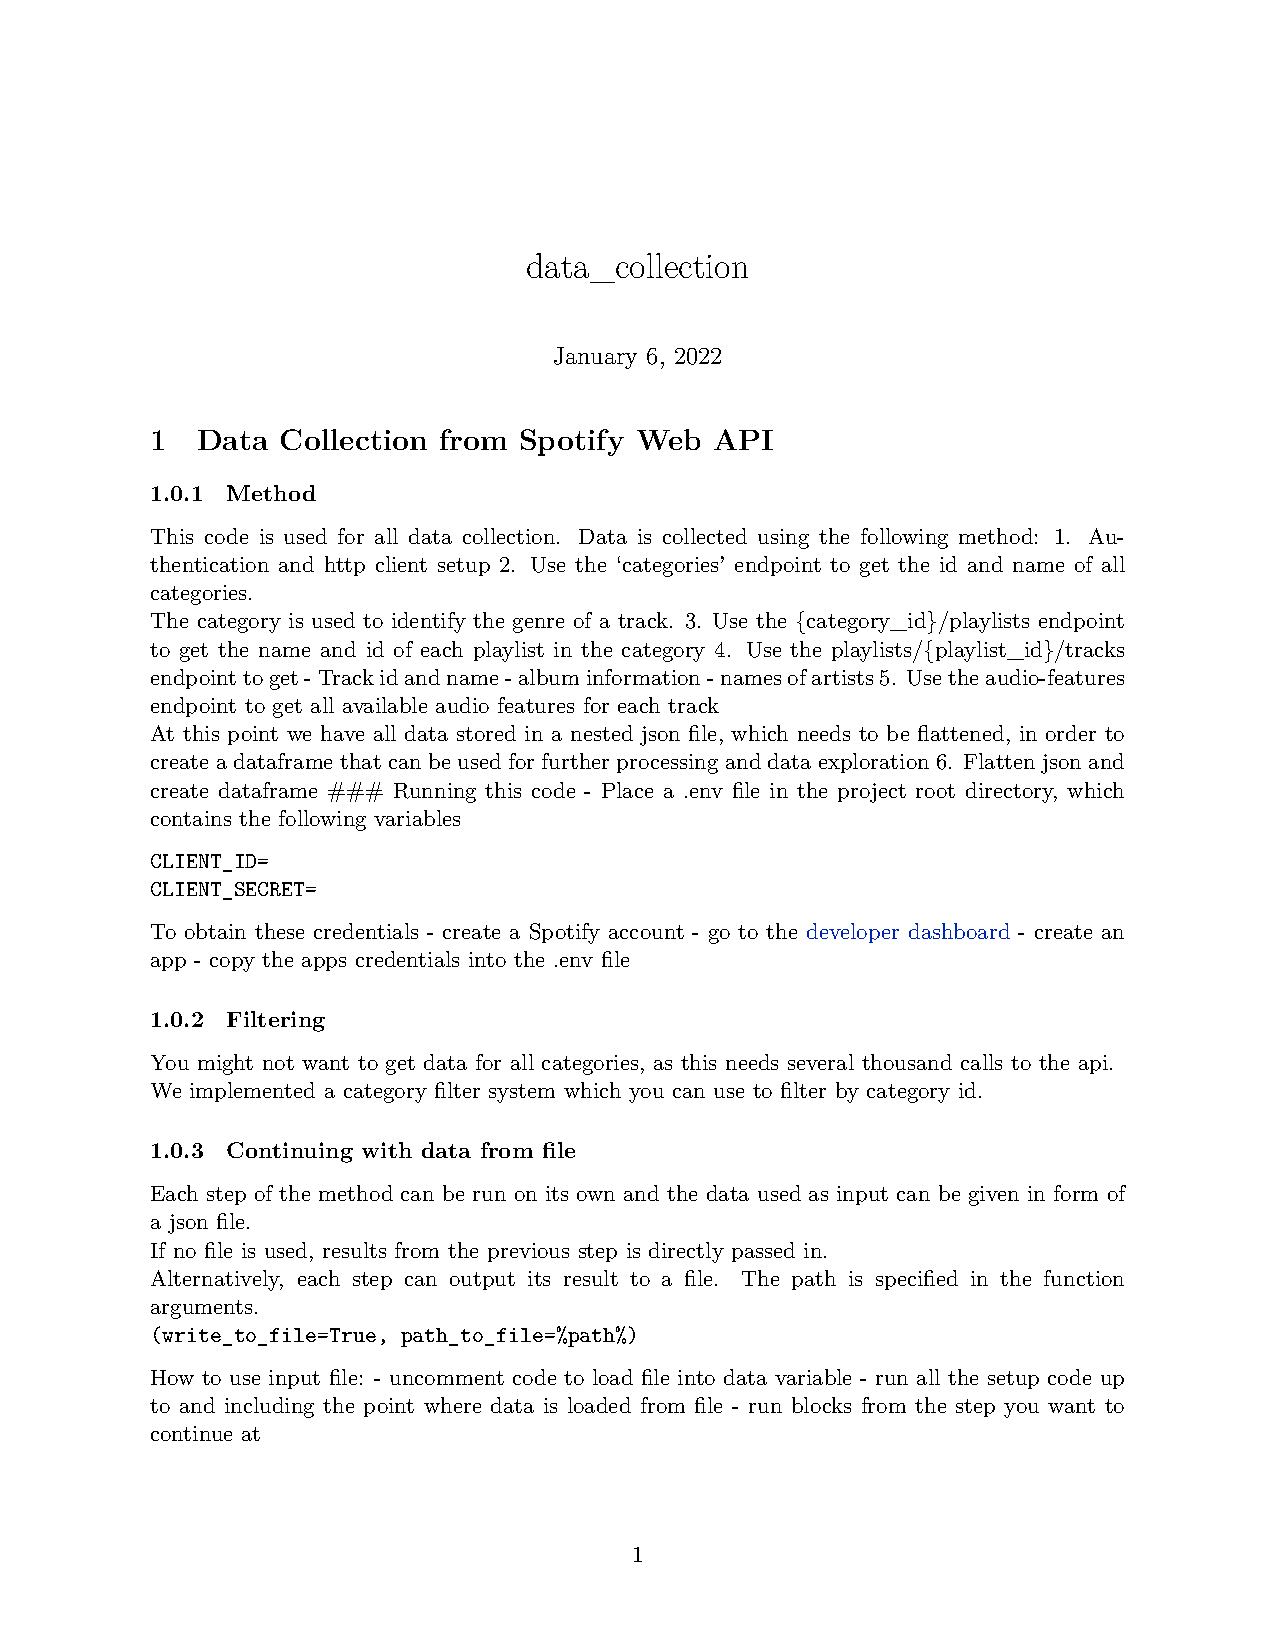
\includepdf[pages=-,frame=true,scale=0.85]{source_code/data_collection.pdf} %, offset=75 -75

\newpage
\section{Coding for CRISP DM Process}
\label{sec:appendix_crisp_dm}
This includes all code for the implementation of data understanding, preparation,
modeling and evaluation.

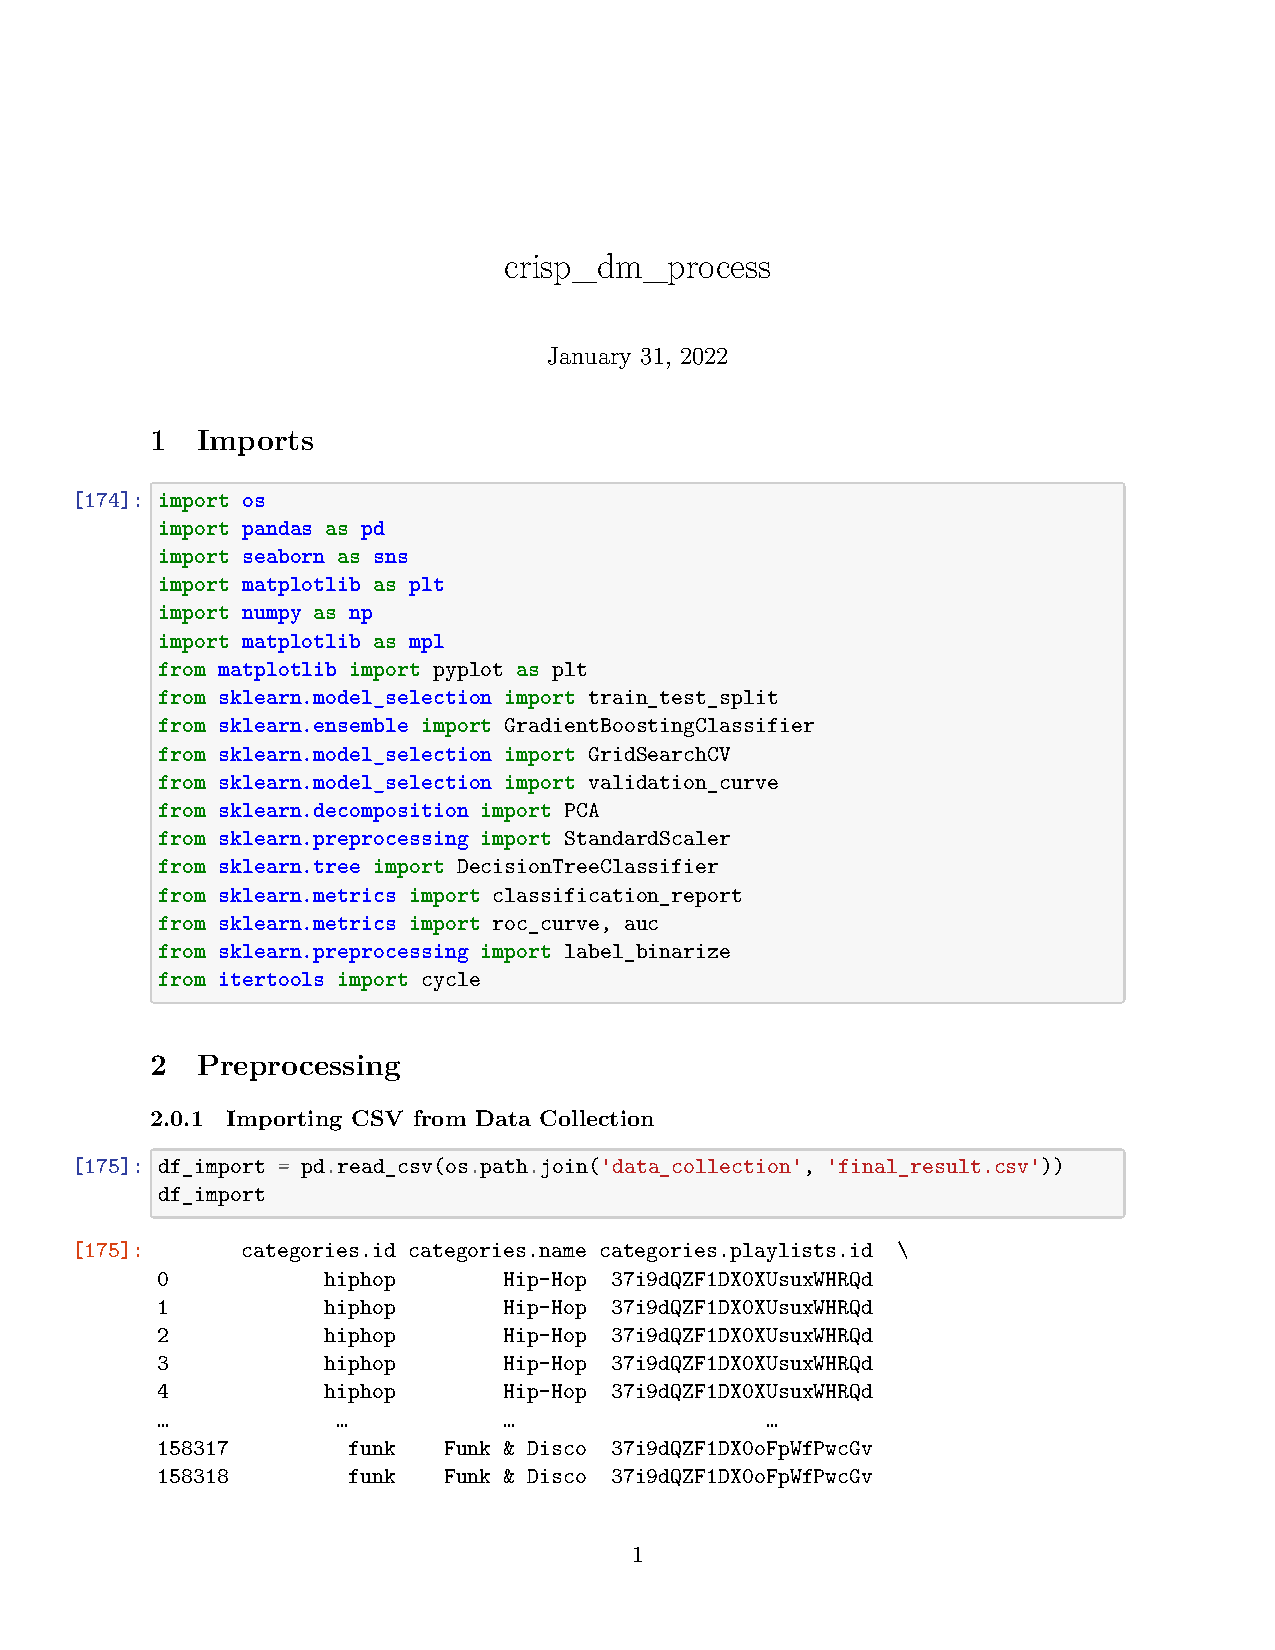
\includepdf[pages=-,frame=true,scale=0.85]{source_code/crisp_dm_process.pdf} %, offset=75 -75

\newpage
\section{Coding for Decision Tree Theory}
This is the code used to create the figures and tables for section \ref{sec:decision trees}
\label{sec:appendix_dt}

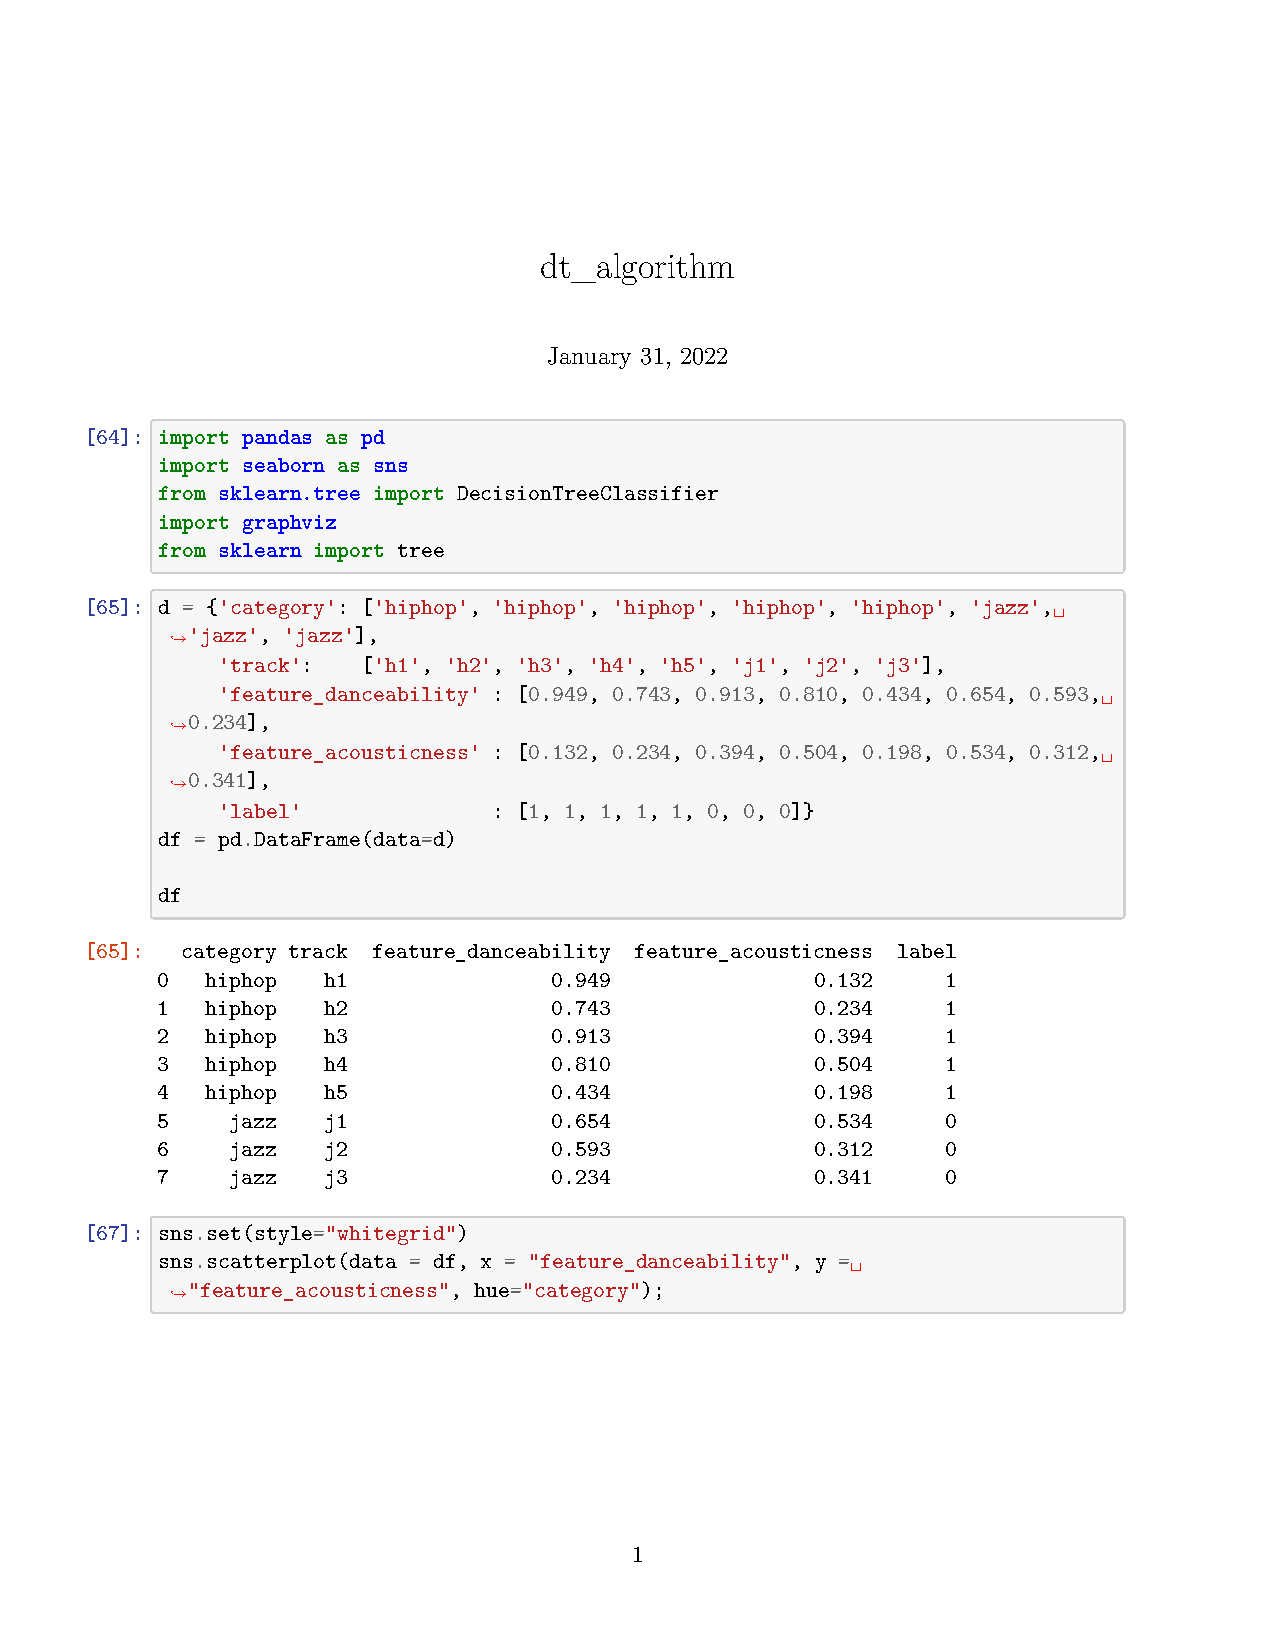
\includepdf[pages=-,frame=true,scale=0.85]{source_code/dt_algorithm.pdf} %, offset=75 -75

\newpage
\section{Coding for Gradient Boosting Theory}
This is the code used to create the figures and tables from section \ref{sec:Gradient Boosting}
\label{sec:appendix_gb}

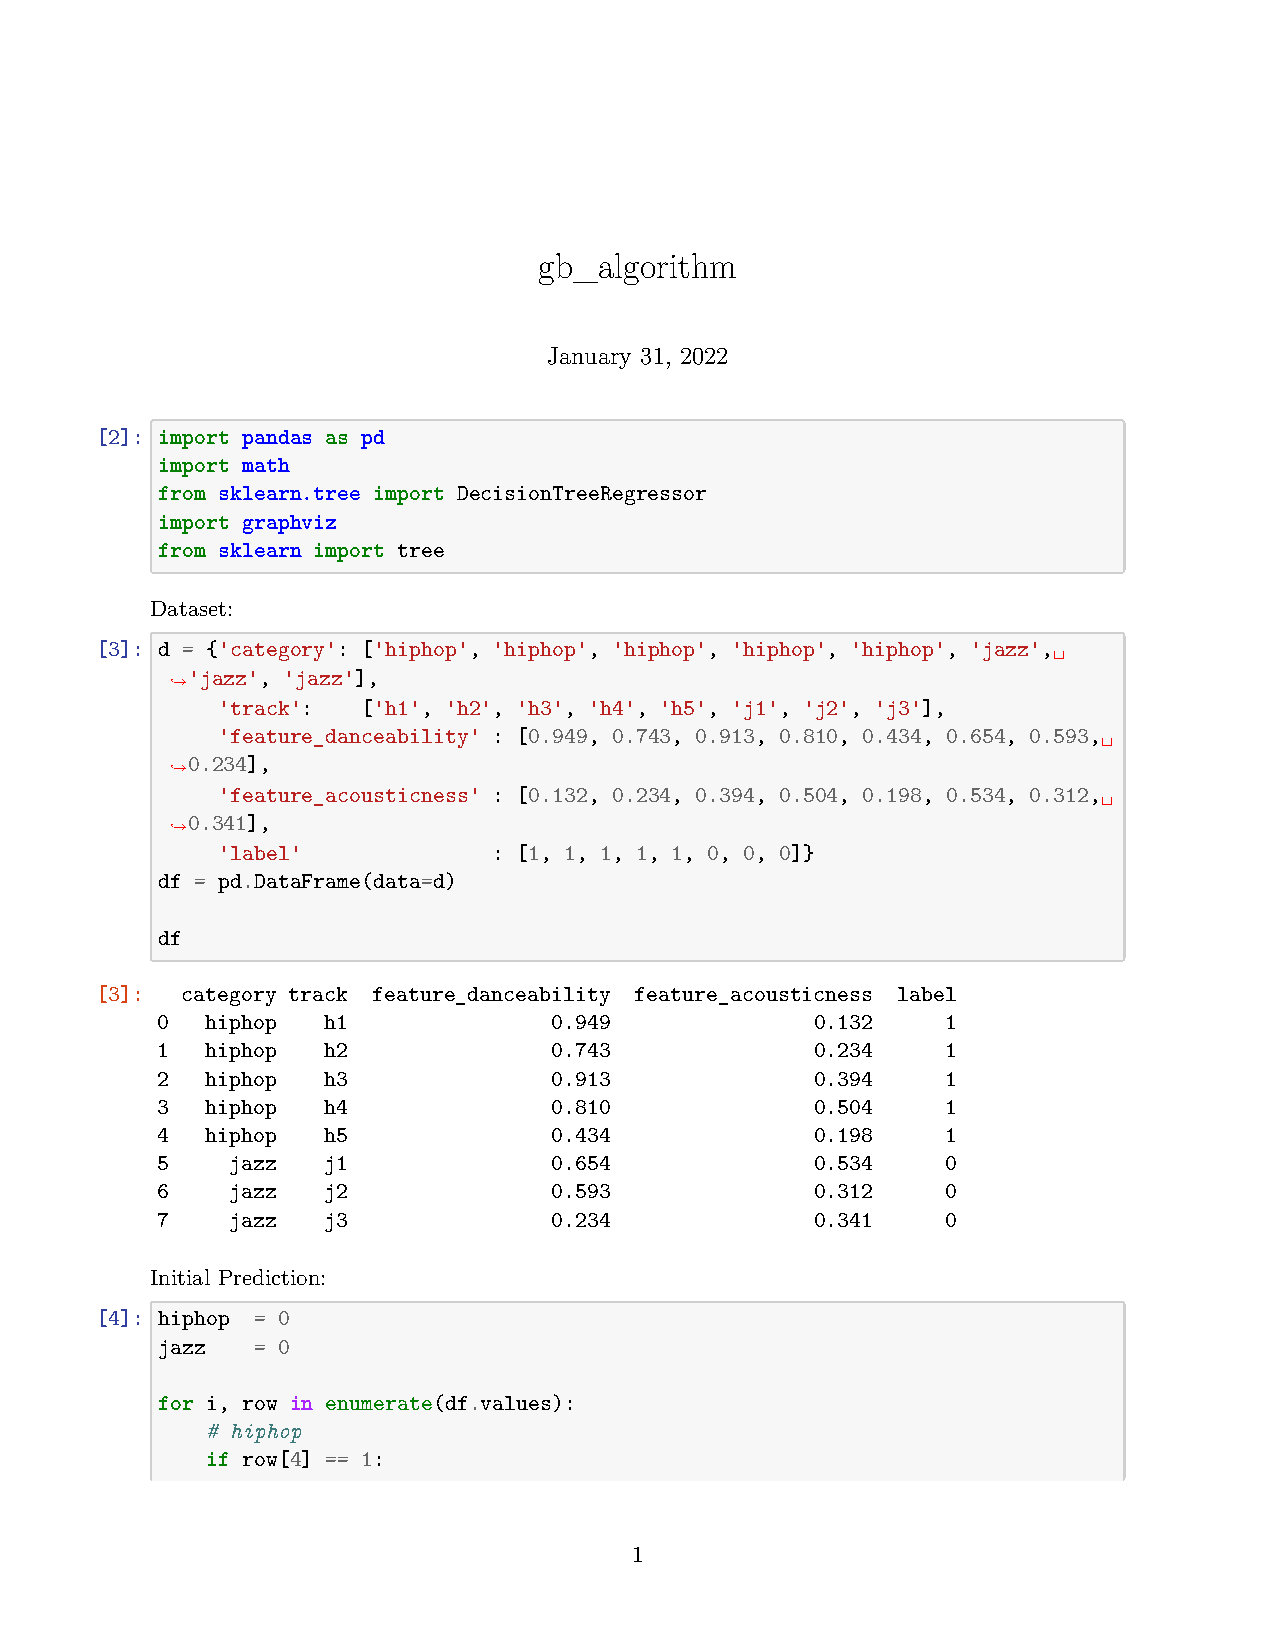
\includepdf[pages=-,frame=true,scale=0.85]{source_code/gb_algorithm.pdf} %, offset=75 -75
\end{appendices}
\addtocontents{toc}{\protect\setcounter{tocdepth}{2}}

%-----------------------------------
% Literaturverzeichnis
%-----------------------------------
\newpage

% Die folgende Zeile trägt ALLE Werke aus literatur.bib in das
% Literaturverzeichnis ein, egal ob sie zietiert wurden oder nicht.
% Der Befehl ist also nur zum Test der Skripte sinnvoll und muss bei echten
% Arbeiten entfernt werden.
%\nocite{*}

%\addcontentsline{toc}{section}{Literatur}

% Die folgenden beiden Befehle würden ab dem Literaturverzeichnis wieder eine
% römische Seitennummerierung nutzen.
% Das ist nach dem Leitfaden nicht zu tun. Dort steht nur dass 'sämtliche
% Verzeichnisse VOR dem Textteil' römisch zu nummerieren sind. (vgl. S. 3)
%\pagenumbering{Roman} %Zähler wieder römisch ausgeben
%\setcounter{page}{4}  %Zähler manuell hochsetzen

% Ausgabe des Literaturverzeichnisses

% Keine Trennung der Werke im Literaturverzeichnis nach ihrer Art
% (Online/nicht-Online)
%\begin{RaggedRight}
%\printbibliography
%\end{RaggedRight}

% Alternative Darstellung, die laut Leitfaden genutzt werden sollte.
% Dazu die Zeilen auskommentieren und folgenden code verwenden:

% Literaturverzeichnis getrennt nach Nicht-Online-Werken und Online-Werken
% (Internetquellen).
% Die Option nottype=online nimmt alles, was kein Online-Werk ist.
% Die Option heading=bibintoc sorgt dafür, dass das Literaturverzeichnis im
% Inhaltsverzeichnis steht.
% Es ist übrigens auch möglich mehrere type- bzw. nottype-Optionen anzugeben, um
% noch weitere Arten von Zusammenfassungen eines Literaturverzeichnisse zu
% erzeugen.
% Beispiel: [type=book,type=article]
\printbibliography[nottype=online,heading=bibintoc,title={\langde{Literaturverzeichnis}\langen{Bibliography}}]

% neue Seite für Internetquellen-Verzeichnis
\newpage

% Laut Leitfaden 2018, S. 14, Fussnote 44 stehen die Internetquellen NICHT im
% Inhaltsverzeichnis, sondern gehören zum Literaturverzeichnis.
% Die Option heading=bibintoc würde die Internetquelle als eigenen Eintrag im
% Inhaltsverzeicnis anzeigen.
%\printbibliography[type=online,heading=bibintoc,title={\headingNameInternetSources}]
\printbibliography[type=online,heading=subbibliography,title={\headingNameInternetSources}]

\newpage
\pagenumbering{gobble} % Keine Seitenzahlen mehr

%-----------------------------------
% Ehrenwörtliche Erklärung
%-----------------------------------
\section*{%
	\langde{Ehrenwörtliche Erklärung}
	\langen{Declaration in lieu of oath}}
\langde{Hiermit versichere ich, dass die vorliegende Arbeit von mir selbstständig und ohne unerlaubte Hilfe angefertigt worden ist, insbesondere dass ich alle Stellen, die wörtlich oder annähernd wörtlich aus Veröffentlichungen entnommen sind, durch Zitate als solche gekennzeichnet habe. Ich versichere auch, dass die von mir eingereichte schriftliche Version mit der digitalen Version übereinstimmt. Weiterhin erkläre ich, dass die Arbeit in gleicher oder ähnlicher Form noch keiner Prüfungsbehörde/Prüfungsstelle vorgelegen hat. Ich erkläre mich damit einverstanden, dass die Arbeit der Öffentlichkeit zugänglich gemacht wird. Ich erkläre mich damit einverstanden, dass die Digitalversion dieser Arbeit zwecks Plagiatsprüfung auf die Server externer Anbieter hochgeladen werden darf. Die Plagiatsprüfung stellt keine Zurverfügungstellung für die Öffentlichkeit dar.}
\langen{I hereby declare that I produced the submitted paper with no assistance from any other party and without the use of any unauthorized aids and, in particular, that I have marked as quotations all passages which are reproduced verbatim or near-verbatim from publications. Also, I declare that the submitted print version of this thesis is identical with its digital version. Further, I declare that this thesis has never been submitted before to any examination board in either its present form or in any other similar version. I herewith agree that this thesis may be published. I herewith consent that this thesis may be uploaded to the server of external contractors for the purpose of submitting it to the contractors’ plagiarism detection systems. Uploading this thesis for the purpose of submitting it to plagiarism detection systems is not a form of publication.}


\par\medskip
\par\medskip

\vspace{5cm}

\begin{table}[H]
	\centering
	\begin{tabular*}{\textwidth}{c @{\extracolsep{\fill}} ccccc}
		& Thomas Keiser \\
		& Martin Krüger \\
		& Luis Pflamminger \\
		\myOrt, \the\day.\the\month.\the\year
		&
		Jesper Wesemann \\
		% Hinterlege deine eingescannte Unterschrift im Verzeichnis /abbildungen und nenne sie unterschrift.png
		% Bilder mit transparentem Hintergrund können teils zu Problemen führen
		%
\includegraphics[width=0.35\textwidth]{unterschrift}\vspace*{-0.35cm}
		\rule[0.5ex]{12em}{0.55pt} & \rule[0.5ex]{12em}{0.55pt} \\
		\langde{(Ort, Datum)}\langen{(Location, Date)} & \langde{(Eigenhändige Unterschrift)}\langen{(handwritten signature)}
		\\
	\end{tabular*} \\
\end{table}

\end{document}
